\section{Functions for Rough Interpolation}

We will focus on interpolation where the function is not continuous
or whose derivatives are not continuous and compare the results
with standard Chebyshev interpolation and Chebyshev filters in 1D.
Because there are fewer theoretical results, we will focus on analyzing
some carefully chosen examples; in particular, we will
investigate interpolating
%
\begin{align}
    H(x) &= \begin{cases} 0 &x<0 \\ 1 &x\ge0 \end{cases} \nonumber\\
    H_{2}(x) &= H(x+\tfrac{1}{2}) + H(x) + H(x-\tfrac{1}{2}) \nonumber\\
    R(x) &= \begin{cases} \frac{1}{1+25x^{2}} &x<0 \\
                          \frac{2}{1+25x^{2}} &x\ge0 \end{cases} \nonumber\\
    G(x,\alpha) &= \abs{x}^{\alpha} \nonumber\\
    G_{2}(x,\alpha) &= G(x+\tfrac{1}{2},\alpha) + G(x,\alpha) +
        G(x-\tfrac{1}{2},\alpha).
\end{align}
%
Naturally, $H$ is the Heaviside function, $R$ has a jump discontinuity
between two Runge functions, and $G(\cdot,\alpha)$
has infinite derivatives at the origin when
$\alpha\in\parens{0,1}$.
All of these functions have difficulties at $x=0$, making them
challenging interpolation problems.
The error will be determined by computing the relative error at 1000 points
in $[-1,-0.1)\cup(0.1,1]$.
In the case of $H_{2}$ and $G_{2}$, the functions have multiple difficulties
and the relative error will be computed in the region
$[-1,-0.6)\cup(-0.4,-0.1)\cup(0.1,0.4)\cup(0.6,1]$.

\section{Results for Fast MSN Interpolation in 1D for Rough Functions}
\label{sec:rough_1D_sim}

\subsection{Interpolation Comparison}

The relative error results for the Heaviside function $H$ can be found in
Fig.~\ref{fig:rough_comparison_heaviside},
the results for the Runge jump function $R(x)$ can be found in
Fig.~\ref{fig:rough_comparison_runge_jump}, and
the results for $G(\cdot,0.5)$ can be found in
Fig.~\ref{fig:rough_comparison_sharp_func}.
In the case of having multiple difficulties, 
the results for $H_{2}$ can be found in
Fig.~\ref{fig:rough_comparison_heaviside_2}, while
the results for $G_{2}(\cdot,0.5)$ can be found in
Fig.~\ref{fig:rough_comparison_sharp_func_2}.
We note that the Sharpened Cosine Filter $\sigma_{4}$ is denoted
by ``Cos8'' in the legend.
We will keep the unfiltered Chebyshev interpolant in both filter plots
for reference.

In every instance, MSN interpolation with $s=4$ appears to have the
quickest error decrease while also reaching machine precision first.
The best Chebyshev filters appear to to be the Sharpened Cosine filter (Cos8)
as well as the higher order Exponential filters (order 6 and 8).
The error profiles are approximately the same in every instance,
regardless of whether the function is discontinuous ($H$ and $R$),
has infinite derivatives ($G$), or multiple jumps or infinite derivatives
($H_{2}$ and $G_{2}$).
The worst case for MSN interpolation is when $s=1$.
Even in this case, it has lower error than the Chebyshev,
Fej\'{e}r, Lanczos, Cosine, and Exp 2 filters in most instances.
To make the comparison clear, in Fig.~\ref{fig:msn_filter_comp_heaviside_2}
where we plot the minimum error for both MSN interpolation
and Chebyshev filters for the $H_{2}$ function.
As we can see, the minimal MSN error usually approximately the same or better
than the best filters.
To see how different $s$ values in MSN affect interpolation
results, we include plots for various $s$ values and interpolation
points when approximating $H_{2}$ in Fig.~\ref{fig:msn_n_s_heaviside_2}.

In these examples so far we only used polynomials of degree $2n$
for $n$ interpolation points; we have included results for
degree $2n$, $4n$, $6n$, and $8n$ interpolation
in Fig.~\ref{fig:msn_comp_degree} when attempting to interpolate $H_{2}$.
As we can see, there is little difference between them.
The difference in using larger interpolation degree only becomes
apparent when using small $s$ values, such as when $s\in\parens{0,1}$.
By looking at the explicit form of the coefficients, we see
that they do not play a large part; furthermore, by construction,
once the IDCT gives somewhat accurate approximates of the true
Chebyshev coefficients, larger $s$ values closely match the
first $n$ coefficients while also matching the interpolation constraints.
Thus, degree $2n$ MSN interpolation appears sufficient in these tests.

% Print results for comparing MSN with Heaviside jump function

\begin{figure}[p]
    \centering
    \begin{subfigure}{0.45\textwidth}
    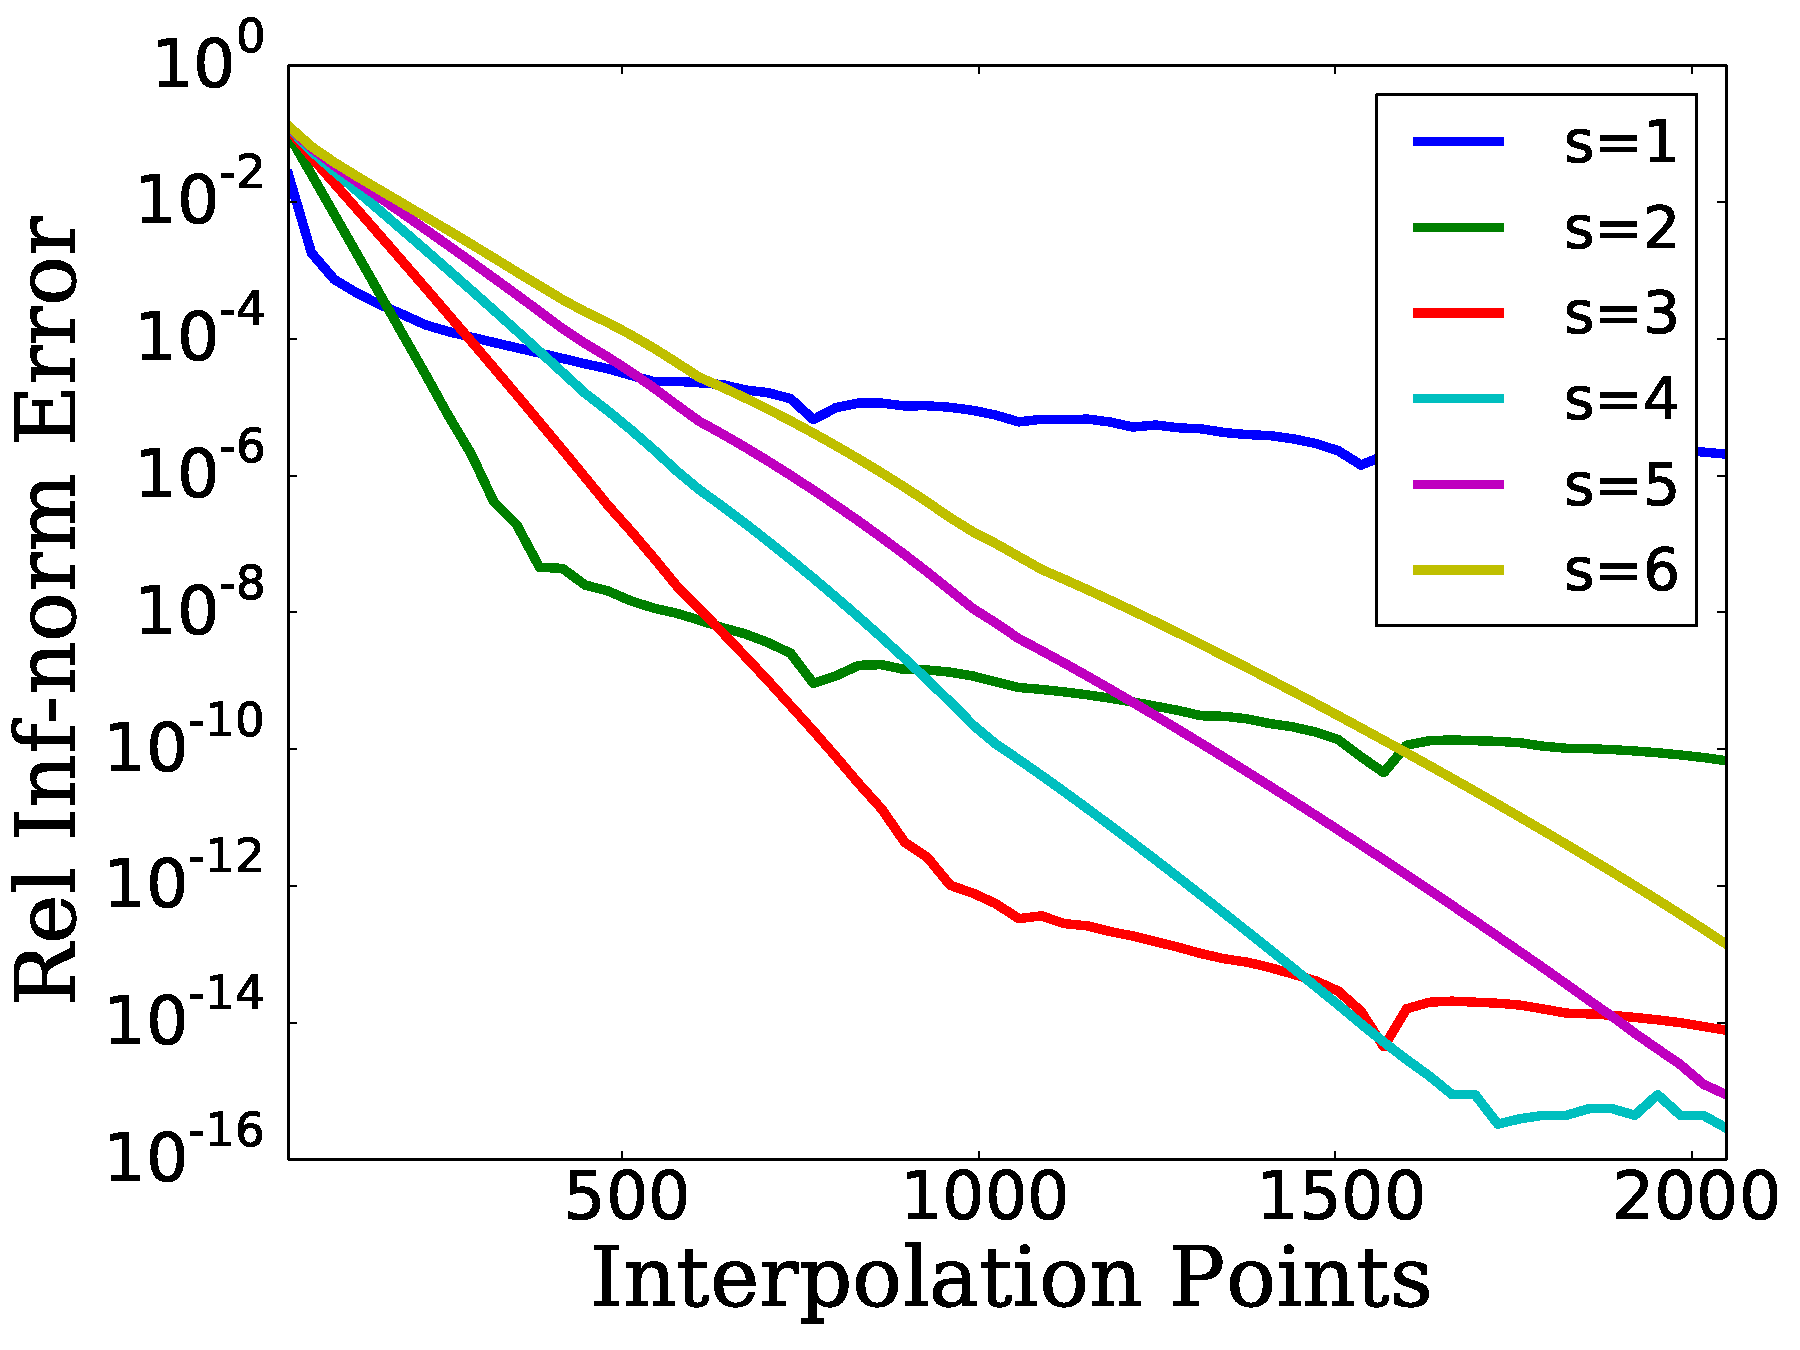
\includegraphics[width=\textwidth]{plots/msn_interp_fast_2n_rough_heaviside.pdf}
    \caption{MSN Interpolation}
    \end{subfigure}

    \begin{subfigure}{0.45\textwidth}
    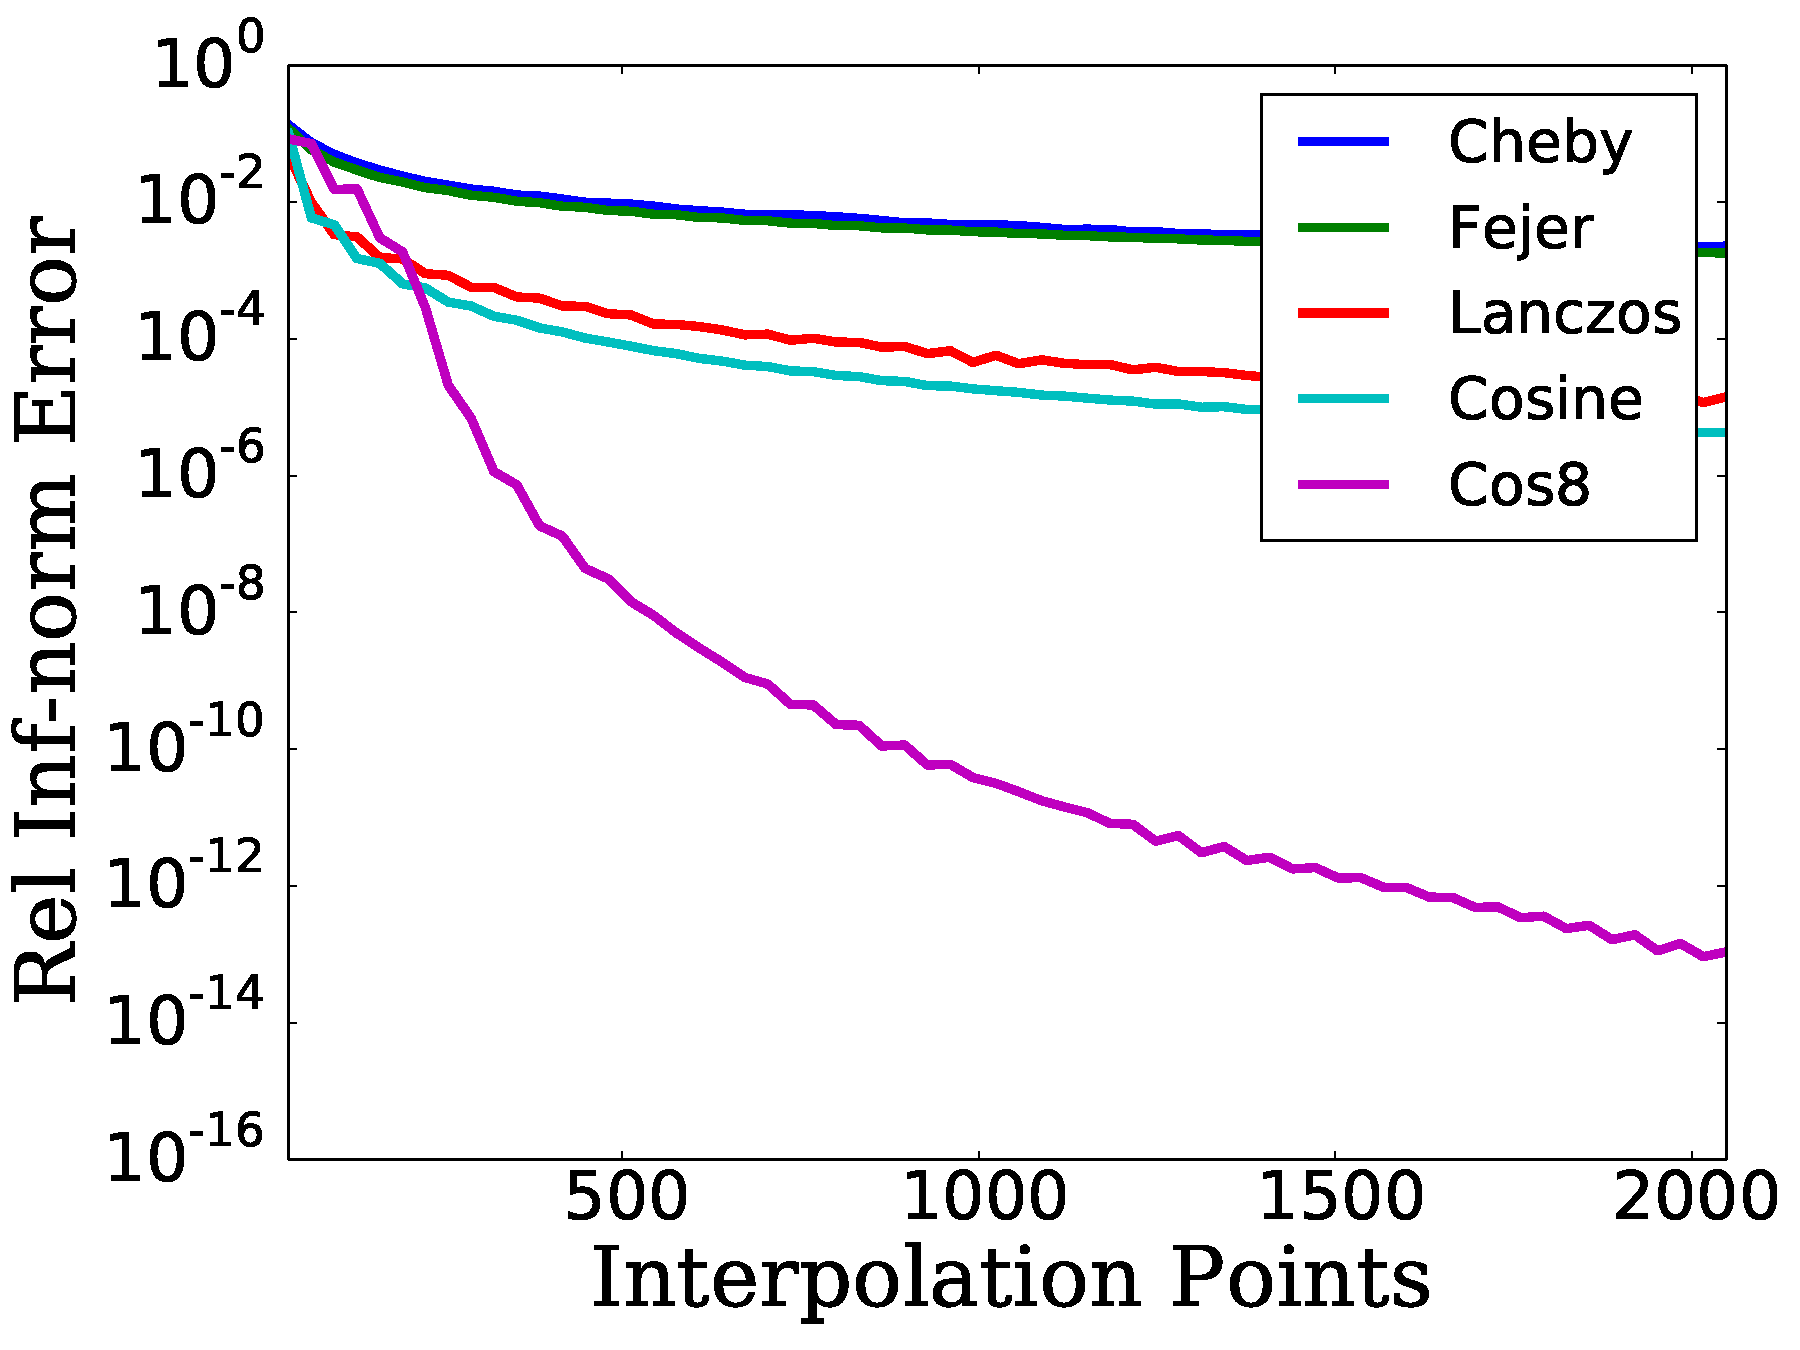
\includegraphics[width=\textwidth]{plots/cheby_interp_filter_rough_heaviside.pdf}
    \caption{Filters, Plot 1}
    \end{subfigure}
    \begin{subfigure}{0.45\textwidth}
    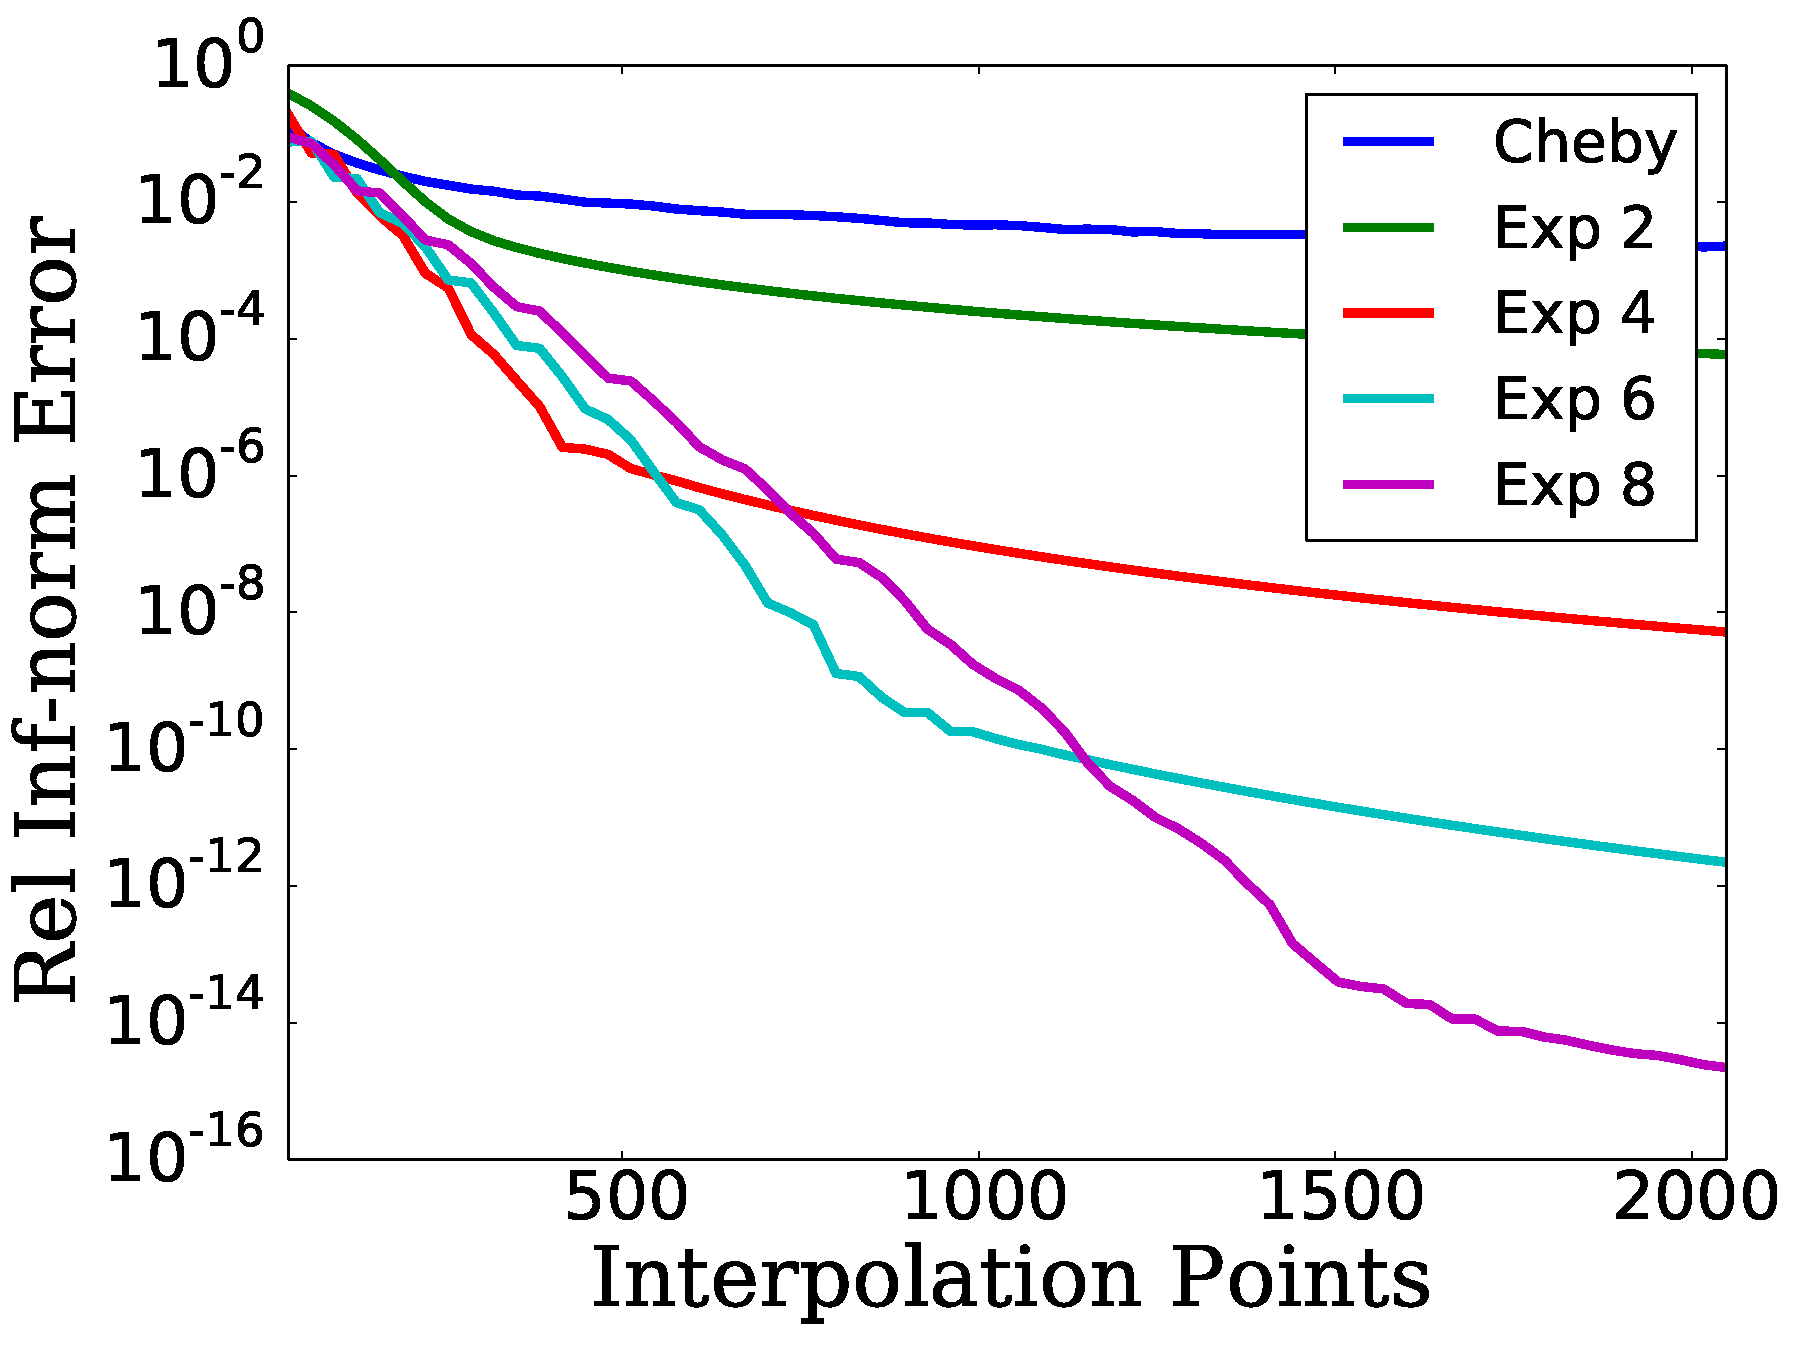
\includegraphics[width=\textwidth]{plots/cheby_interp_filter_2_rough_heaviside.pdf}
    \caption{Filters, Plot 2}
    \end{subfigure}
\caption[Rough Interpolation Comparison: Heaviside Jump Function]{
MSN interpolation and Chebyshev filtering results of the Heaviside jump
function $H$ for various $s$ values and filters.
We include standard Chebyshev interpolant in both filter examples for reference.
}
\label{fig:rough_comparison_heaviside}
\end{figure}




% Print results for comparing MSN with Heaviside jump function

\begin{figure}[p]
    \centering
    \begin{subfigure}{0.45\textwidth}
    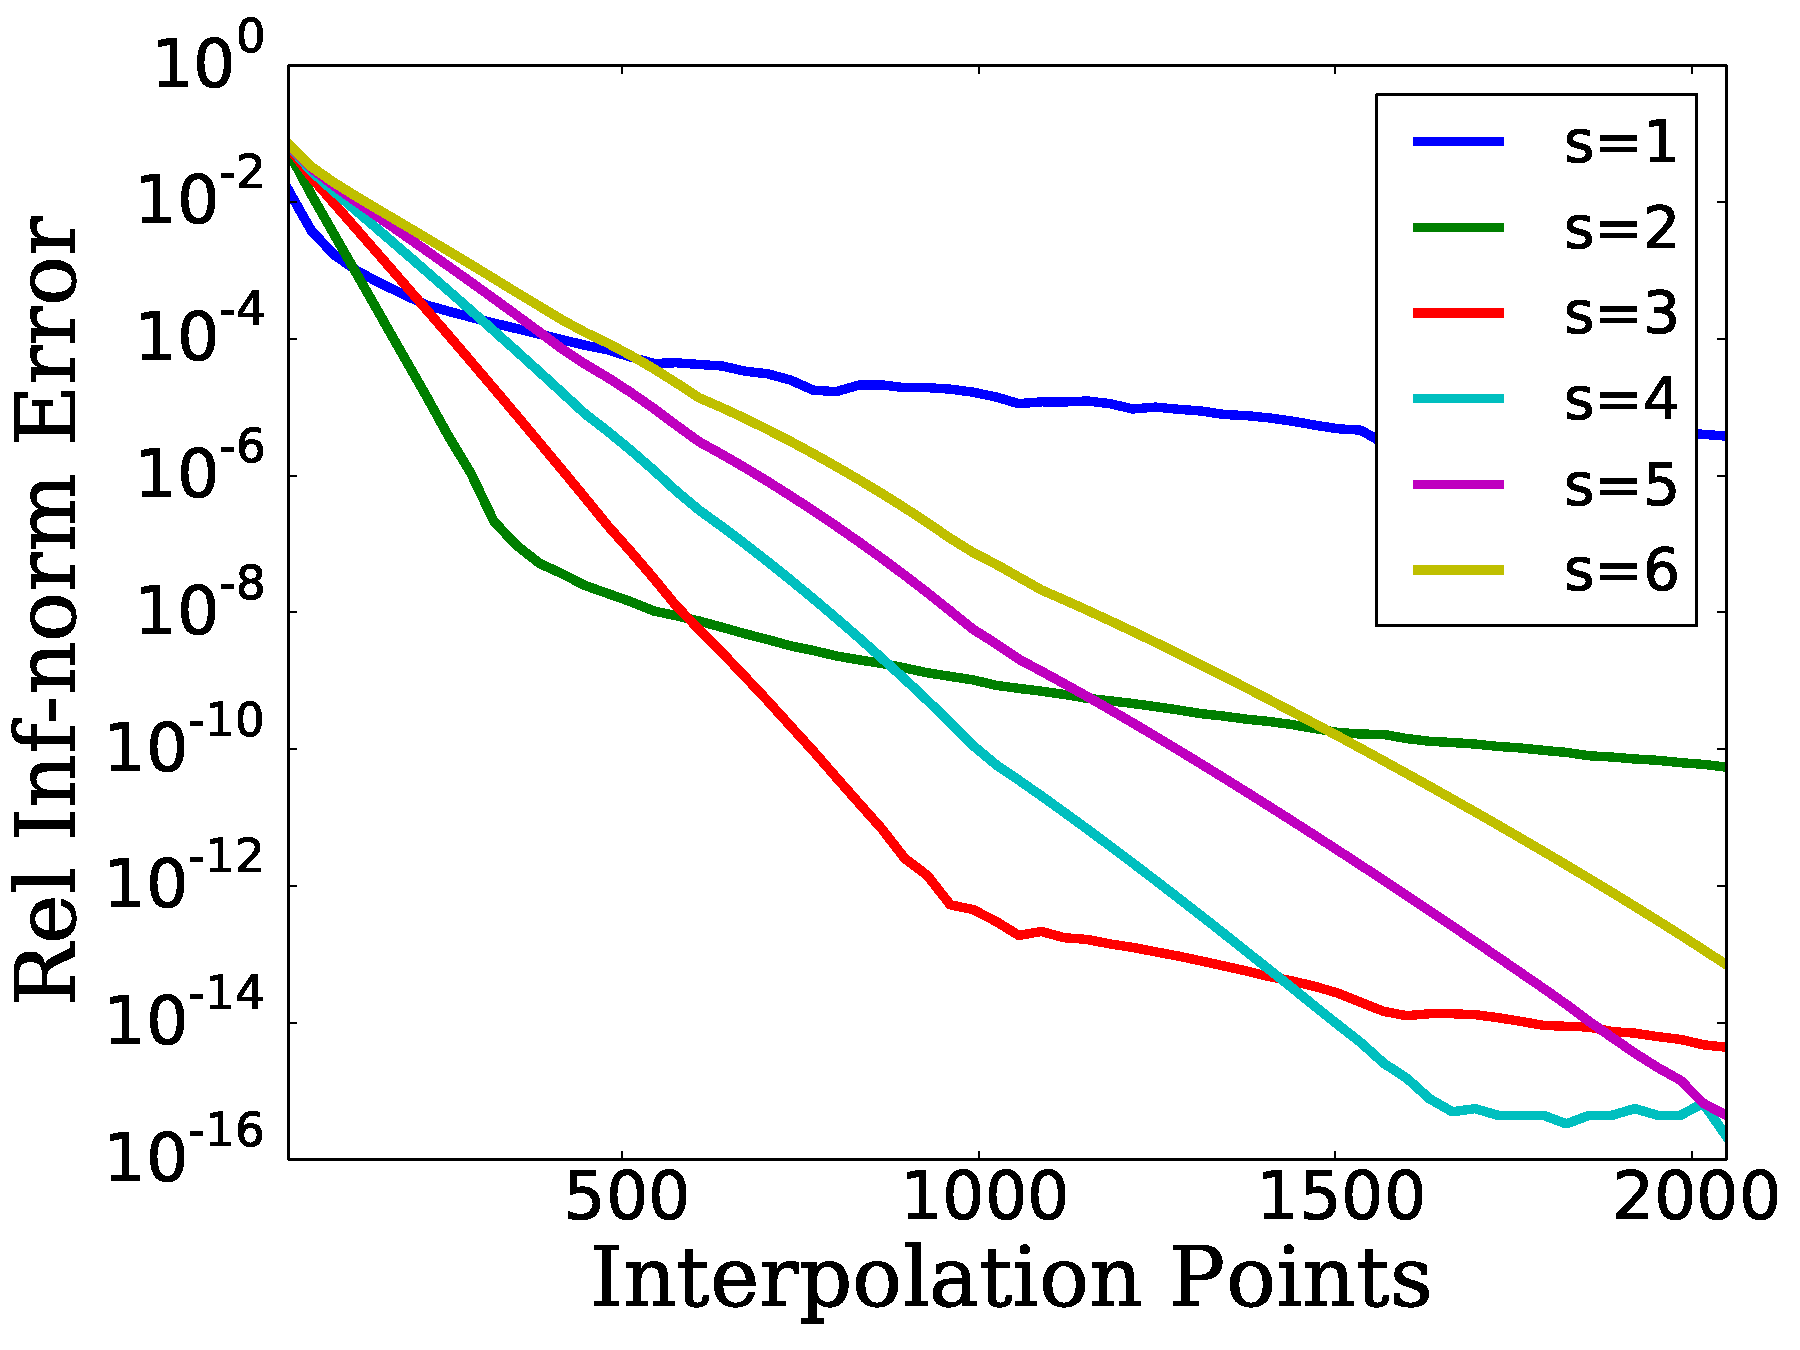
\includegraphics[width=\textwidth]{plots/msn_interp_fast_2n_rough_runge_jump.pdf}
    \caption{MSN Interpolation}
    \end{subfigure}

    \begin{subfigure}{0.45\textwidth}
    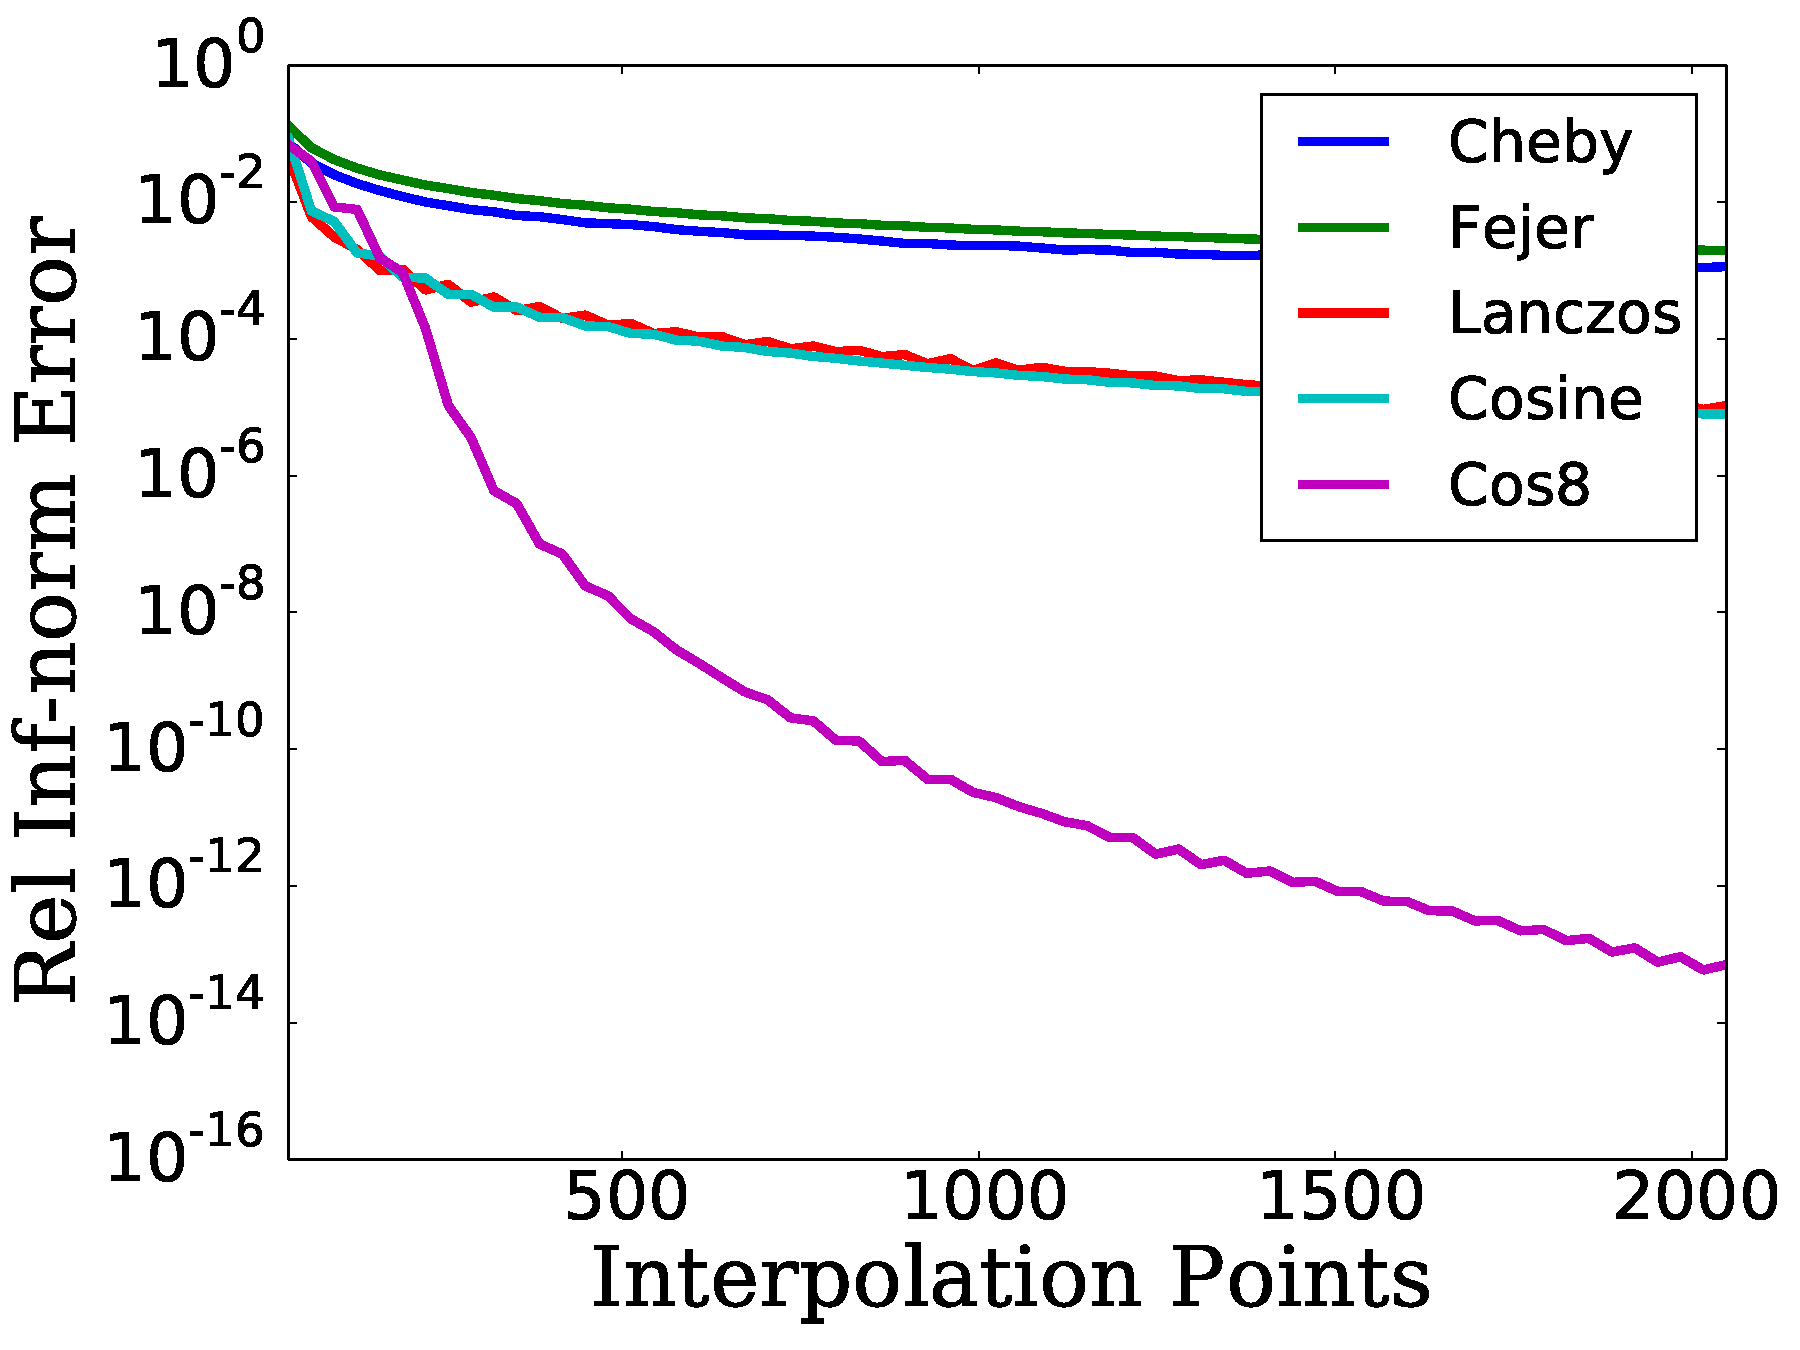
\includegraphics[width=\textwidth]{plots/cheby_interp_filter_rough_runge_jump.pdf}
    \caption{Filters, Plot 1}
    \end{subfigure}
    \begin{subfigure}{0.45\textwidth}
    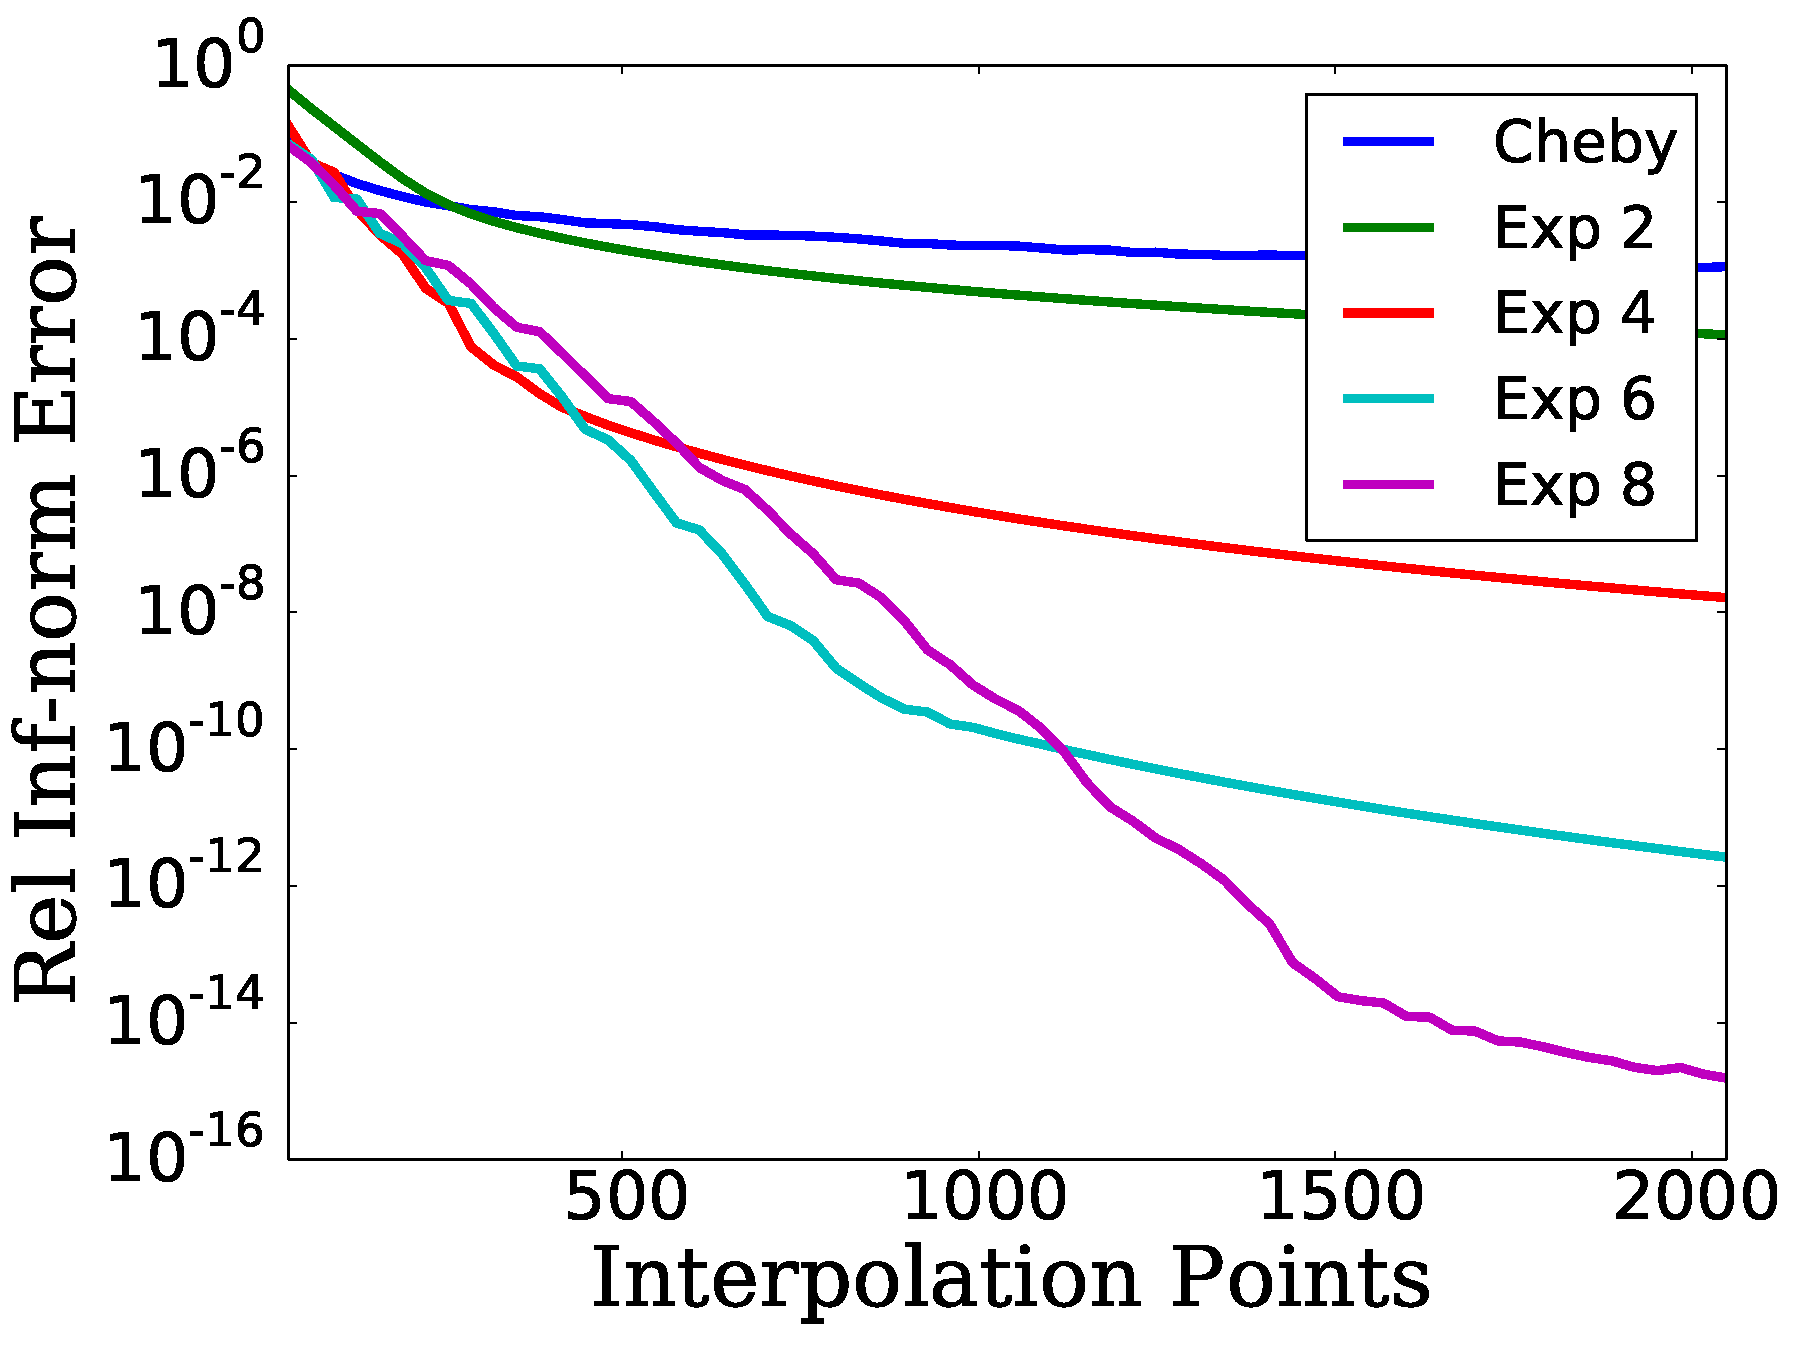
\includegraphics[width=\textwidth]{plots/cheby_interp_filter_2_rough_runge_jump.pdf}
    \caption{Filters, Plot 2}
    \end{subfigure}
\caption[Rough Interpolation Comparison: Runge Jump Function]{
MSN interpolation and Chebyshev filtering results of the Runge jump
function $R$ for various $s$ values and filters.
We include standard Chebyshev interpolant in both filter examples for reference.
}
\label{fig:rough_comparison_runge_jump}
\end{figure}




% Print results for comparing MSN with Heaviside jump function

\begin{figure}[p]
    \centering
    \begin{subfigure}{0.45\textwidth}
    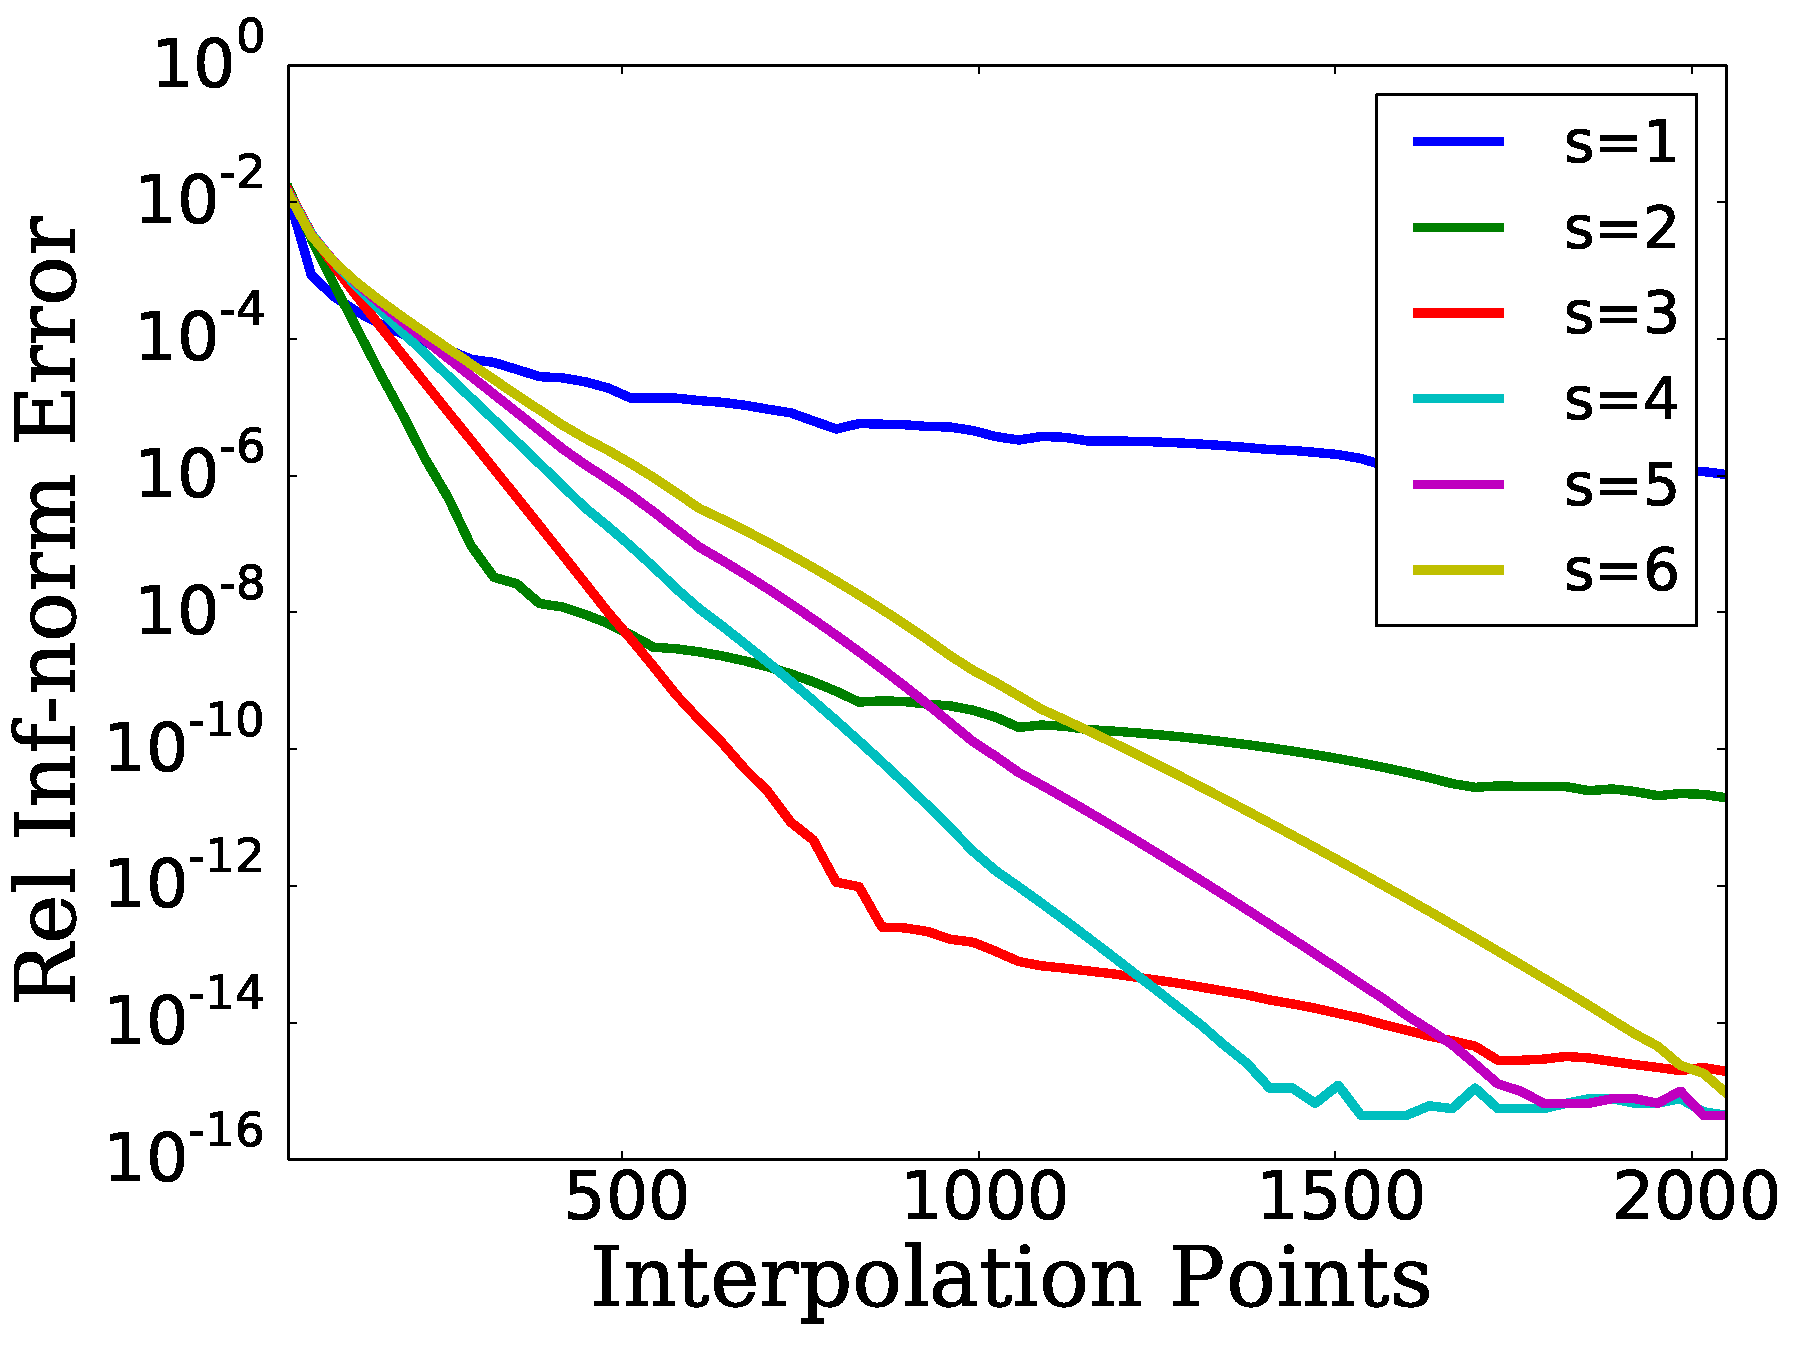
\includegraphics[width=\textwidth]{plots/msn_interp_fast_2n_rough_sharp_func.pdf}
    \caption{MSN Interpolation}
    \end{subfigure}

    \begin{subfigure}{0.45\textwidth}
    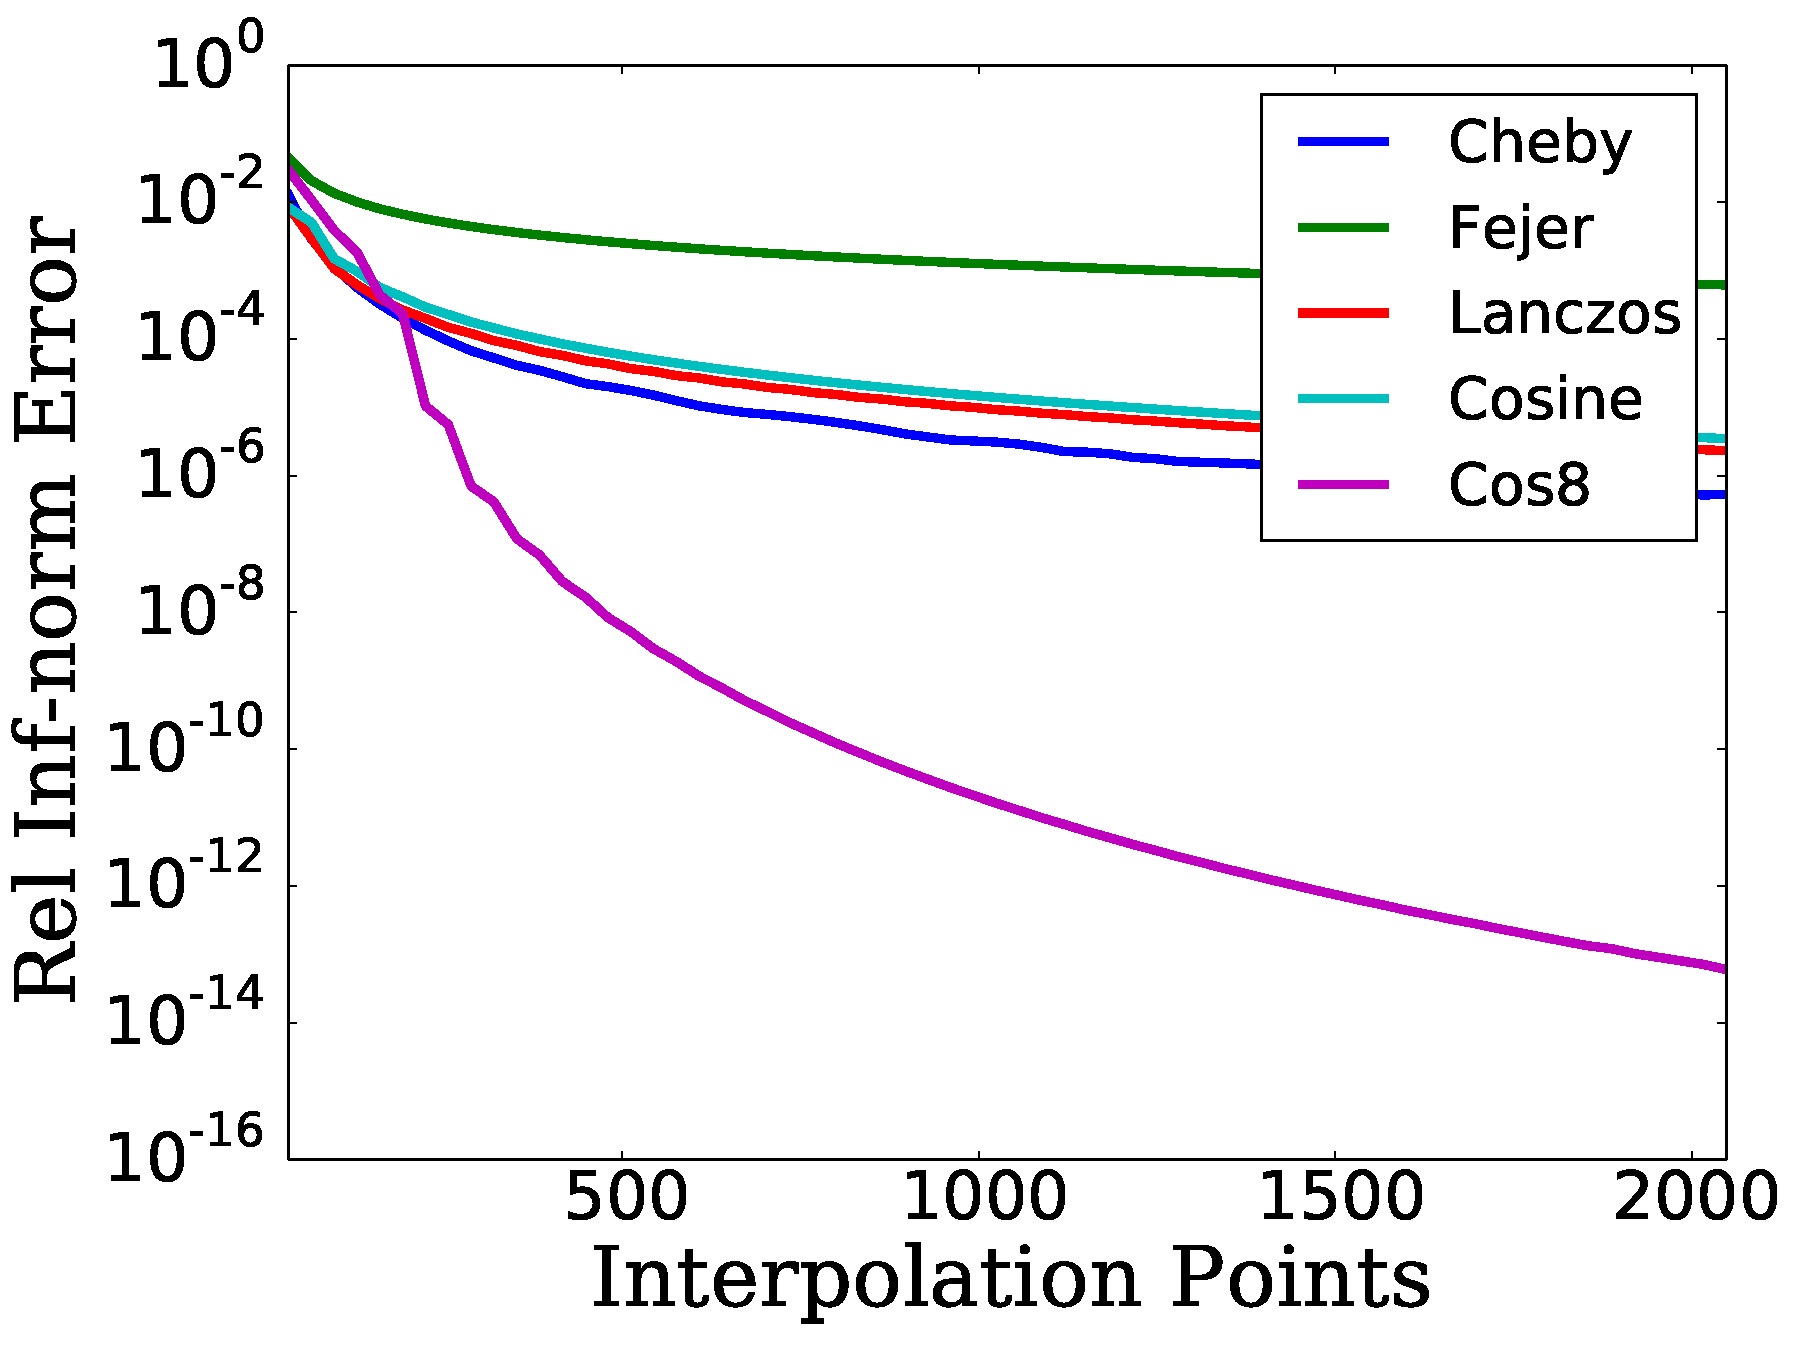
\includegraphics[width=\textwidth]{plots/cheby_interp_filter_rough_sharp_func.pdf}
    \caption{Filters, Plot 1}
    \end{subfigure}
    \begin{subfigure}{0.45\textwidth}
    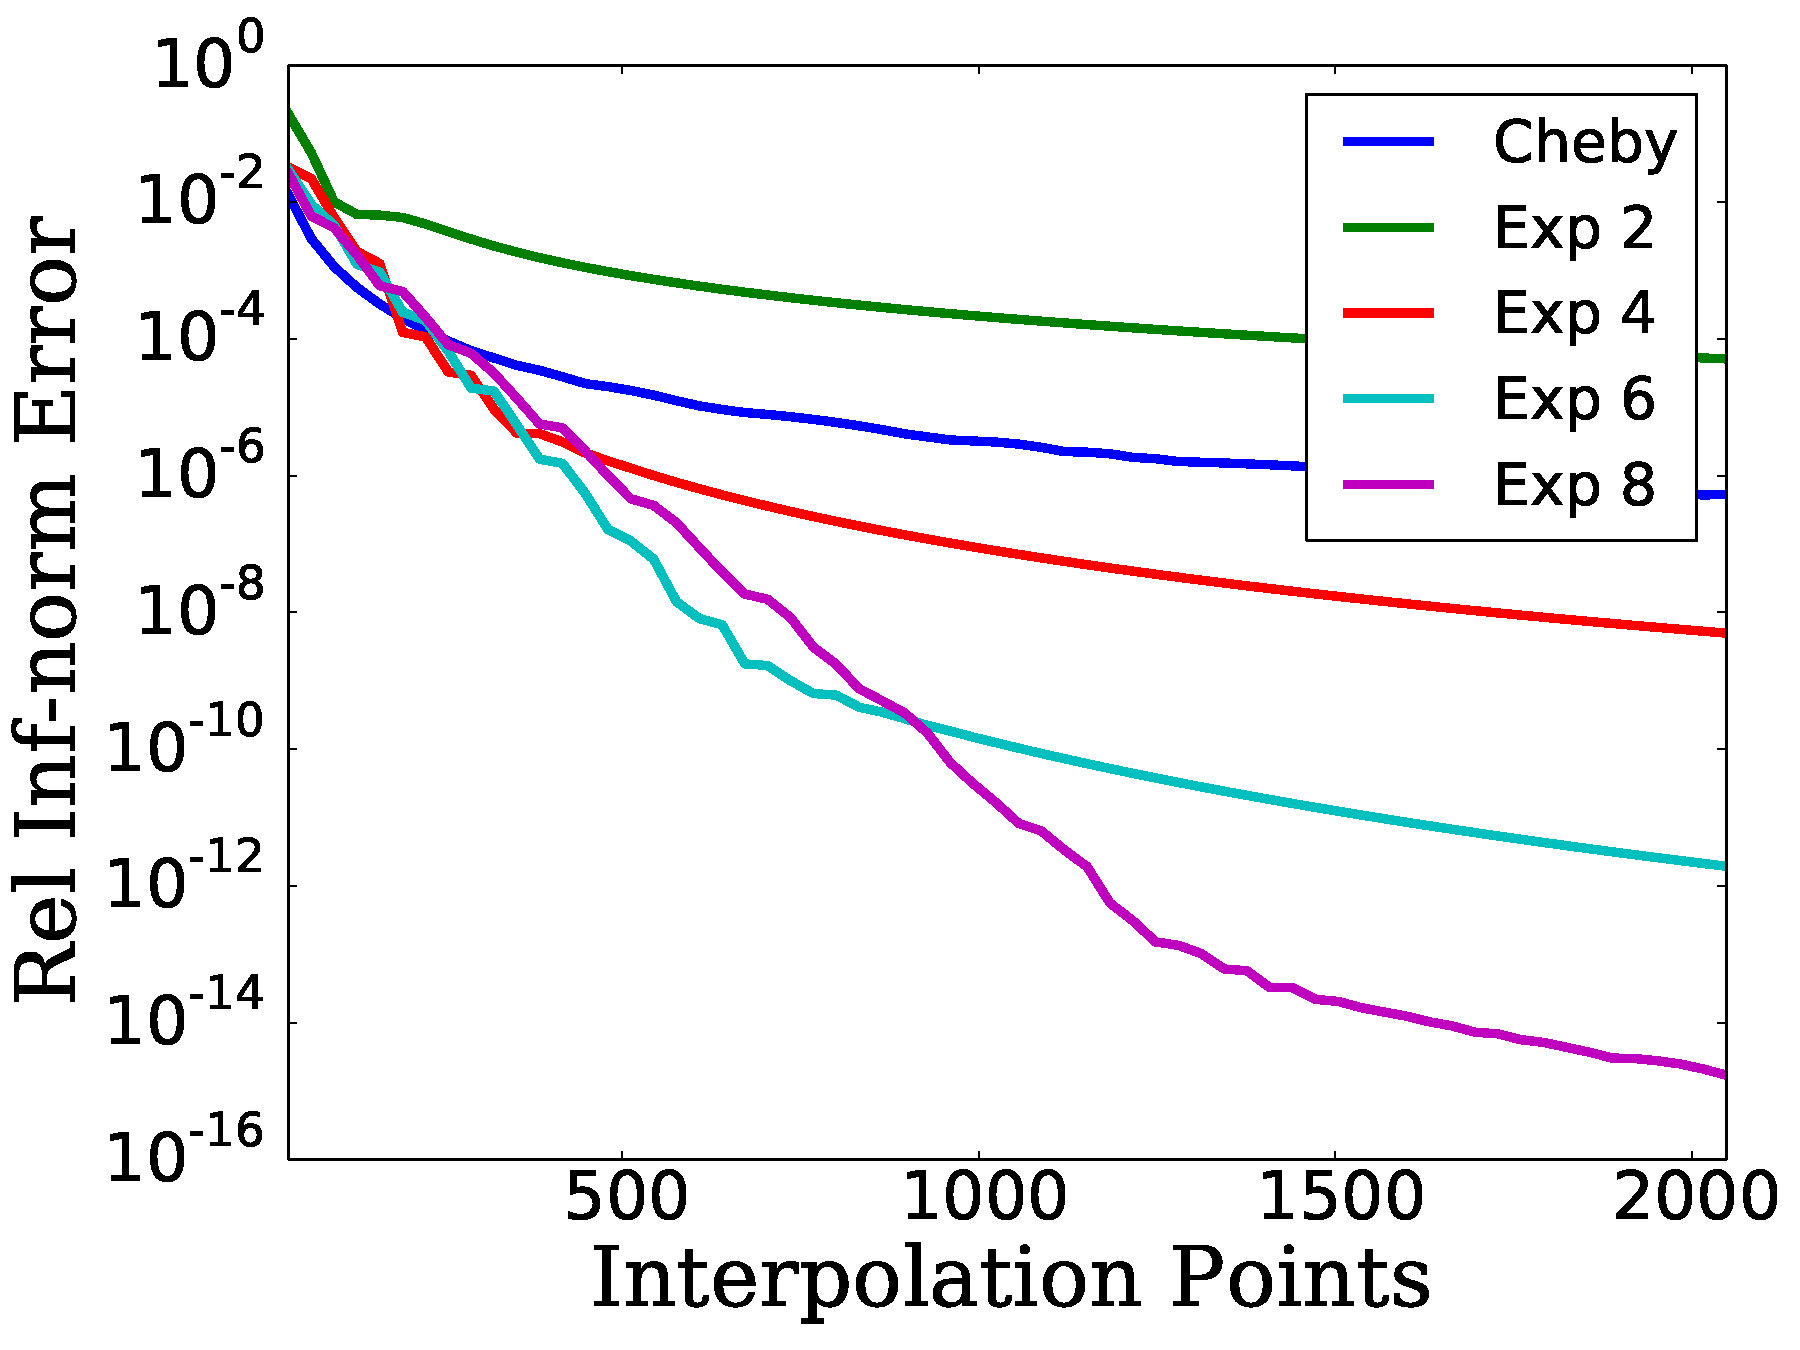
\includegraphics[width=\textwidth]{plots/cheby_interp_filter_2_rough_sharp_func.pdf}
    \caption{Filters, Plot 2}
    \end{subfigure}
\caption[Rough Interpolation Comparison: Sharp Function]{
MSN interpolation and Chebyshev filtering results of the Sharp Function
$G(\cdot,0.5)$ for various $s$ values and filters.
We include standard Chebyshev interpolant in both filter examples for reference.
}
\label{fig:rough_comparison_sharp_func}
\end{figure}




% Print results for comparing MSN with Heaviside jump function

\begin{figure}[p]
    \centering
    \begin{subfigure}{0.45\textwidth}
    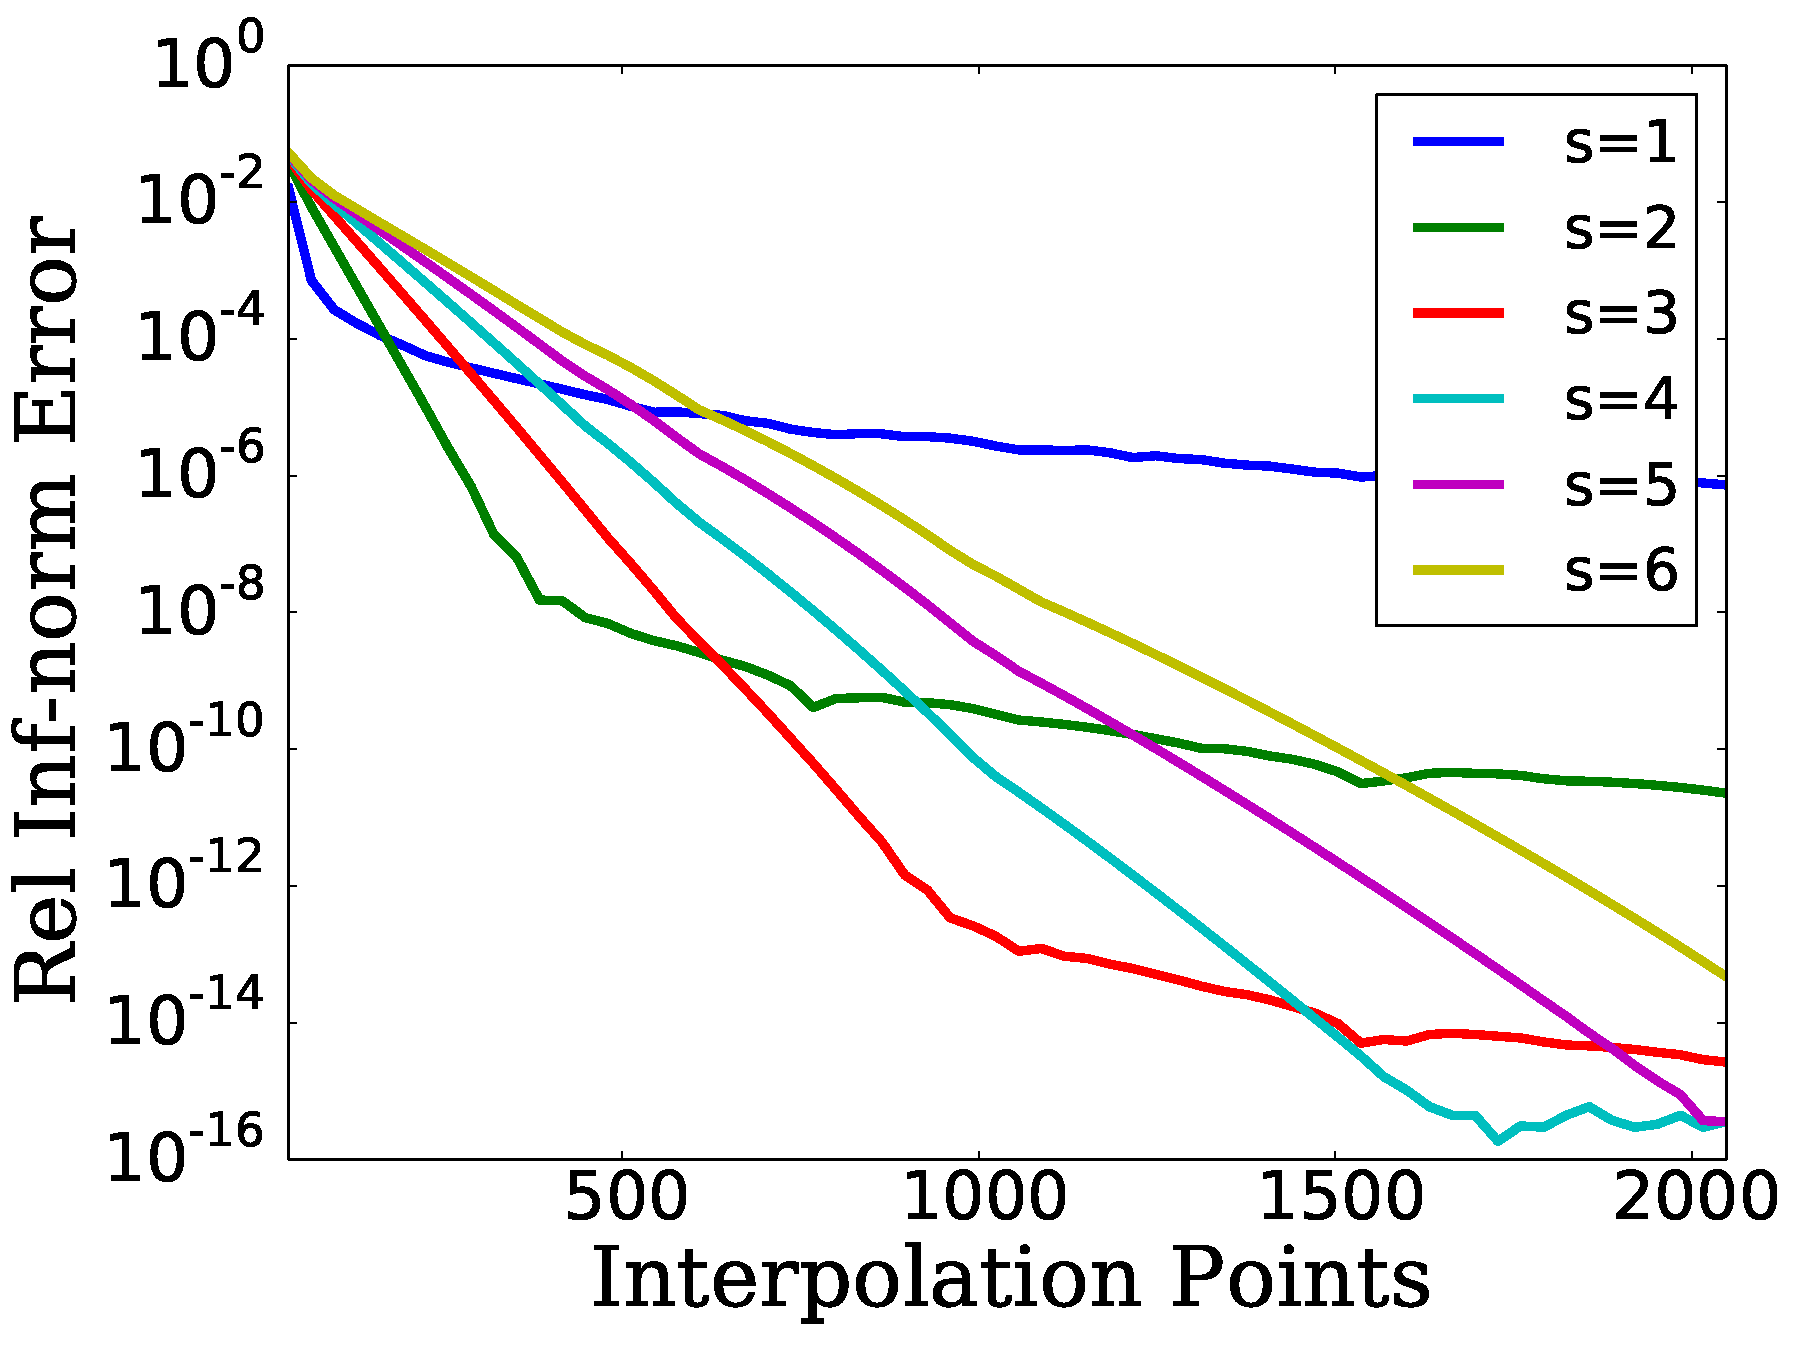
\includegraphics[width=\textwidth]{plots/msn_interp_fast_2n_rough_heaviside_2.pdf}
    \caption{MSN Interpolation}
    \end{subfigure}

    \begin{subfigure}{0.45\textwidth}
    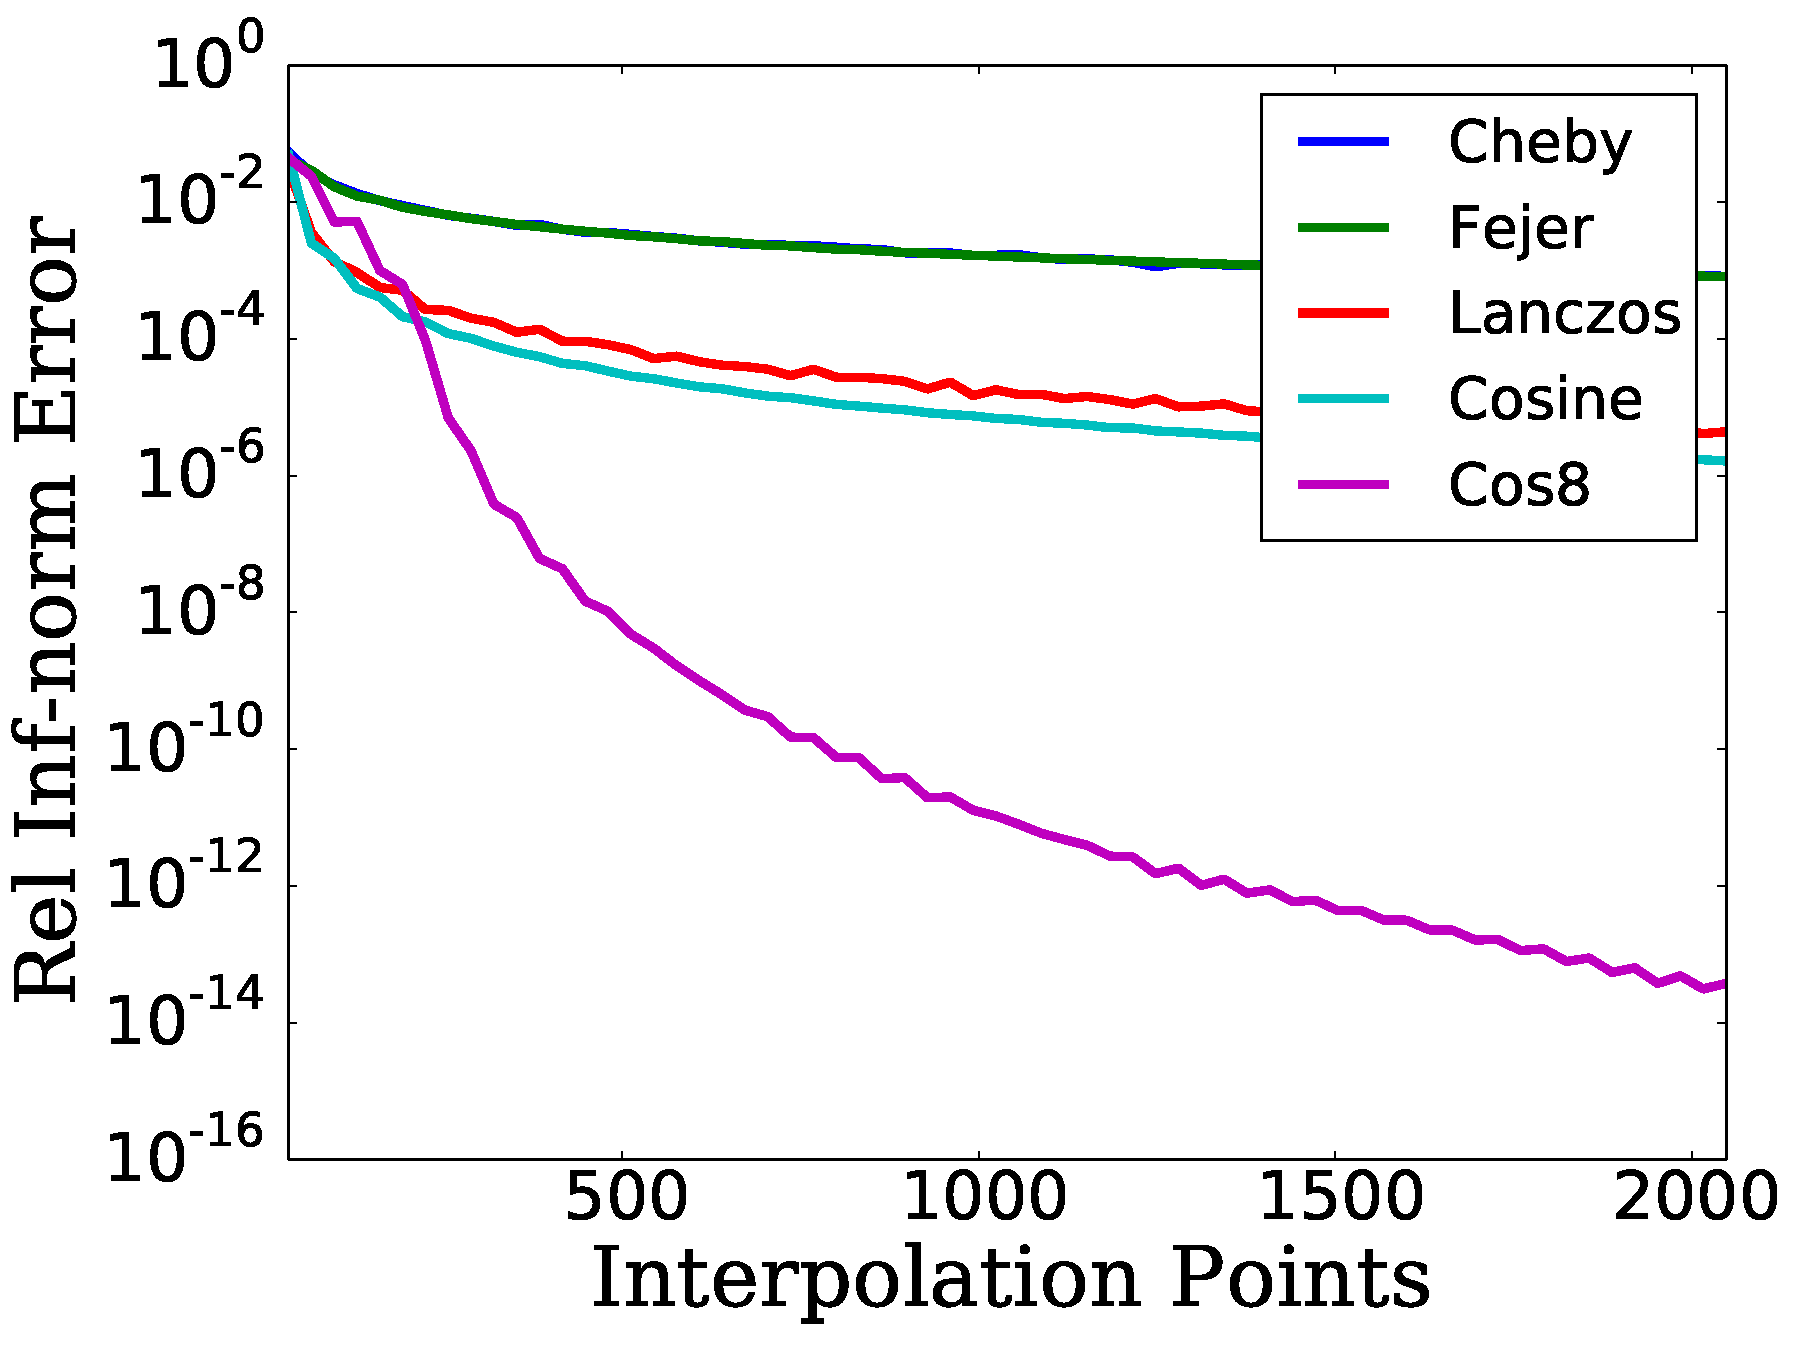
\includegraphics[width=\textwidth]{plots/cheby_interp_filter_rough_heaviside_2.pdf}
    \caption{Filters, Plot 1}
    \end{subfigure}
    \begin{subfigure}{0.45\textwidth}
    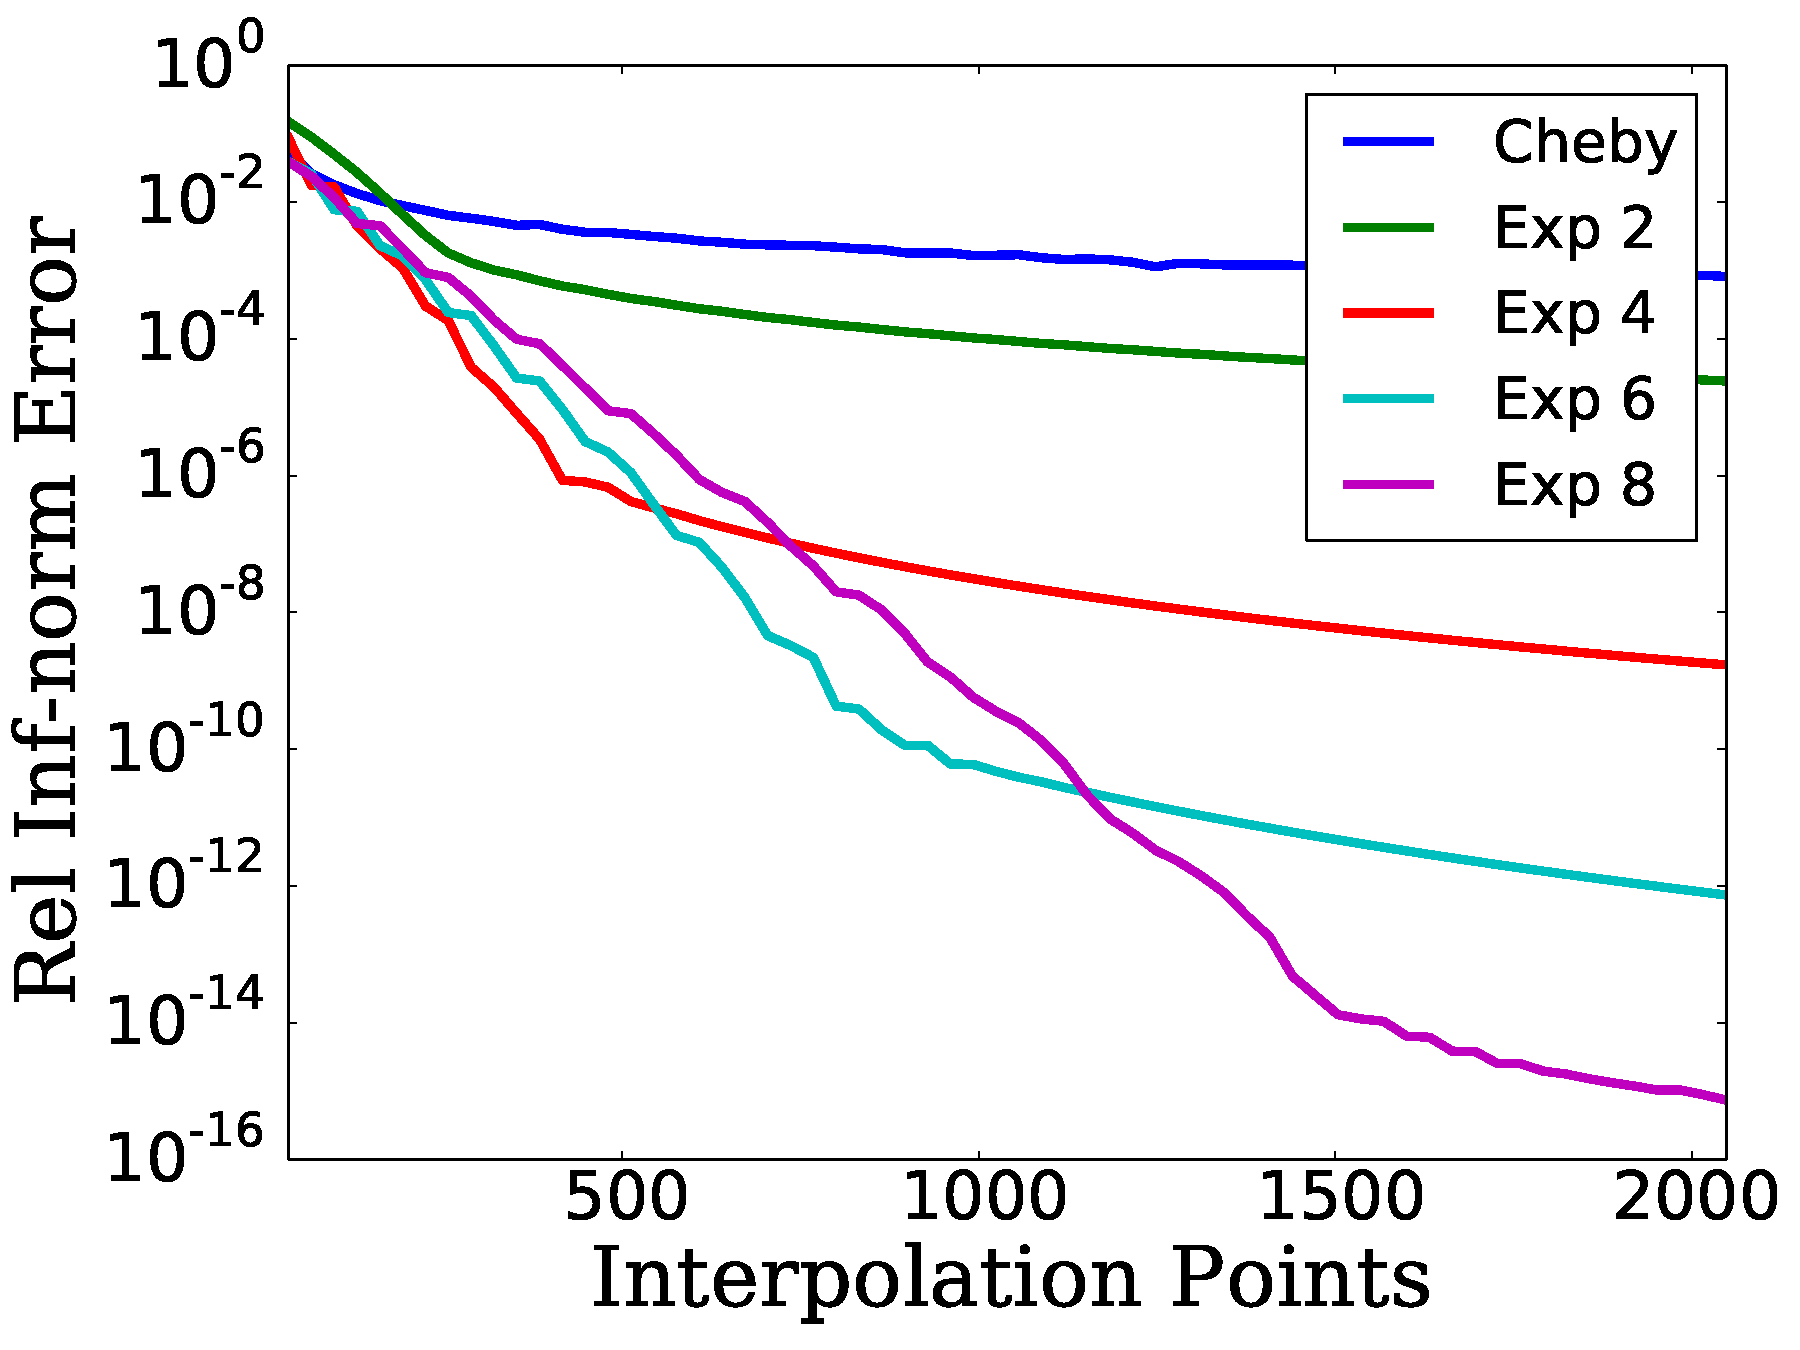
\includegraphics[width=\textwidth]{plots/cheby_interp_filter_2_rough_heaviside_2.pdf}
    \caption{Filters, Plot 2}
    \end{subfigure}
\caption[Rough Interpolation Comparison: Heaviside Jump Function 2]{
MSN interpolation and Chebyshev filtering results of the Heaviside jump
function $H_{2}$ for various $s$ values and filters.
We include standard Chebyshev interpolant in both filter examples for reference.
}
\label{fig:rough_comparison_heaviside_2}
\end{figure}




% Print results for comparing MSN with Heaviside jump function

\begin{figure}[p]
    \centering
    \begin{subfigure}{0.45\textwidth}
    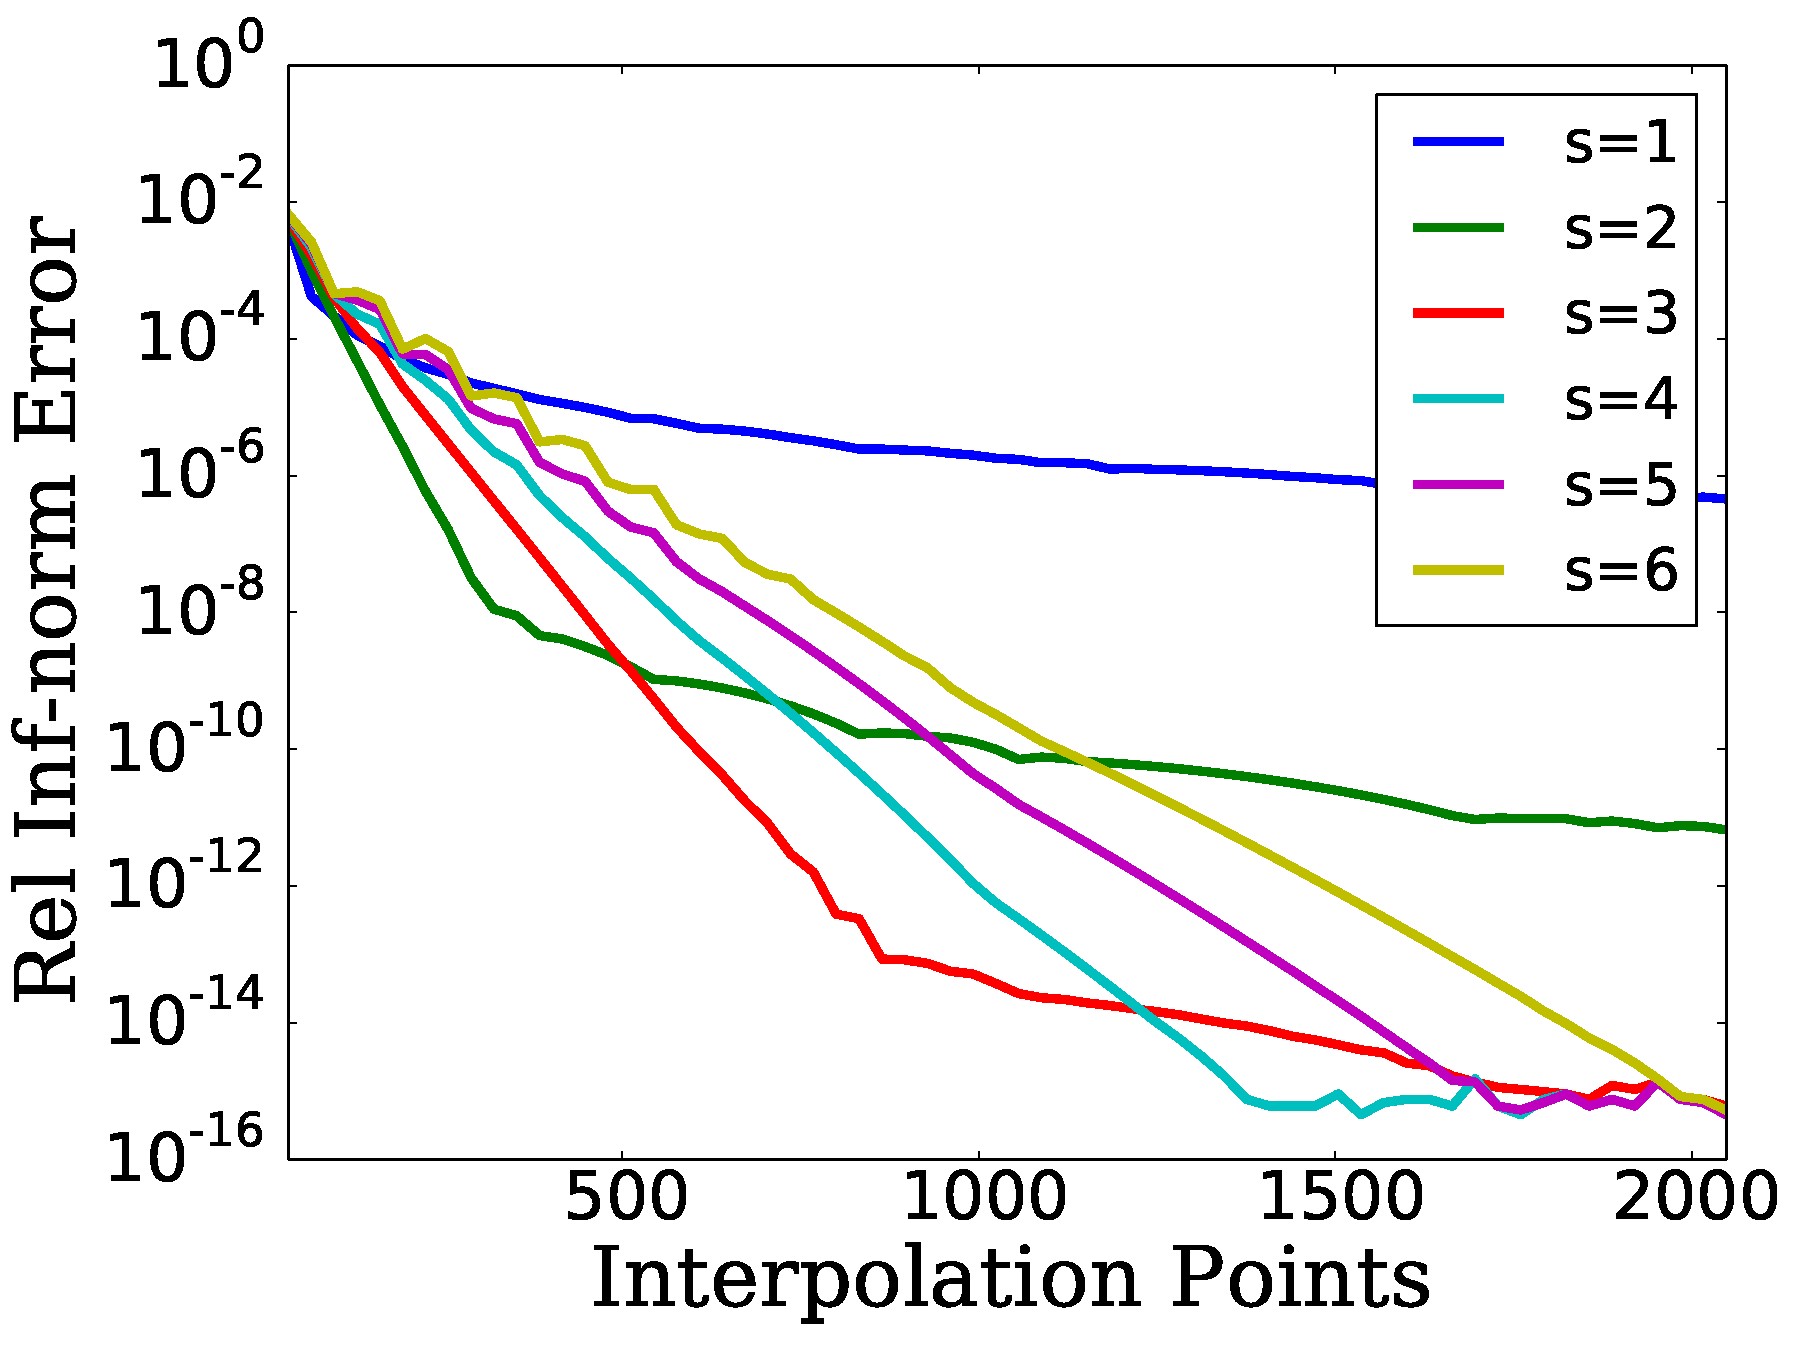
\includegraphics[width=\textwidth]{plots/msn_interp_fast_2n_rough_sharp_func_2.pdf}
    \caption{MSN Interpolation}
    \end{subfigure}

    \begin{subfigure}{0.45\textwidth}
    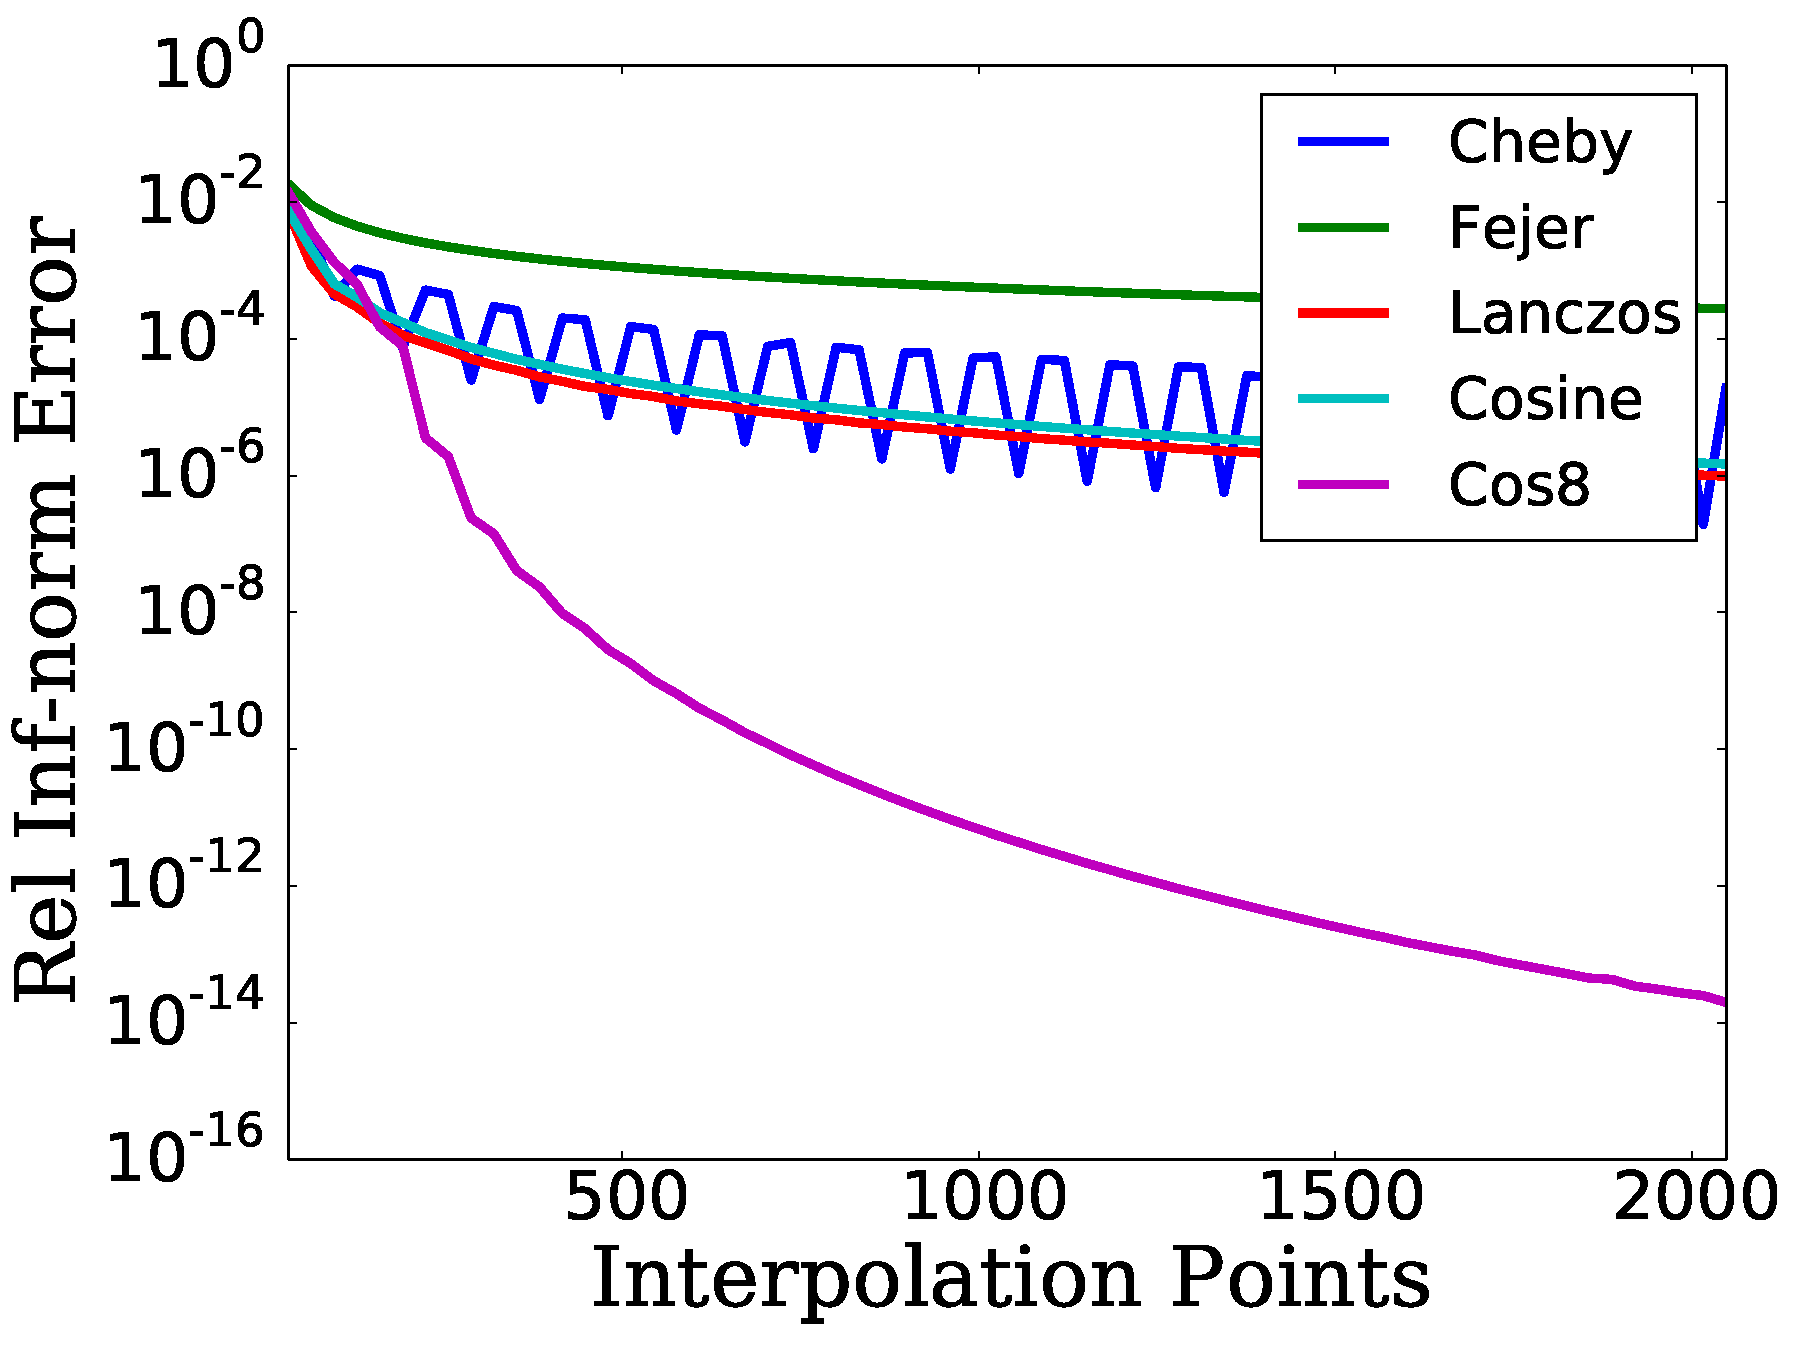
\includegraphics[width=\textwidth]{plots/cheby_interp_filter_rough_sharp_func_2.pdf}
    \caption{Filters, Plot 1}
    \end{subfigure}
    \begin{subfigure}{0.45\textwidth}
    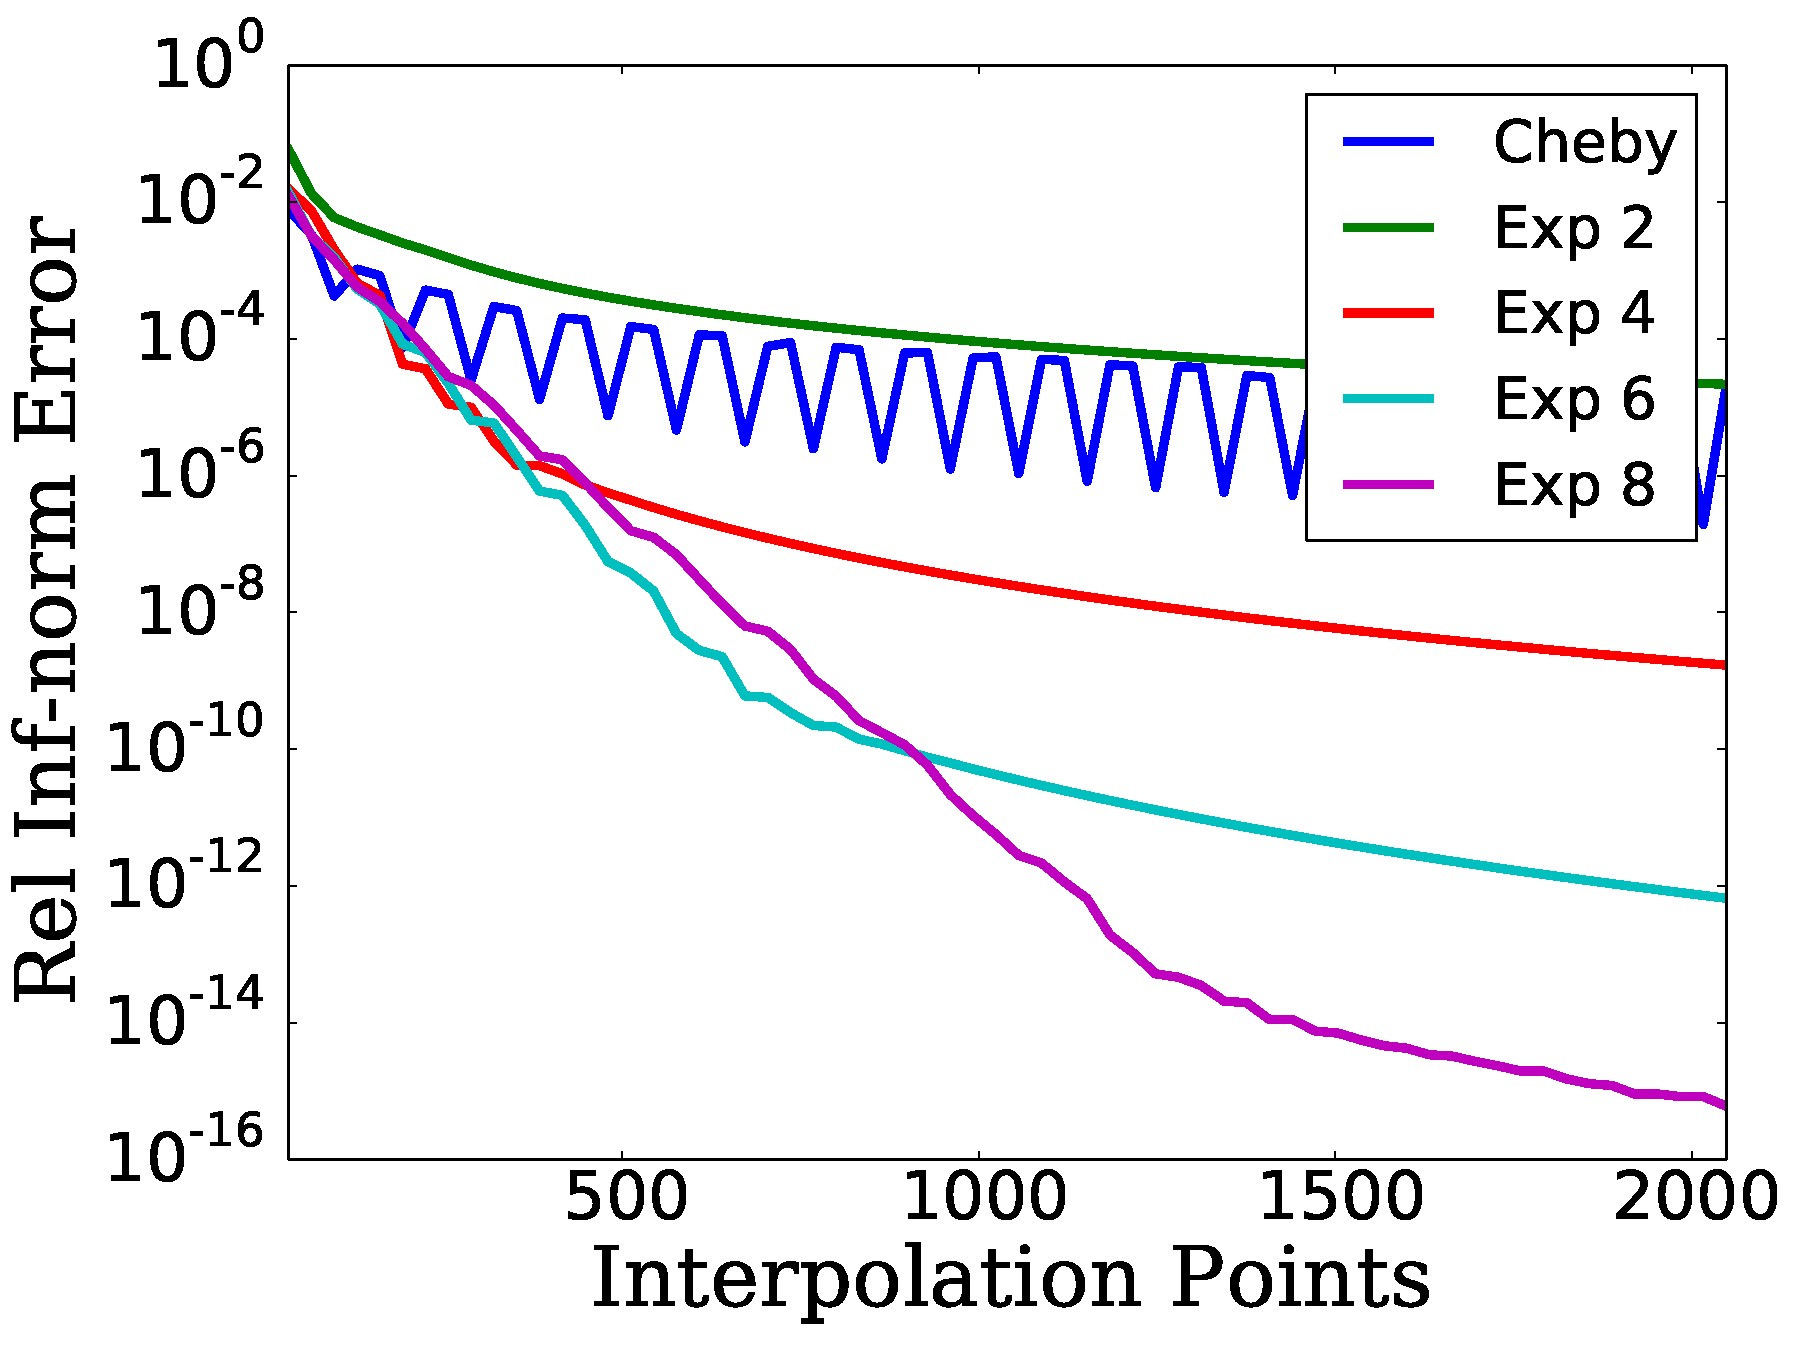
\includegraphics[width=\textwidth]{plots/cheby_interp_filter_2_rough_sharp_func_2.pdf}
    \caption{Filters, Plot 2}
    \end{subfigure}
\caption[Rough Interpolation Comparison: Sharp Function 2]{
MSN interpolation and Chebyshev filtering results of the Sharp Function
$G_{2}(\cdot,0.5)$ for various $s$ values and filters.
We include standard Chebyshev interpolant in both filter examples for reference.
}
\label{fig:rough_comparison_sharp_func_2}
\end{figure}




% Print results for comparing MSN with Heaviside jump function

\begin{figure}[p]
    \centering
    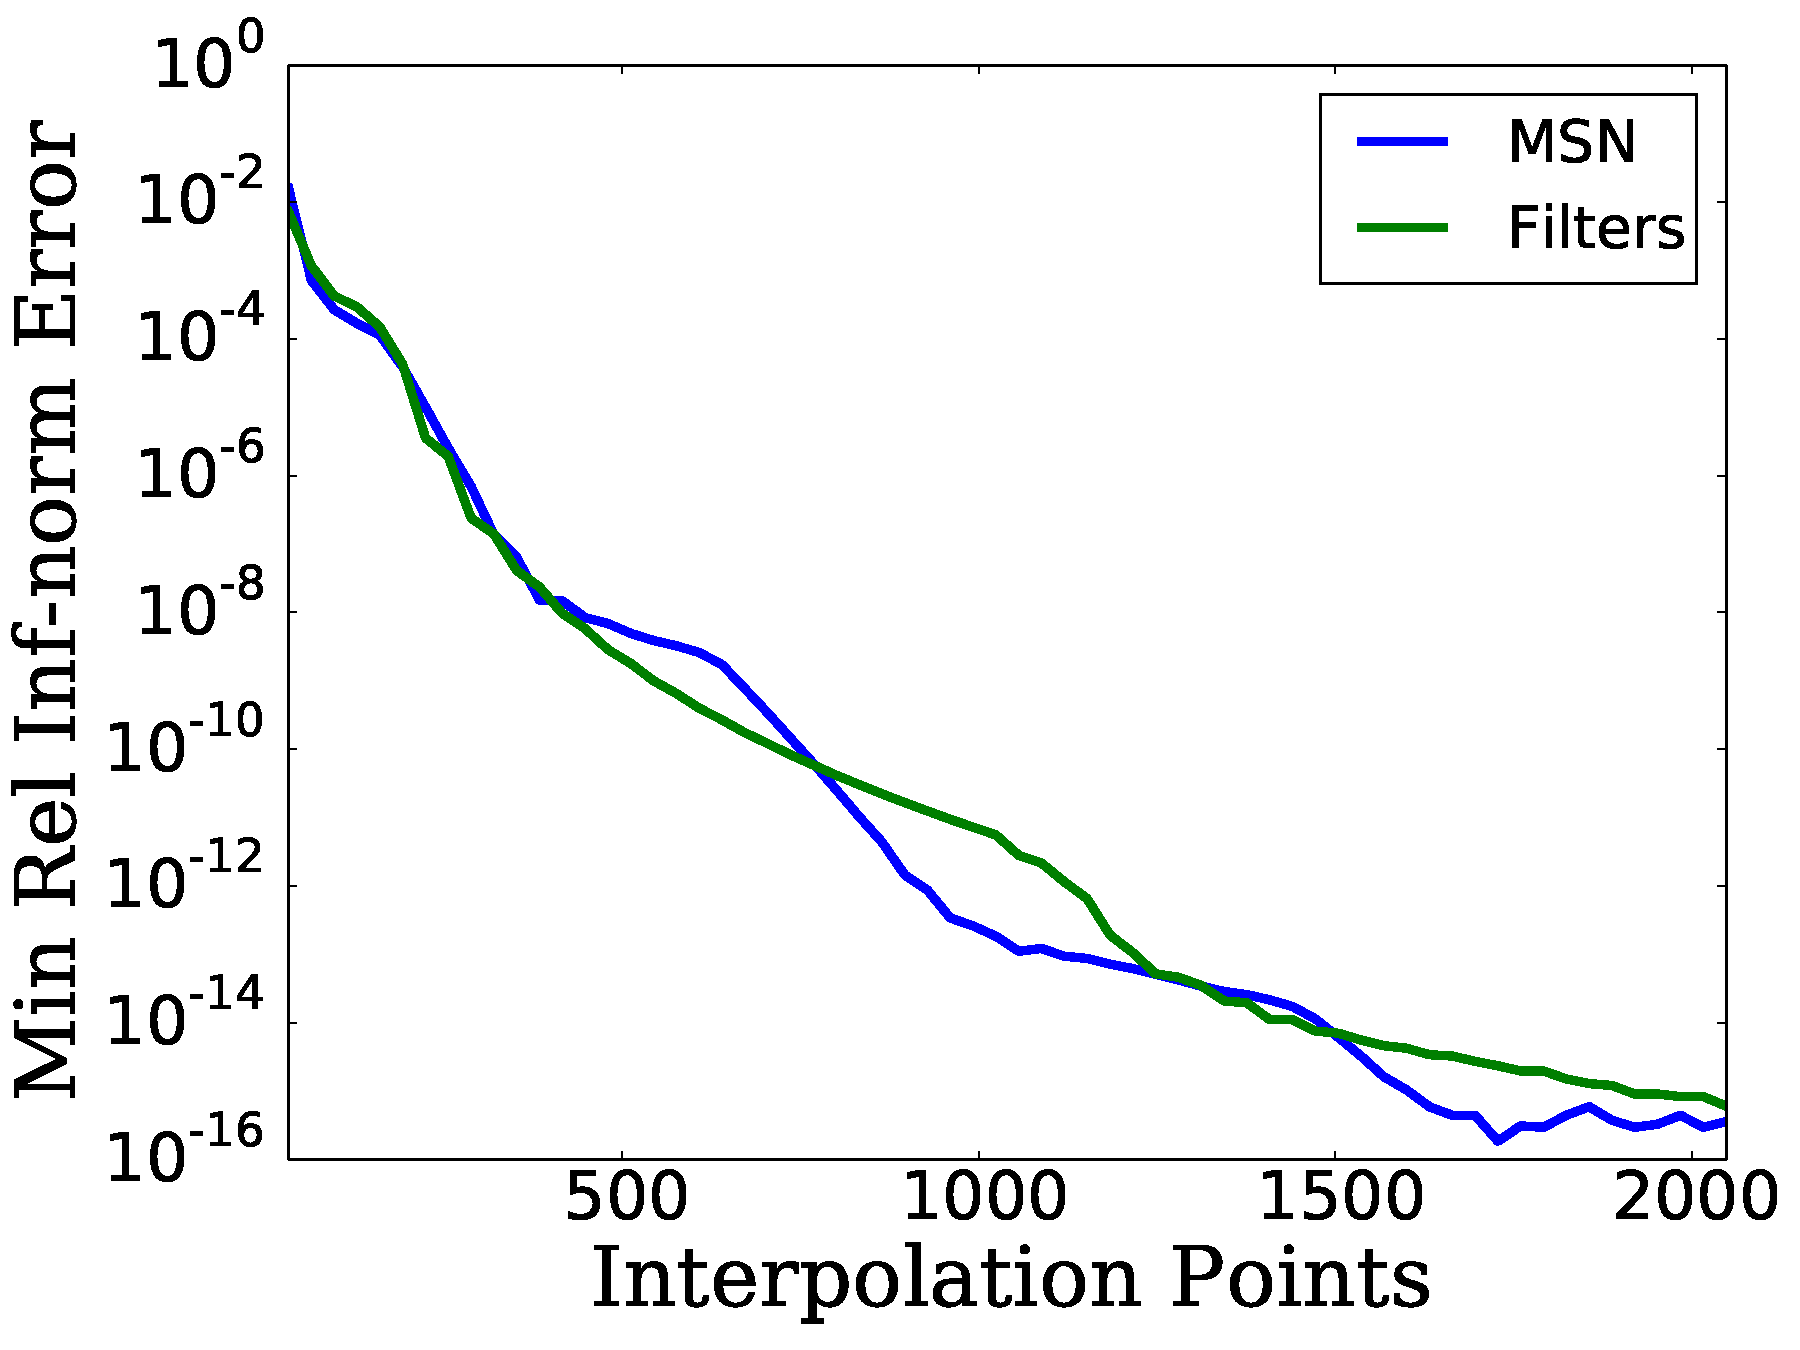
\includegraphics[width=0.9\textwidth]{plots/msn_filter_comp_heaviside_2.pdf}
    \caption[Best MSN vs.~Best Filter Comparison: Heaviside Jump Function 2]{
    We plot the minimum MSN interpolation error and compare it
    to the minimum filter error over all Chebshev filters.
    These error results are from attempting to approximate $H_{2}$.
    }
\label{fig:msn_filter_comp_heaviside_2}
\end{figure}




% Print results for comparing MSN with Heaviside jump function

\begin{figure}[p]
    \centering
    \begin{subfigure}{0.45\textwidth}
    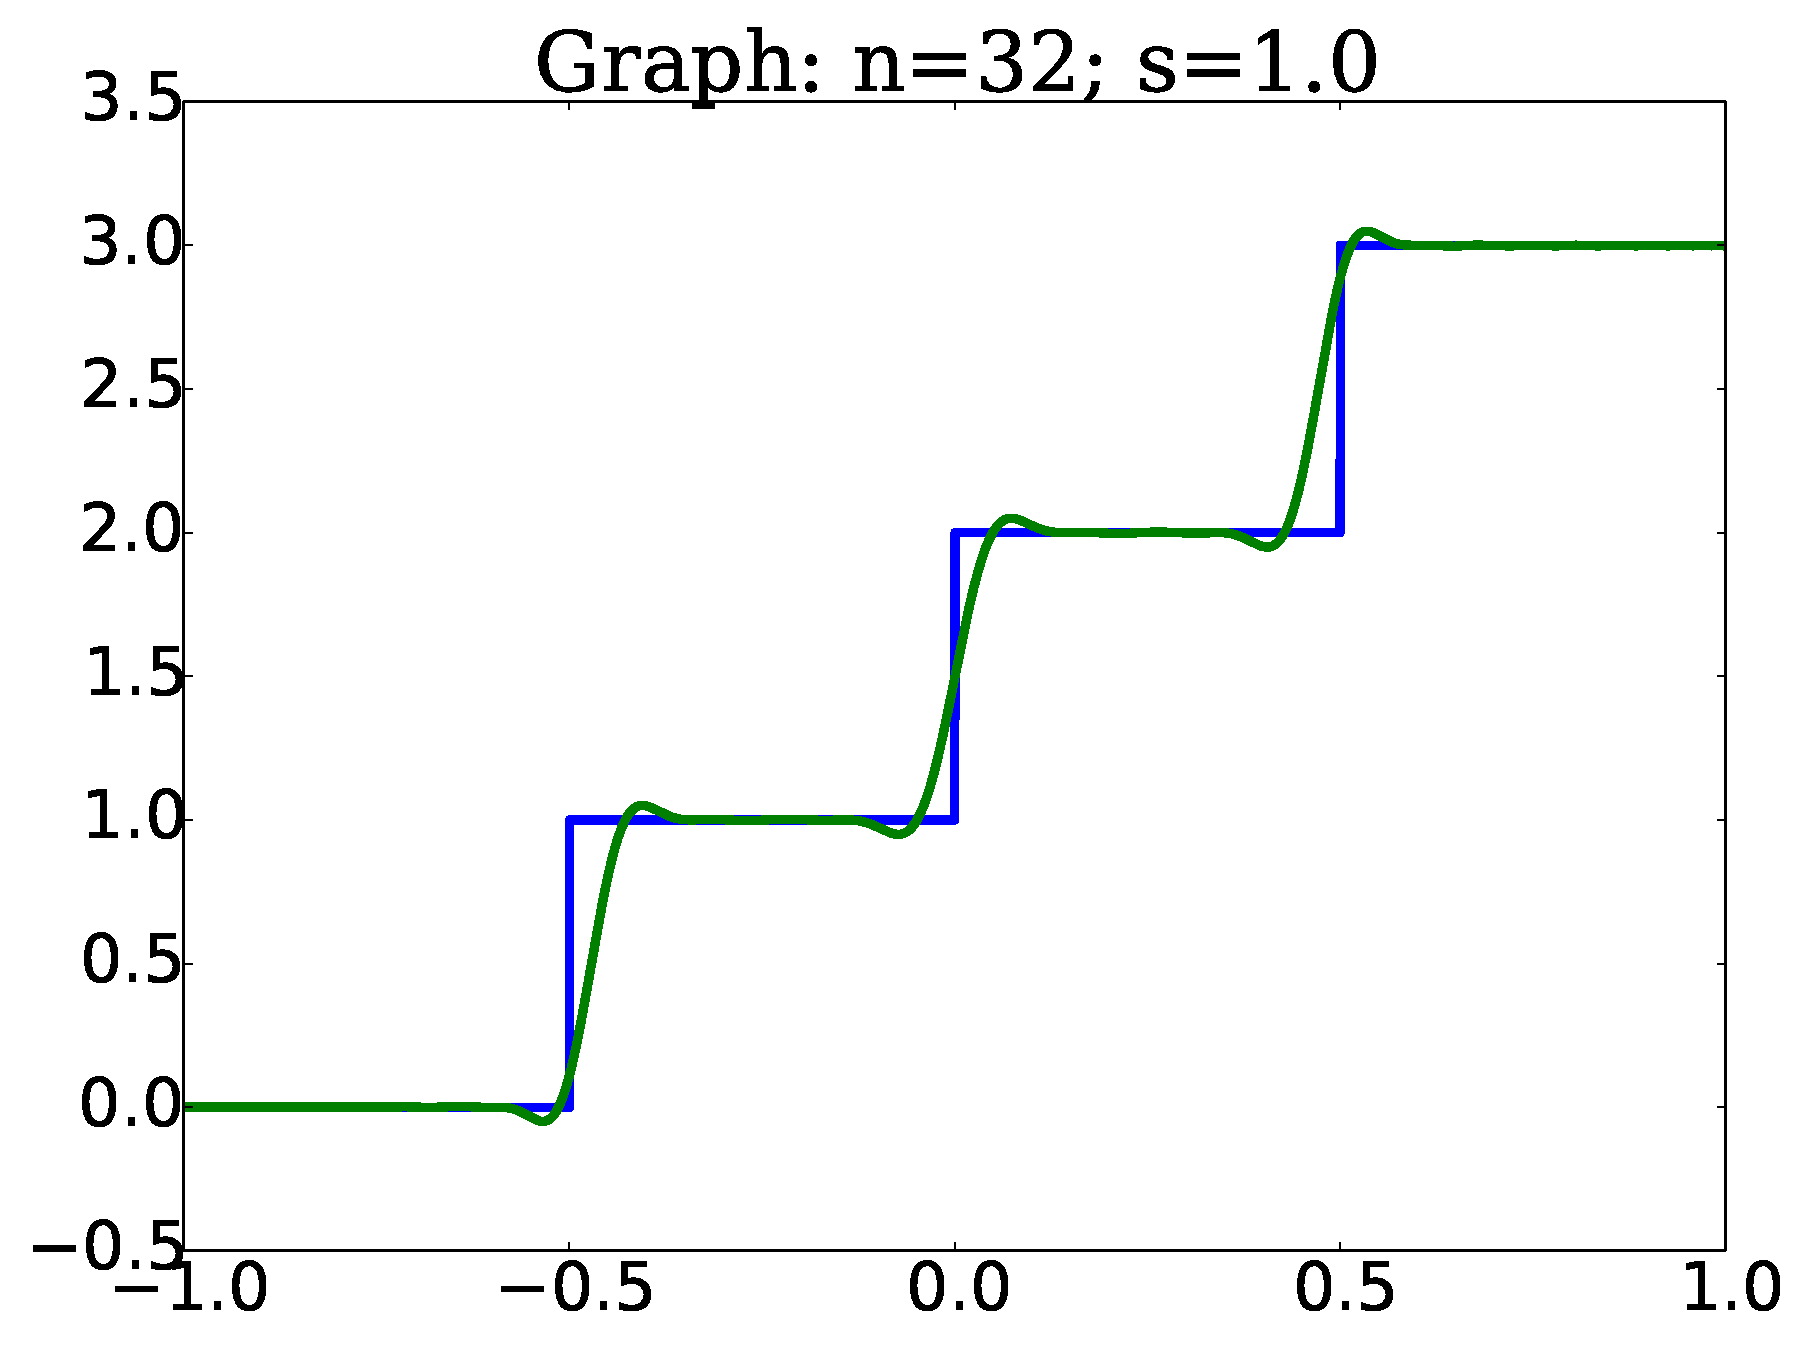
\includegraphics[width=\textwidth]{plots/graph_n_32_s_1_heaviside_2.pdf}
    \end{subfigure}
    \begin{subfigure}{0.45\textwidth}
    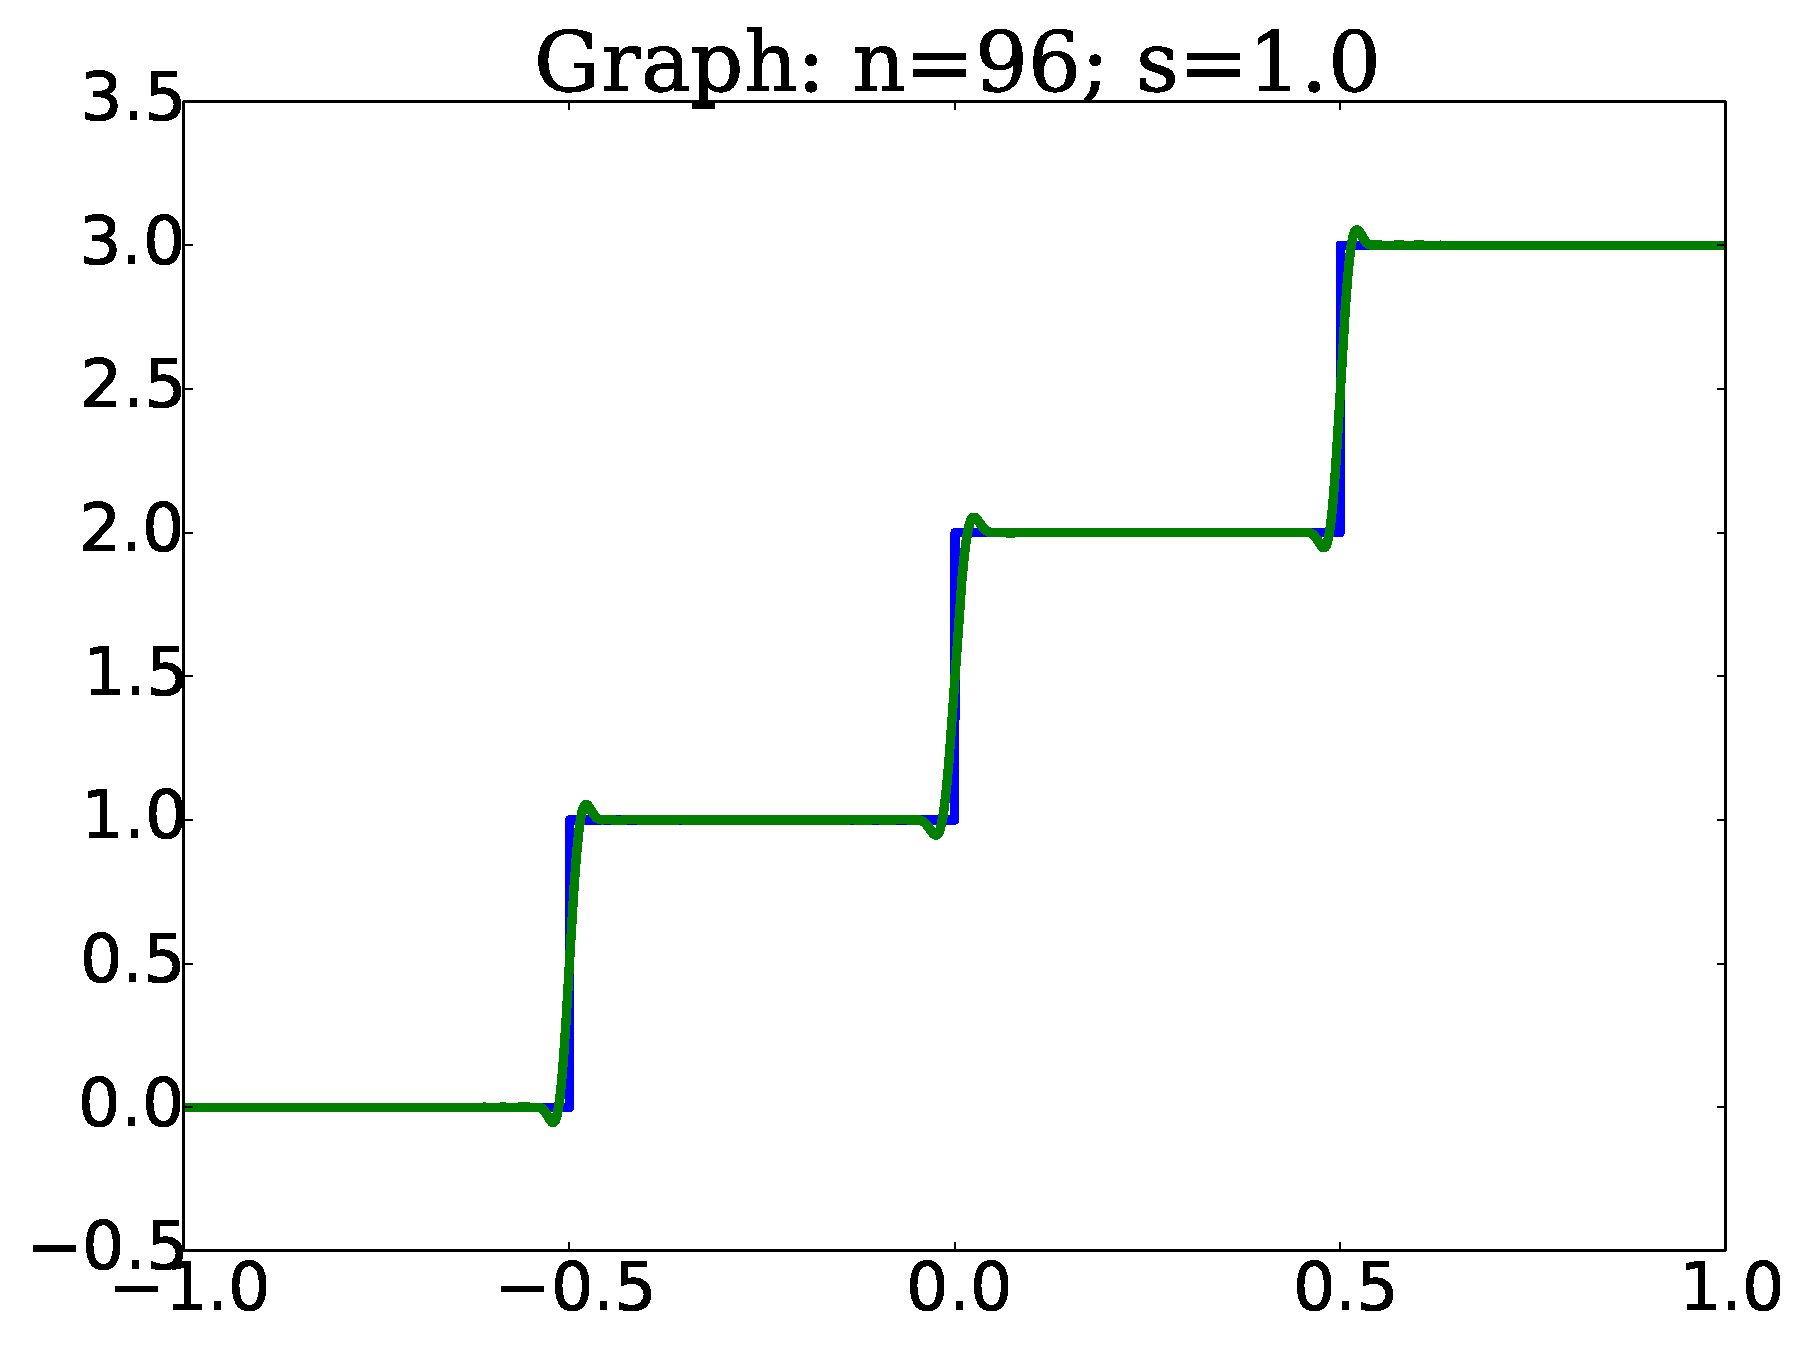
\includegraphics[width=\textwidth]{plots/graph_n_96_s_1_heaviside_2.pdf}
    \end{subfigure}

    \begin{subfigure}{0.45\textwidth}
    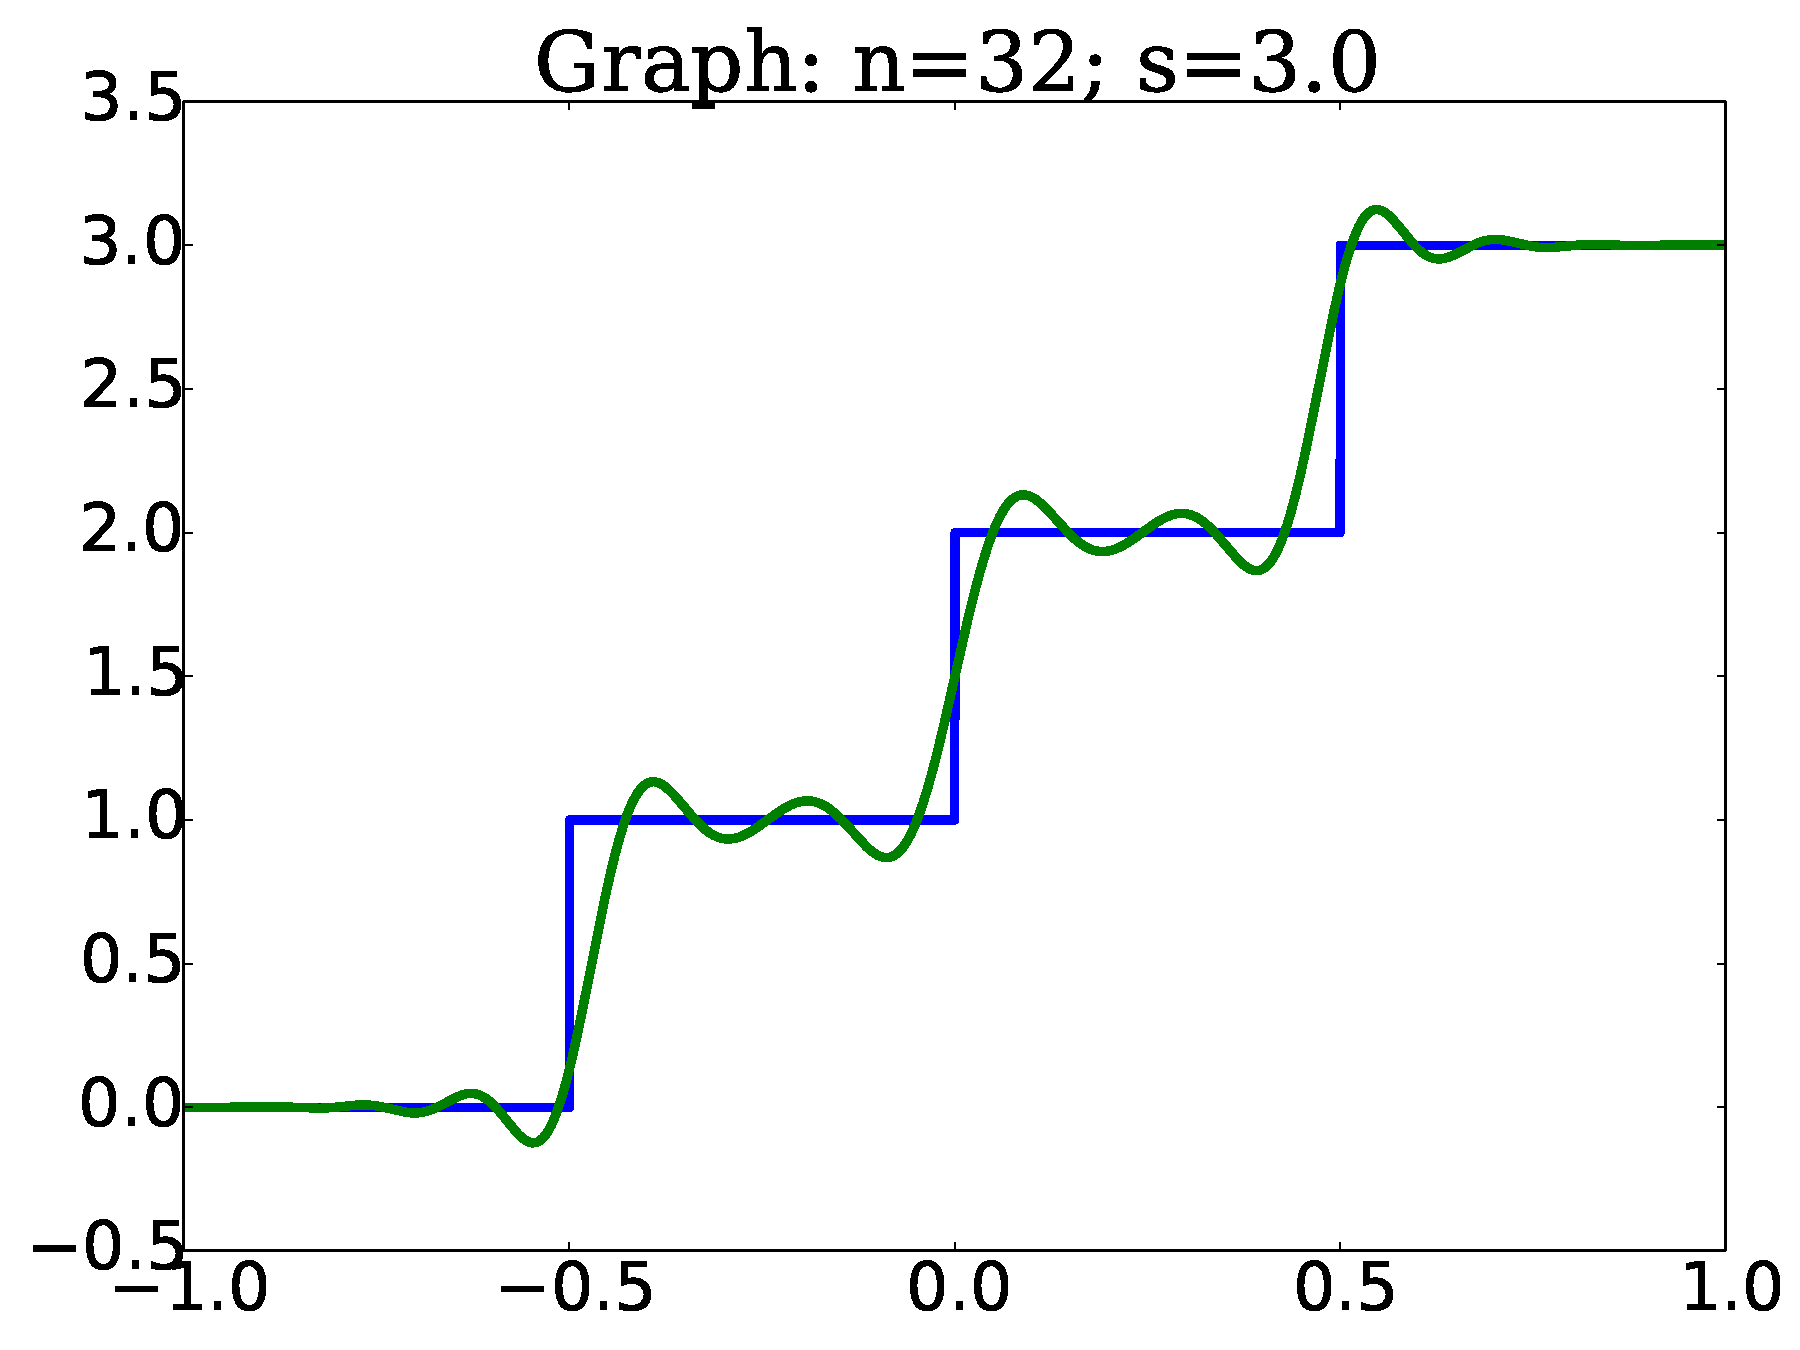
\includegraphics[width=\textwidth]{plots/graph_n_32_s_3_heaviside_2.pdf}
    \end{subfigure}
    \begin{subfigure}{0.45\textwidth}
    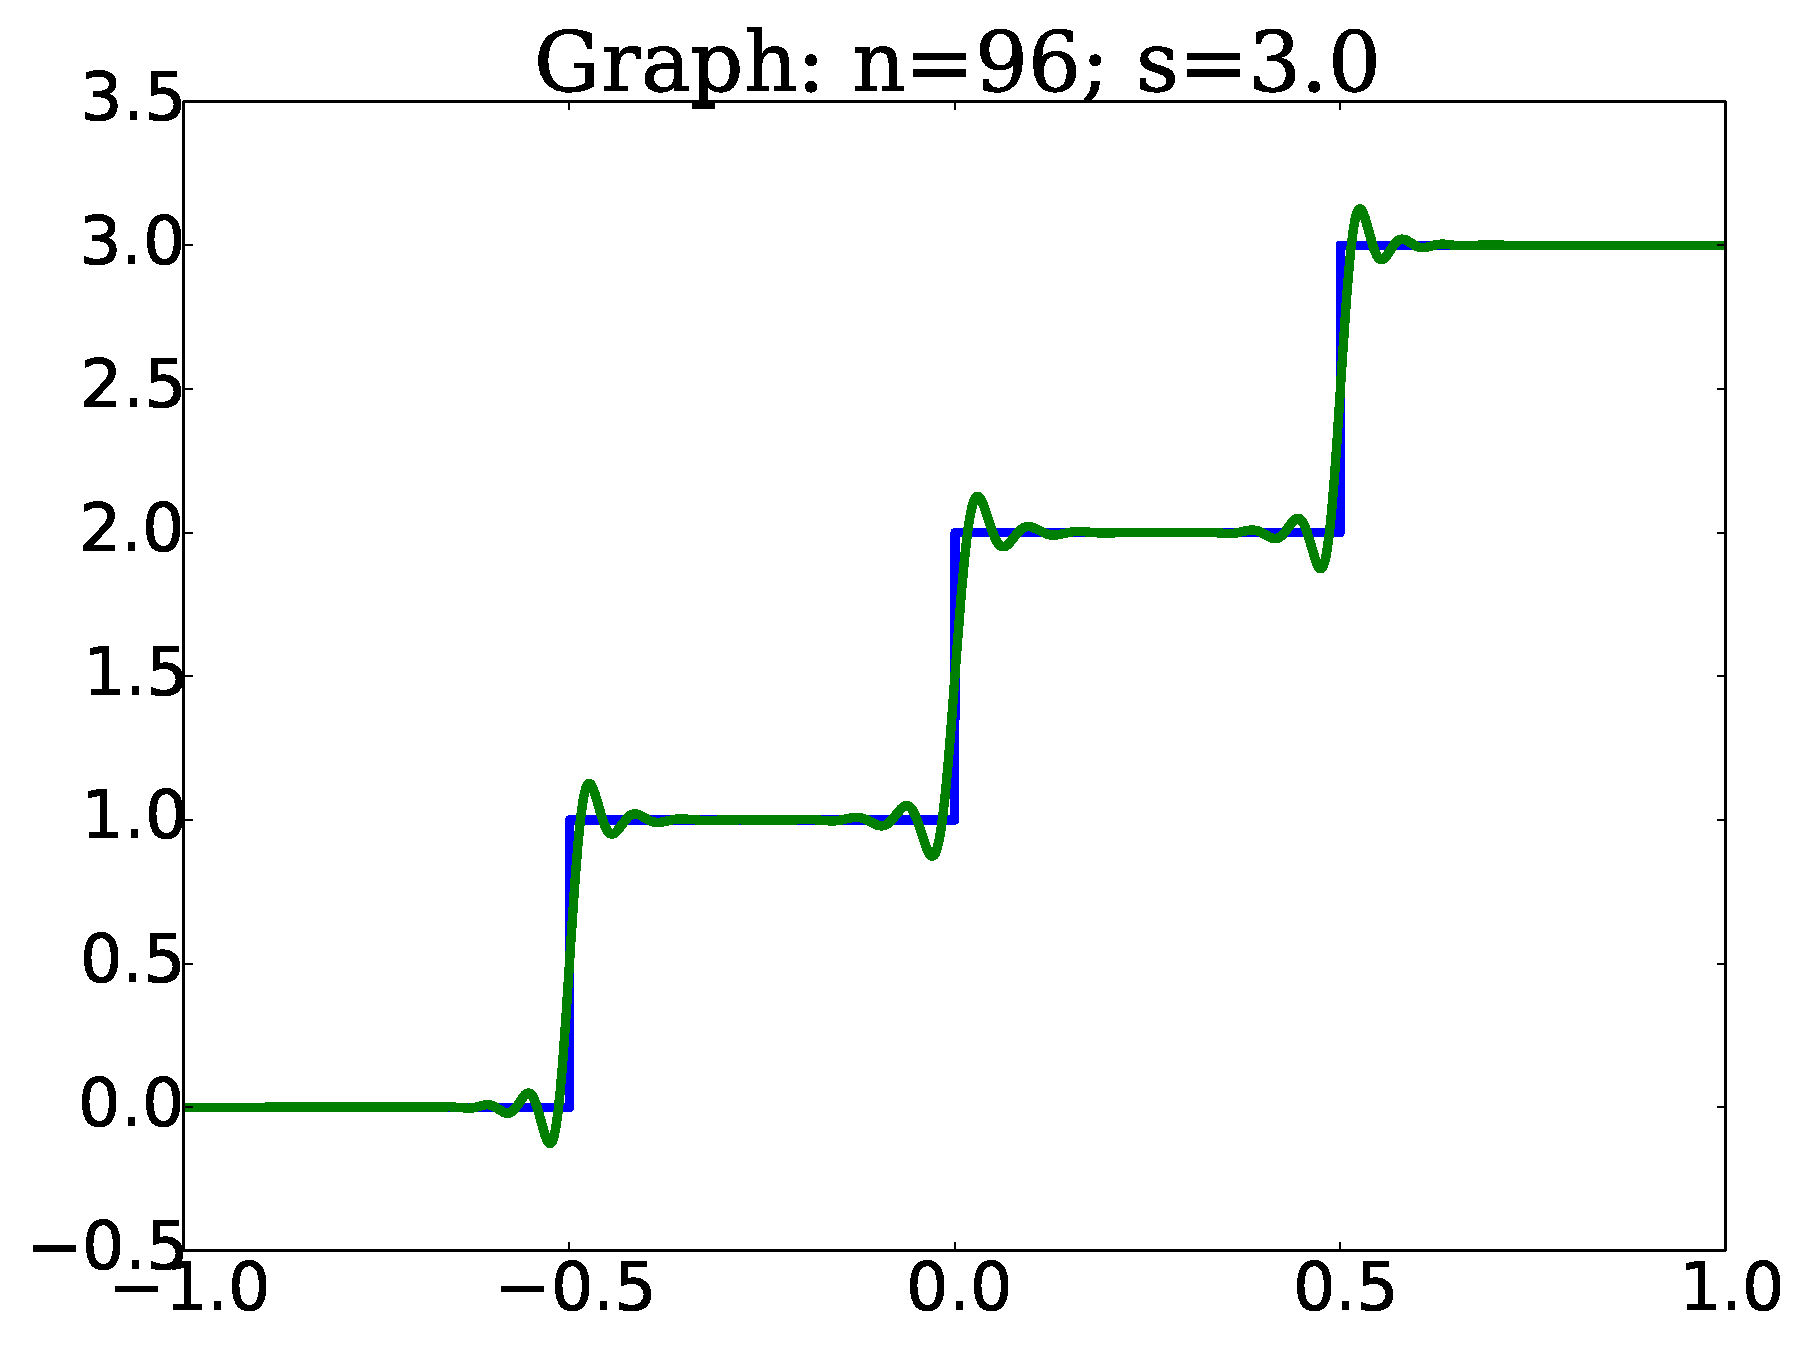
\includegraphics[width=\textwidth]{plots/graph_n_96_s_3_heaviside_2.pdf}
    \end{subfigure}

    \begin{subfigure}{0.45\textwidth}
    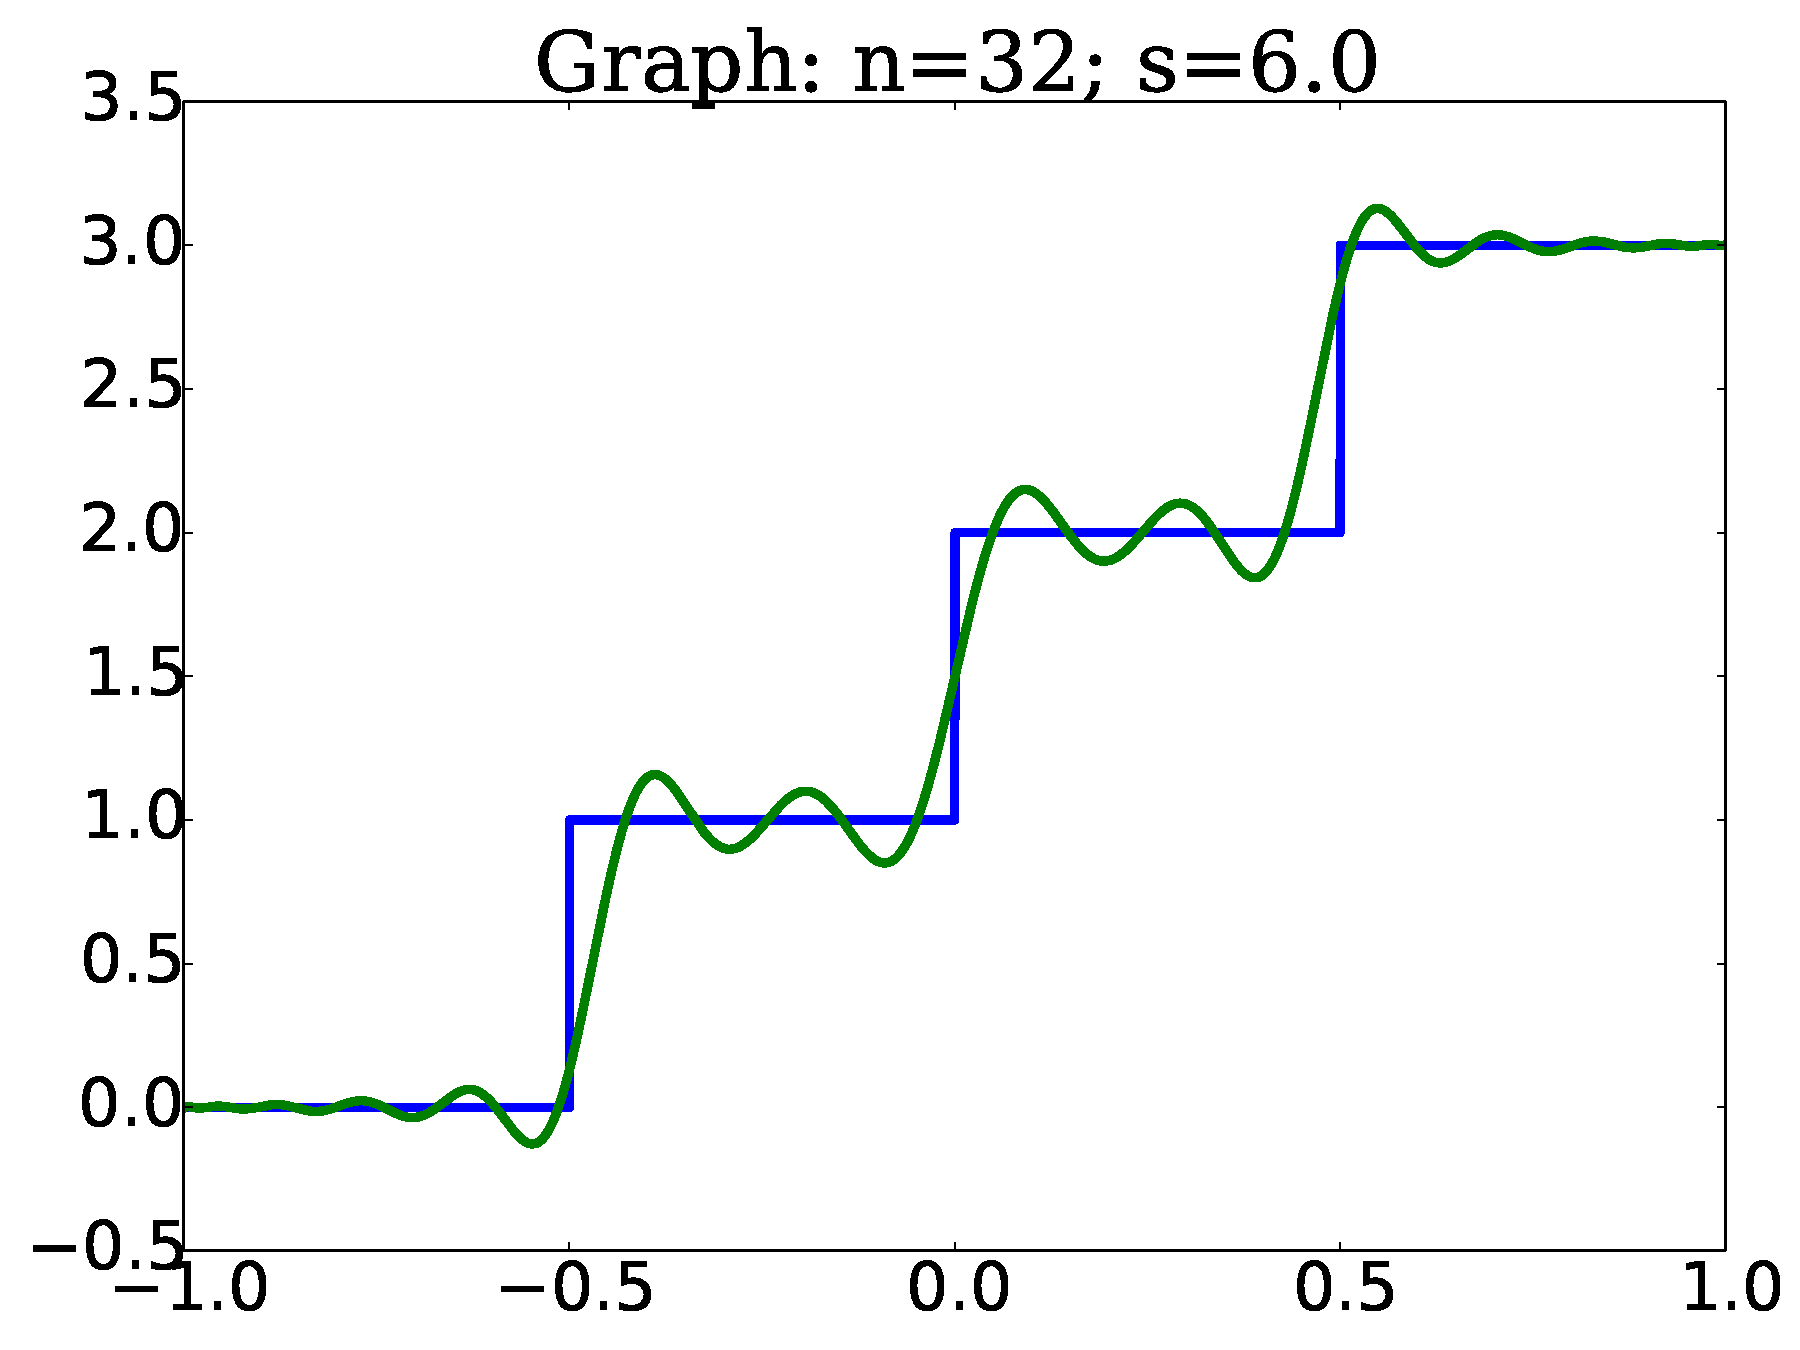
\includegraphics[width=\textwidth]{plots/graph_n_32_s_6_heaviside_2.pdf}
    \end{subfigure}
    \begin{subfigure}{0.45\textwidth}
    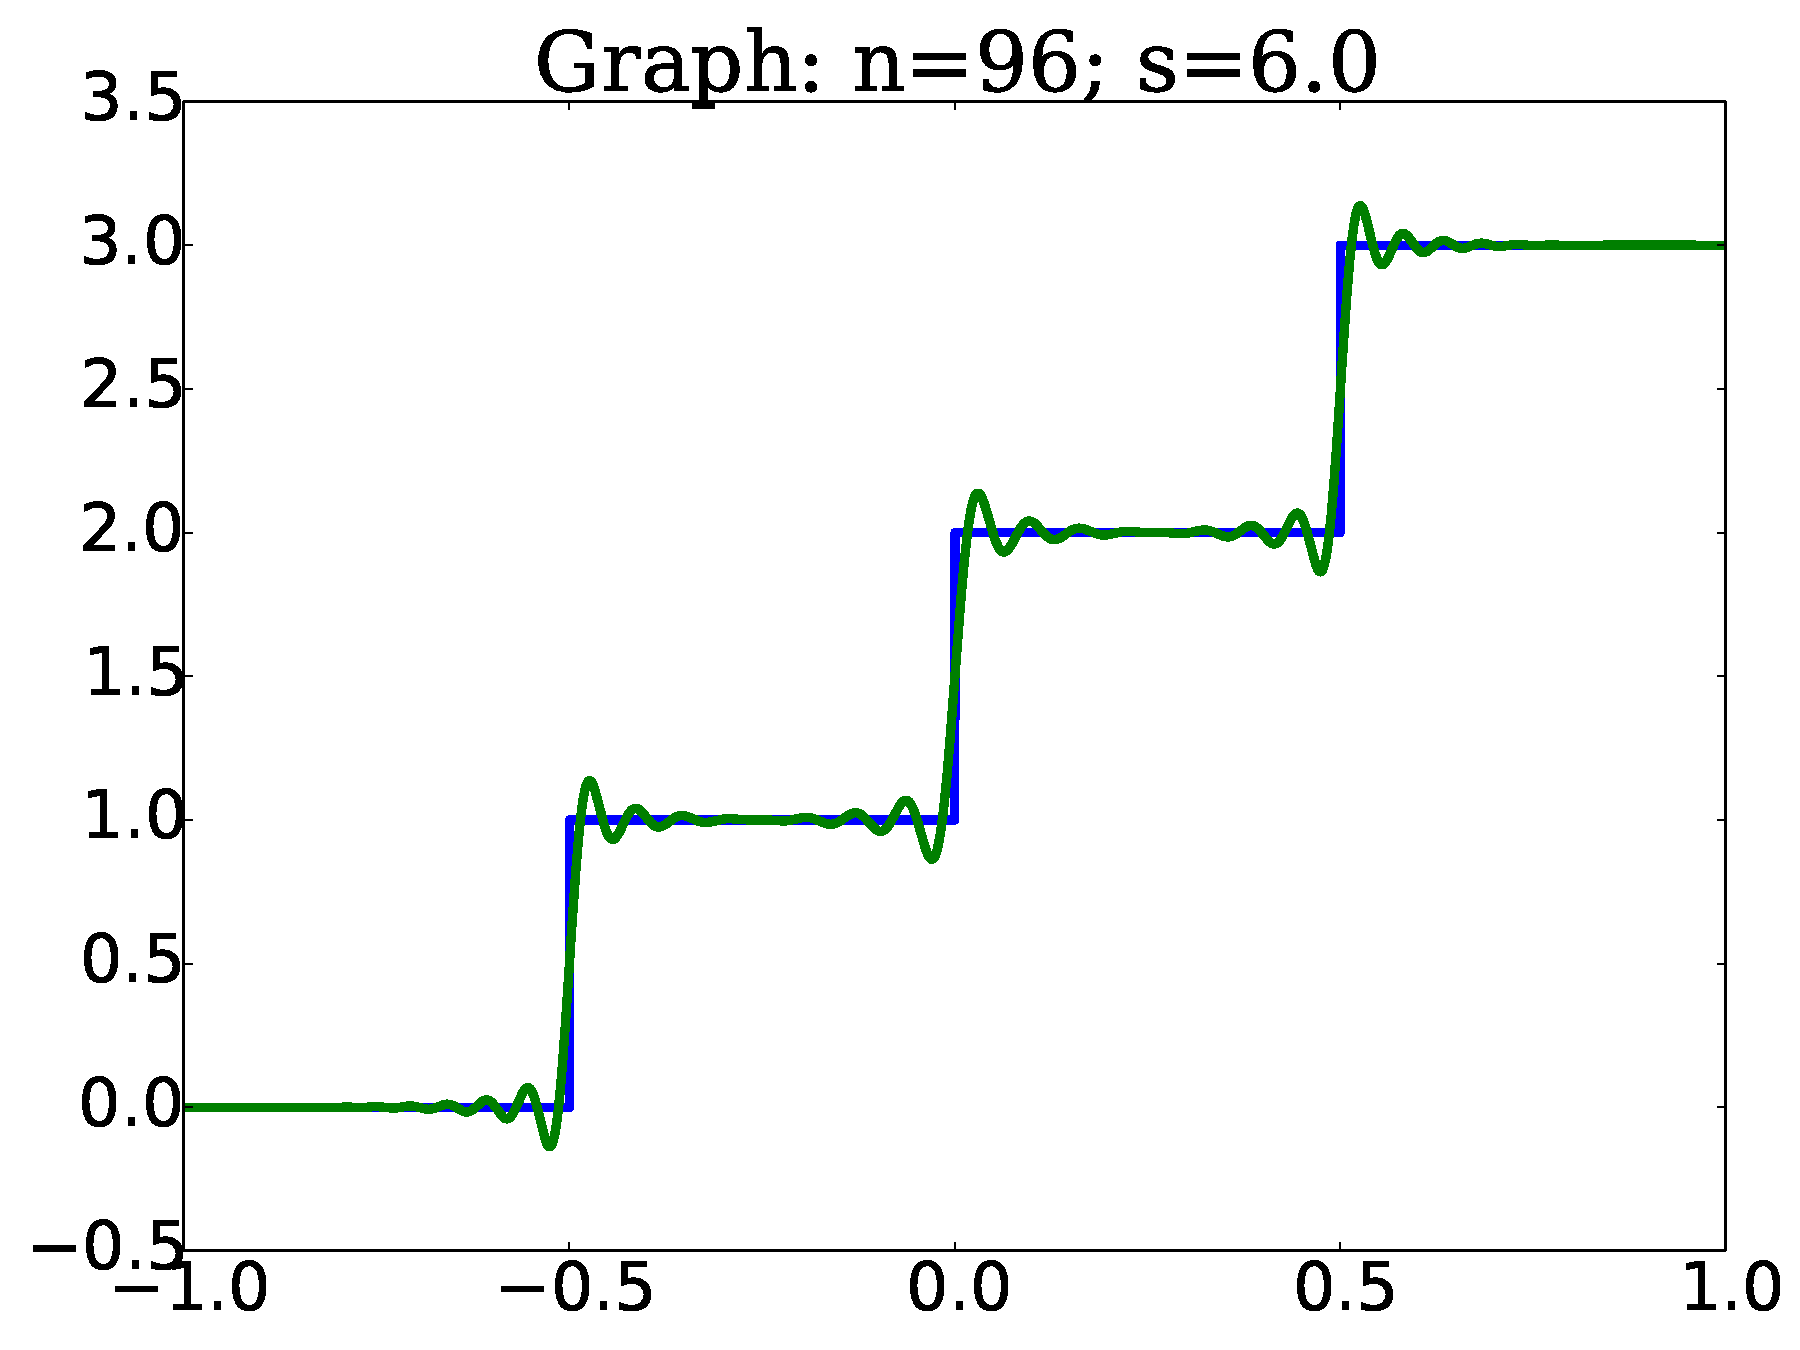
\includegraphics[width=\textwidth]{plots/graph_n_96_s_6_heaviside_2.pdf}
    \end{subfigure}
\caption[Example Plots of MSN Interpolation of Rough Functions]{
We plot MSN approximations against the true solution $H_{2}$
for various $s$ and $n$ values.
}
\label{fig:msn_n_s_heaviside_2}
\end{figure}




% Print results for comparing MSN with Heaviside jump function

\begin{figure}[p]
    \centering
    \begin{subfigure}{0.45\textwidth}
    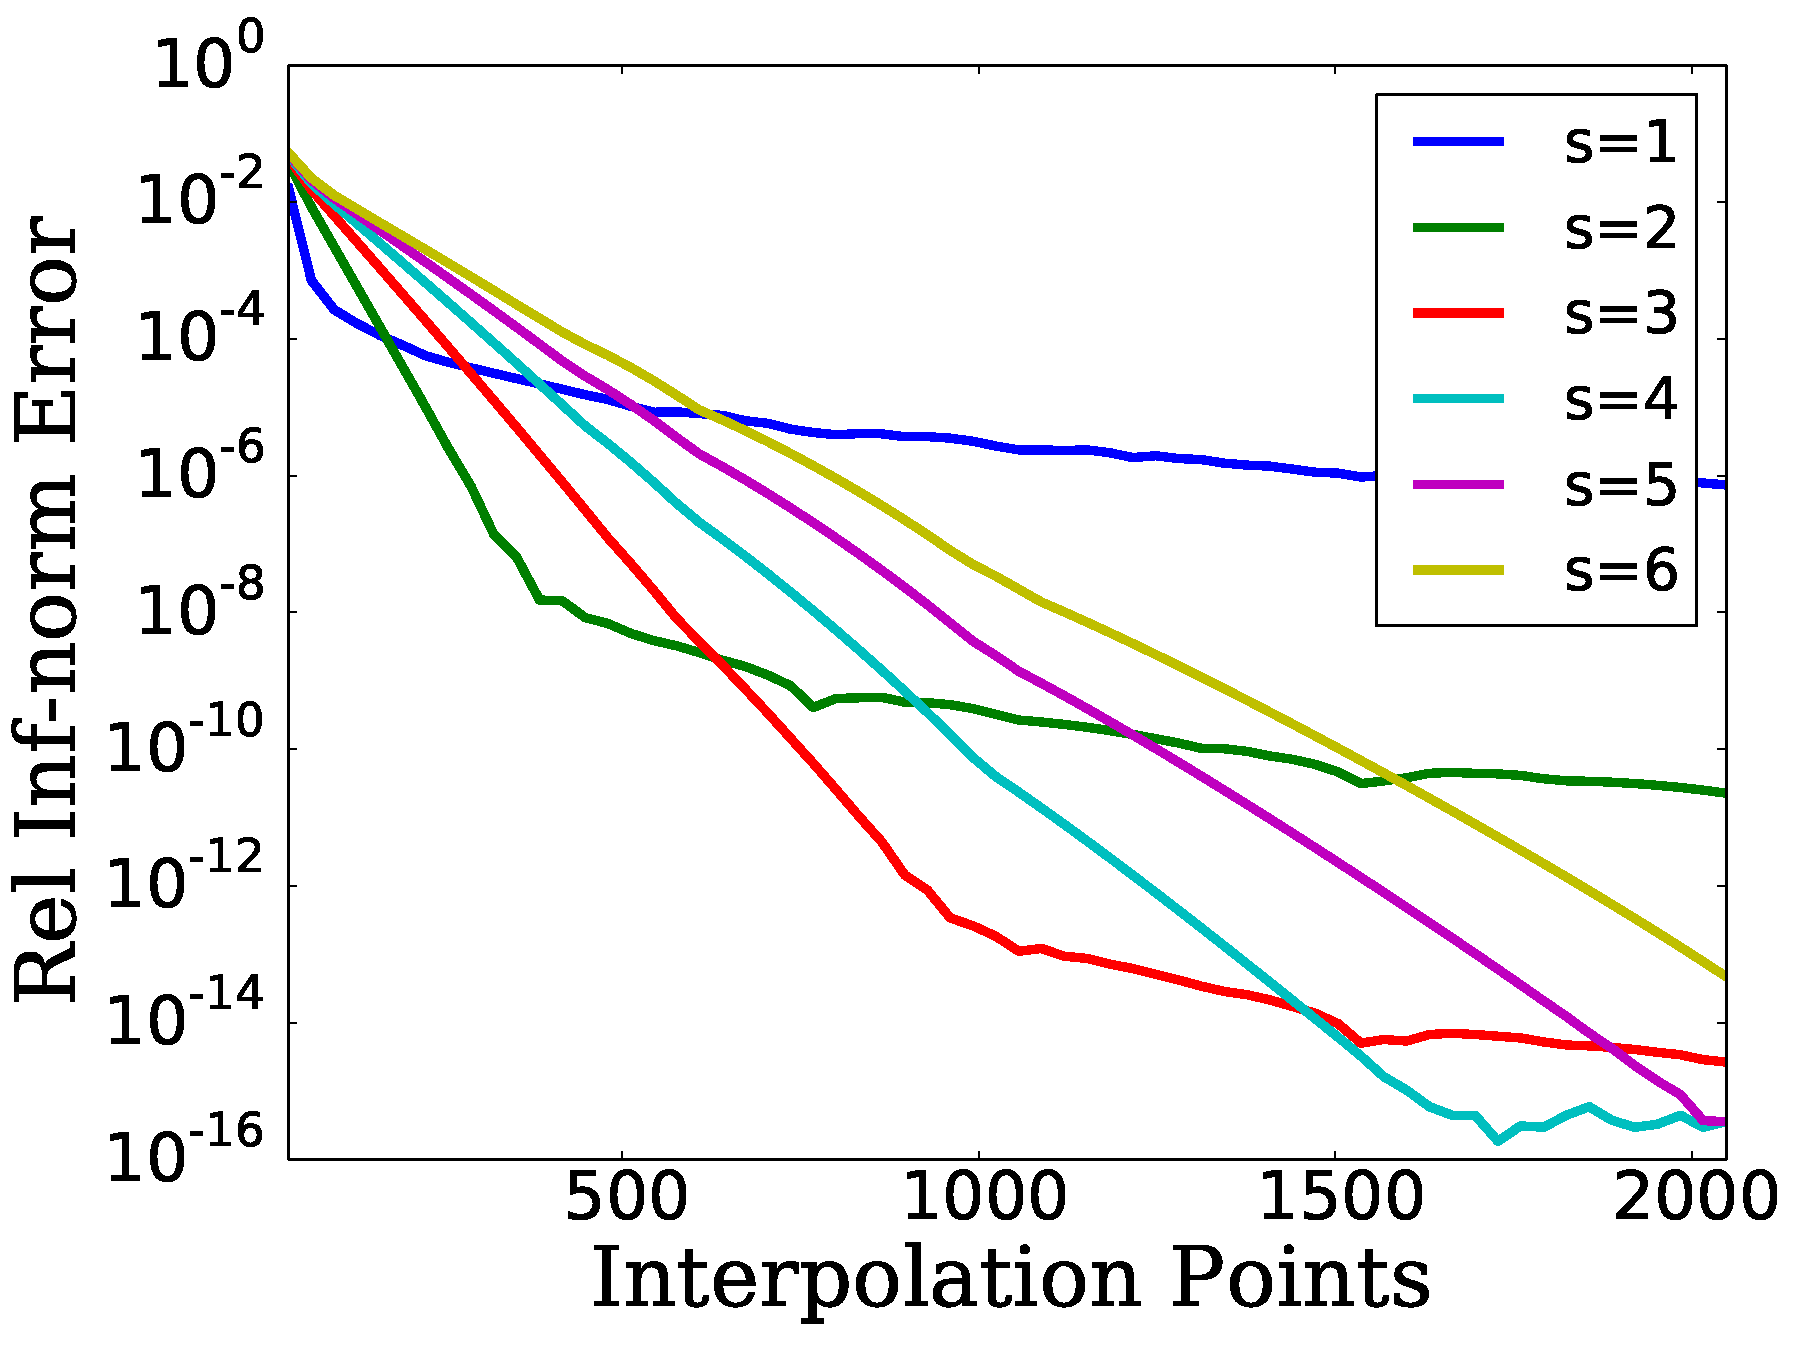
\includegraphics[width=\textwidth]{plots/msn_interp_fast_2n_rough_heaviside_2.pdf}
    \caption{Degree $2n$}
    \end{subfigure}
    \begin{subfigure}{0.45\textwidth}
    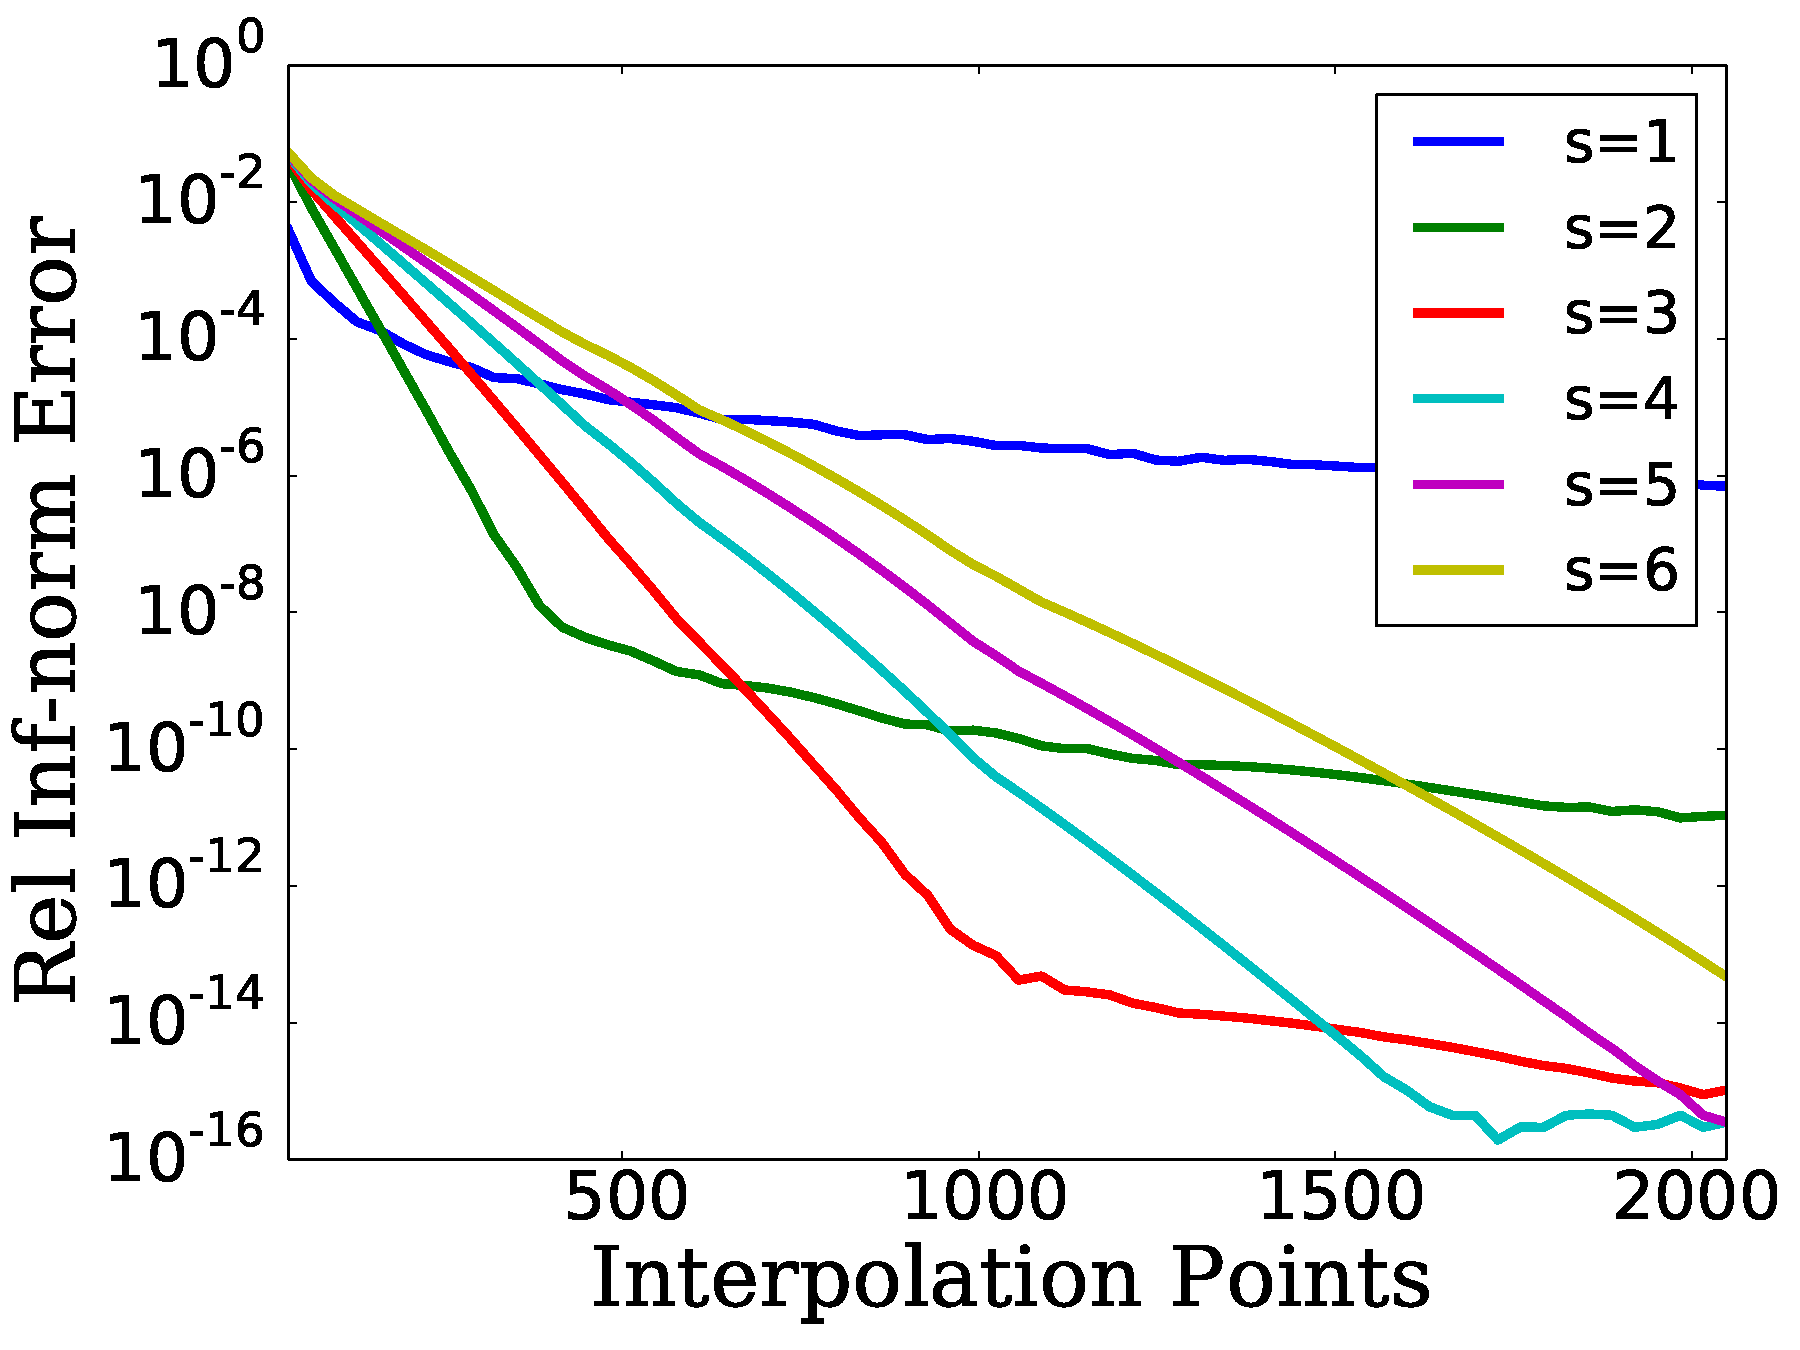
\includegraphics[width=\textwidth]{plots/msn_interp_fast_4n_rough_heaviside_2.pdf}
    \caption{Degree $4n$}
    \end{subfigure}

    \begin{subfigure}{0.45\textwidth}
    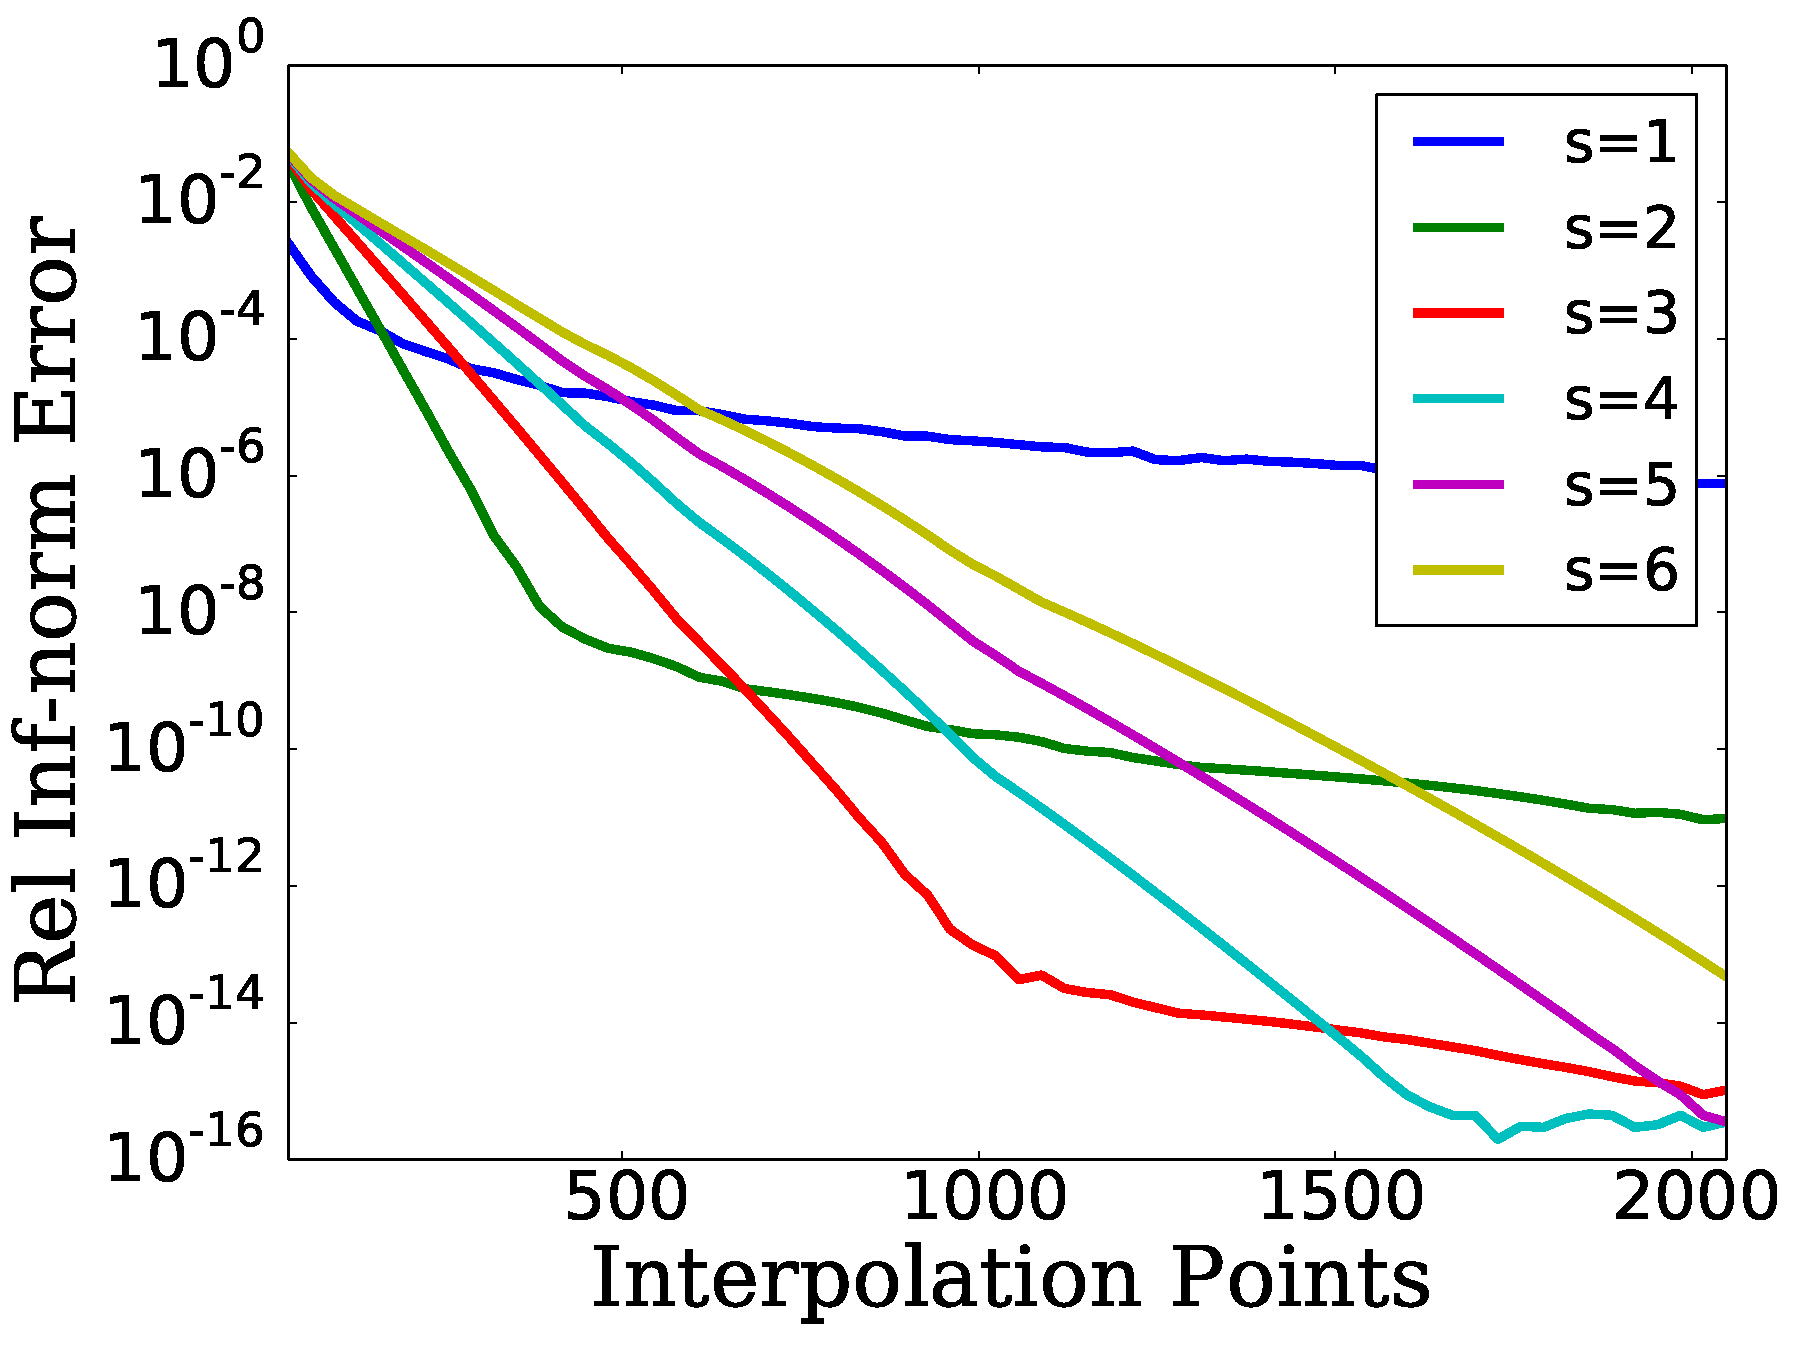
\includegraphics[width=\textwidth]{plots/msn_interp_fast_6n_rough_heaviside_2.pdf}
    \caption{Degree $6n$}
    \end{subfigure}
    \begin{subfigure}{0.45\textwidth}
    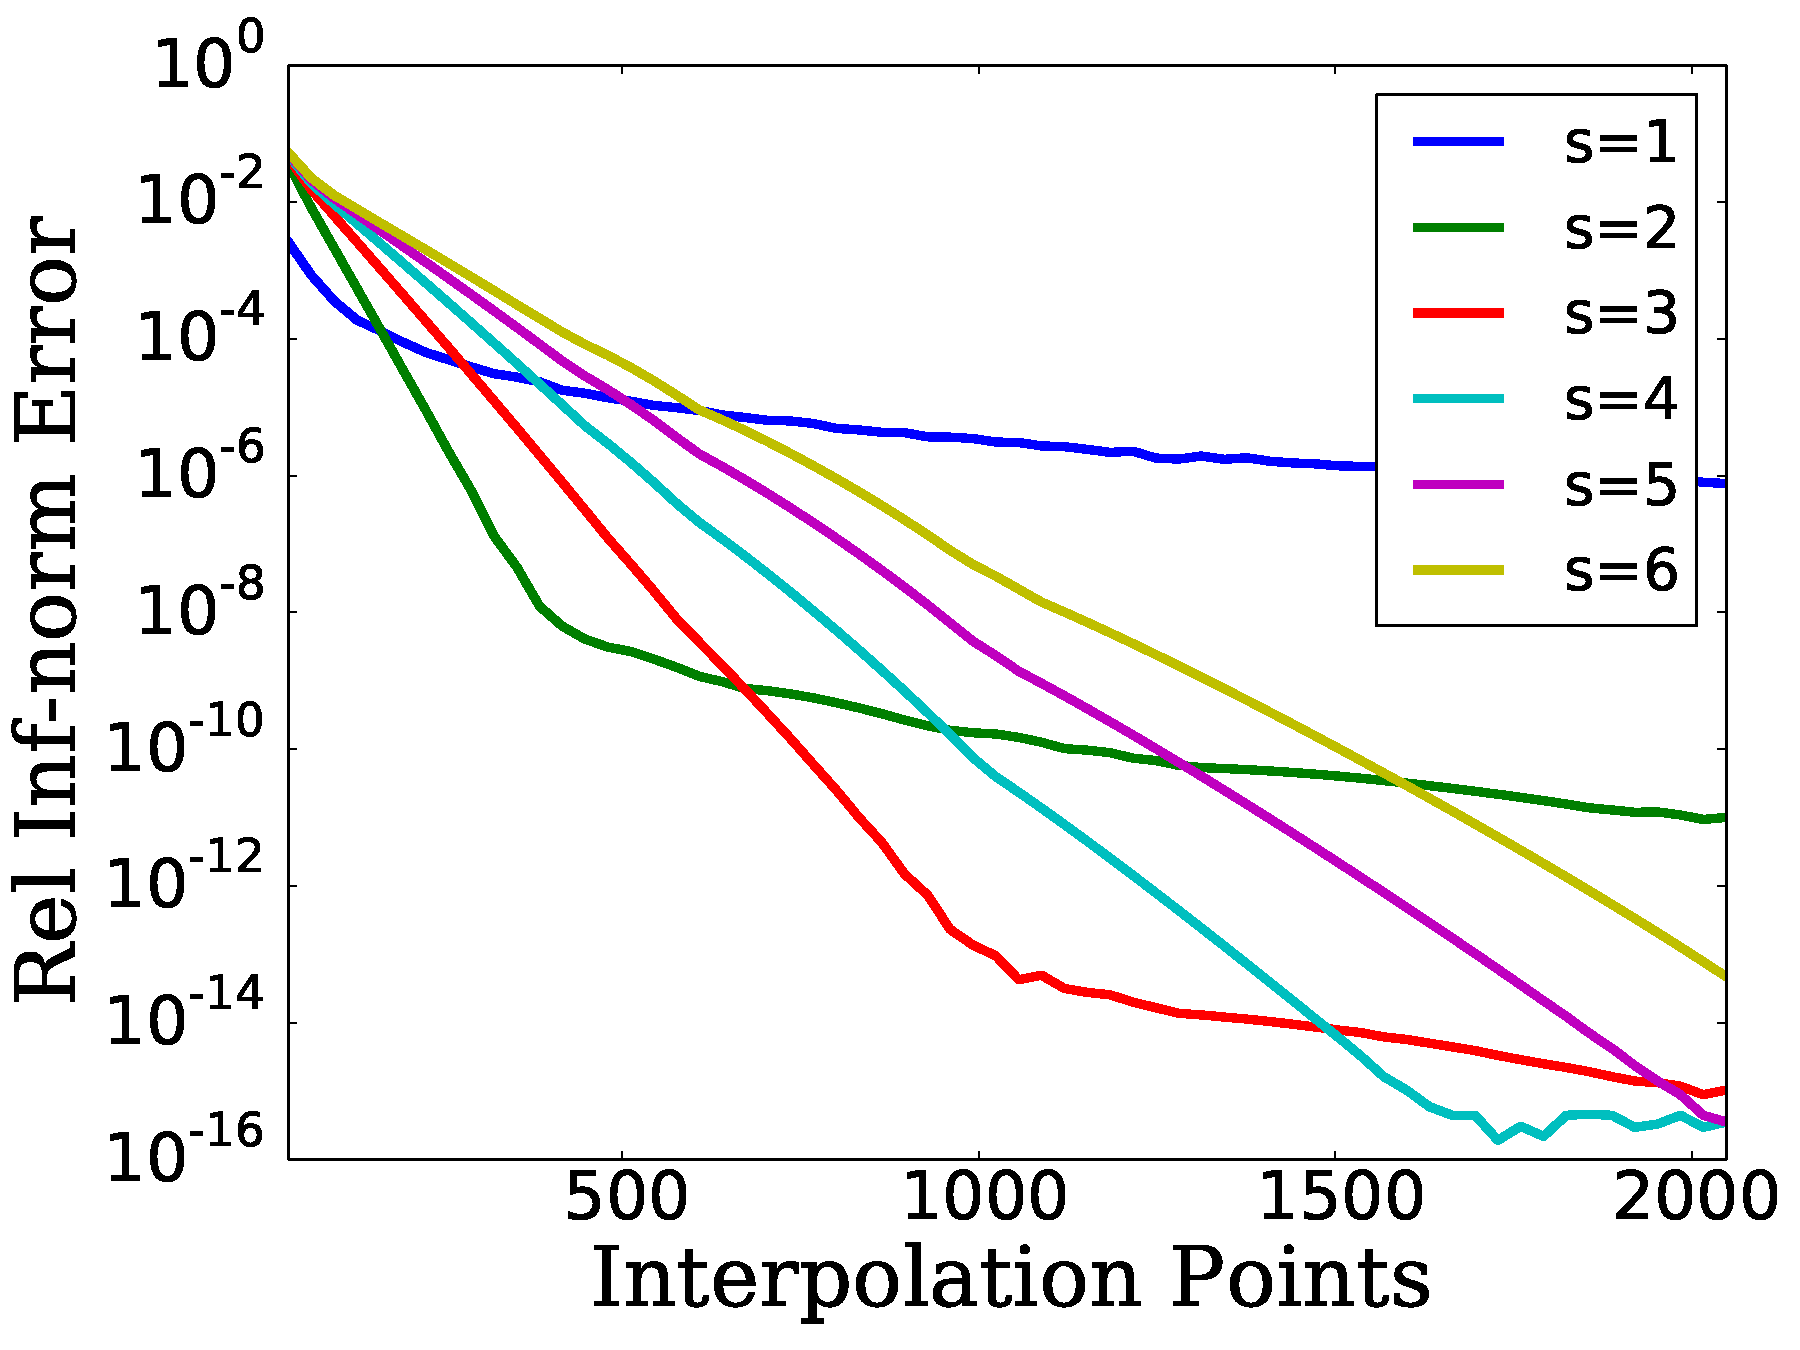
\includegraphics[width=\textwidth]{plots/msn_interp_fast_8n_rough_heaviside_2.pdf}
    \caption{Degree $8n$}
    \end{subfigure}
\caption[Example Plots of MSN Interpolation of Various Degrees]{
We show results for different interpolation degree.
For large $s$ values, there is no apparent advantage for using
a higher interpolation degree.
}
\label{fig:msn_comp_degree}
\end{figure}







\subsection{Birkhoff Interpolation Comparison}

We now look the Birkhoff interpolation problem when we have
a discontinuous derivative.
The results for interpolating $G(\cdot,0.5)$ can be found in 
Fig.~\ref{fig:rough_birkhoff_comparison_sharp_func};
we compare MSN interpolation results against applying standard
filters to the coefficients obtained from the solution
in Eq.~\eqref{eq:smooth_birkhoff_system}.
As we can see, MSN interpolation performs significantly better than
any of the filters; in fact, the MSN plot appears the same as
the corresponding plot in Fig.~\ref{fig:rough_comparison_sharp_func}
except for $s=1$.
Results for Birkhoff interpolation of $G_{2}(\cdot,0.5)$
can be found in Fig.~\ref{fig:rough_birkhoff_comparison_sharp_func_2}.
The results are nowhere near as good, and neither of the methods
(MSN or Chebyshev filters) perform well in this case.
Better results may be possible but likely require more
interpolation nodes.
In this case, even though the interpolation could be solved well
with MSN, in this case the Birkhoff interpolation problem 
for general functions cannot.

% Print results for comparing MSN with Heaviside jump function

\begin{figure}[p]
    \centering
    \begin{subfigure}{0.45\textwidth}
    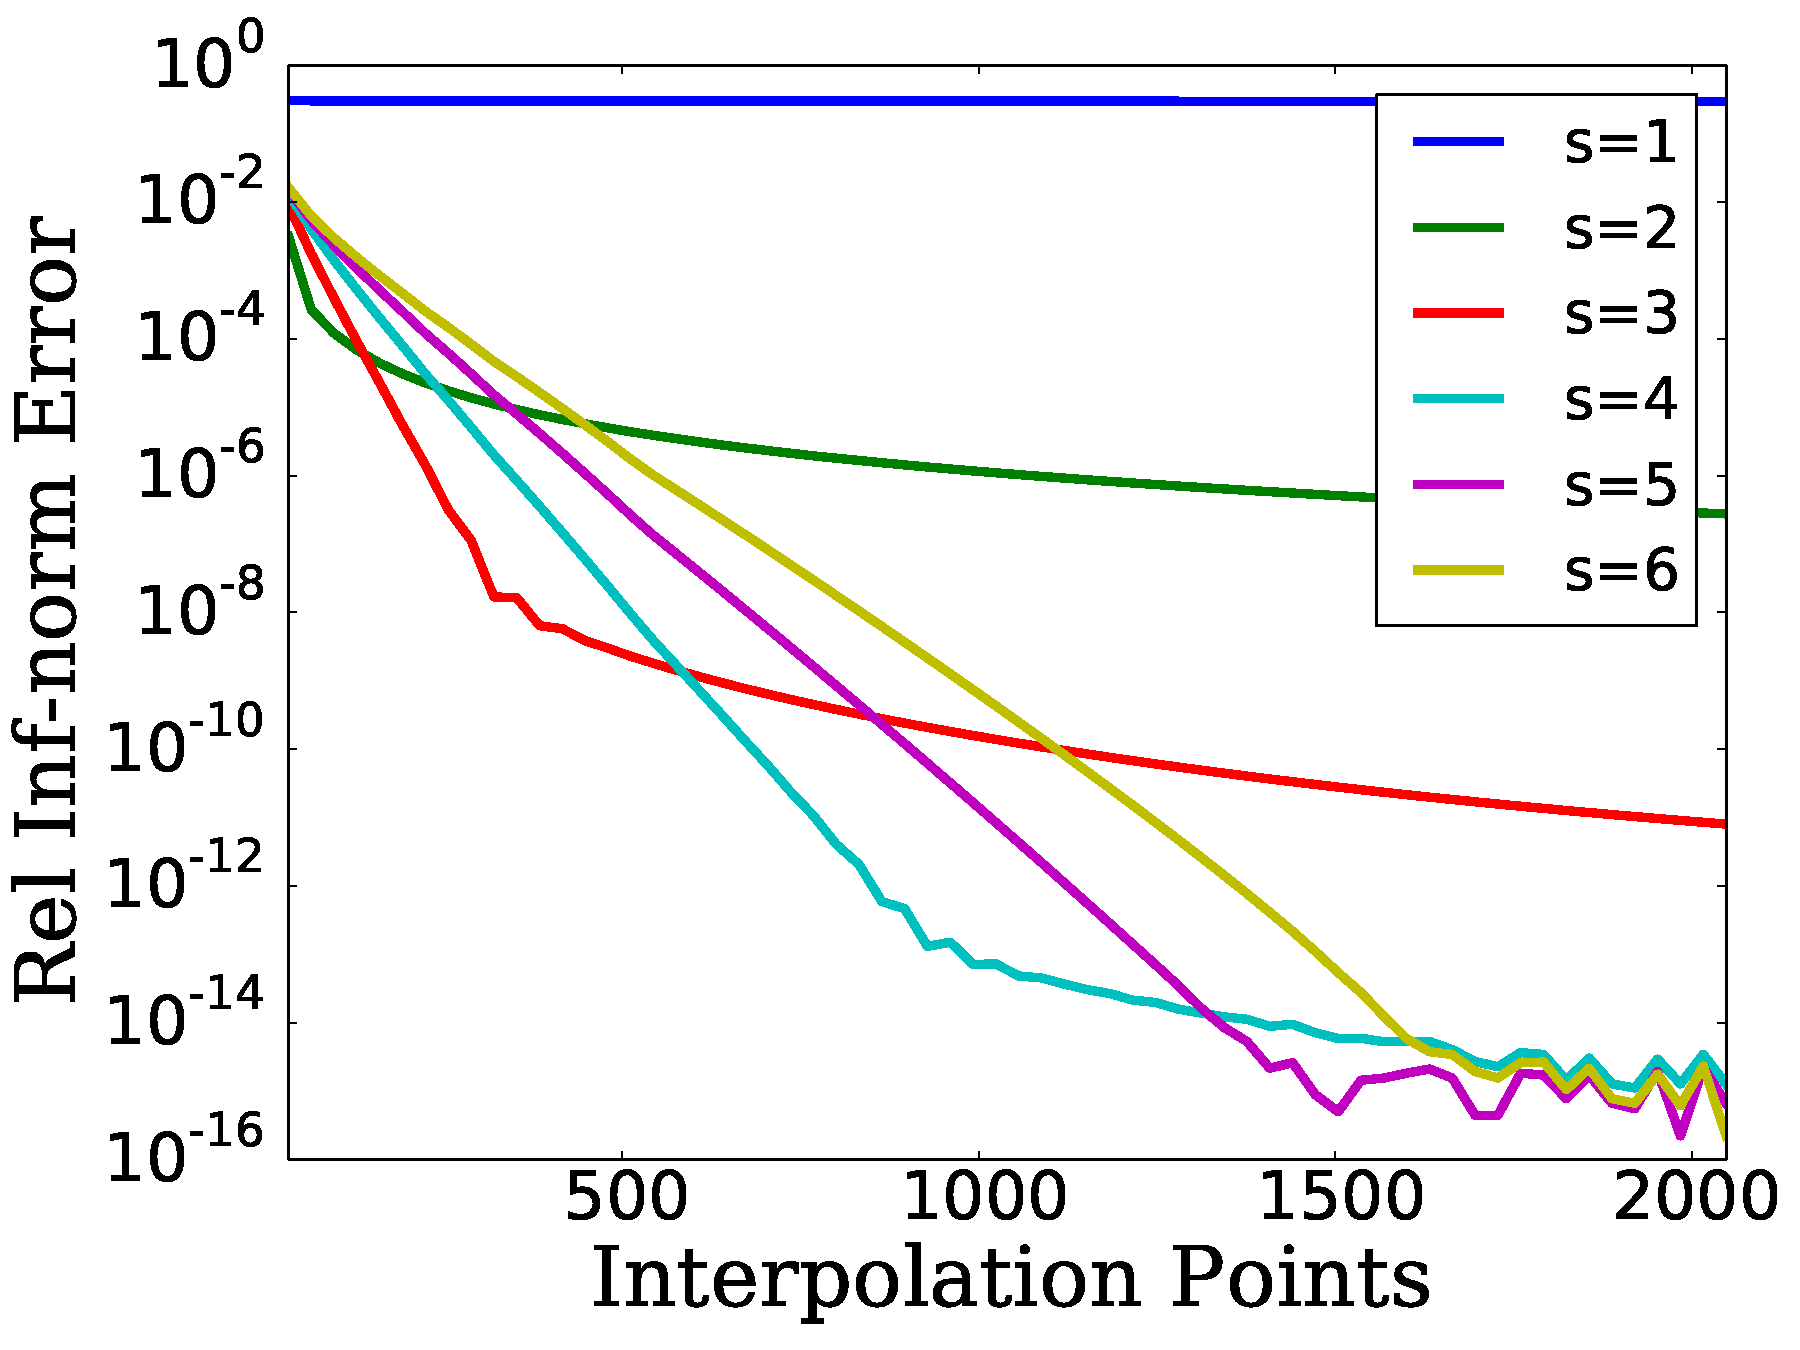
\includegraphics[width=\textwidth]{plots/msn_birkhoff_rough_sharp_funcs.pdf}
    \caption{MSN Interpolation}
    \end{subfigure}

    \begin{subfigure}{0.45\textwidth}
    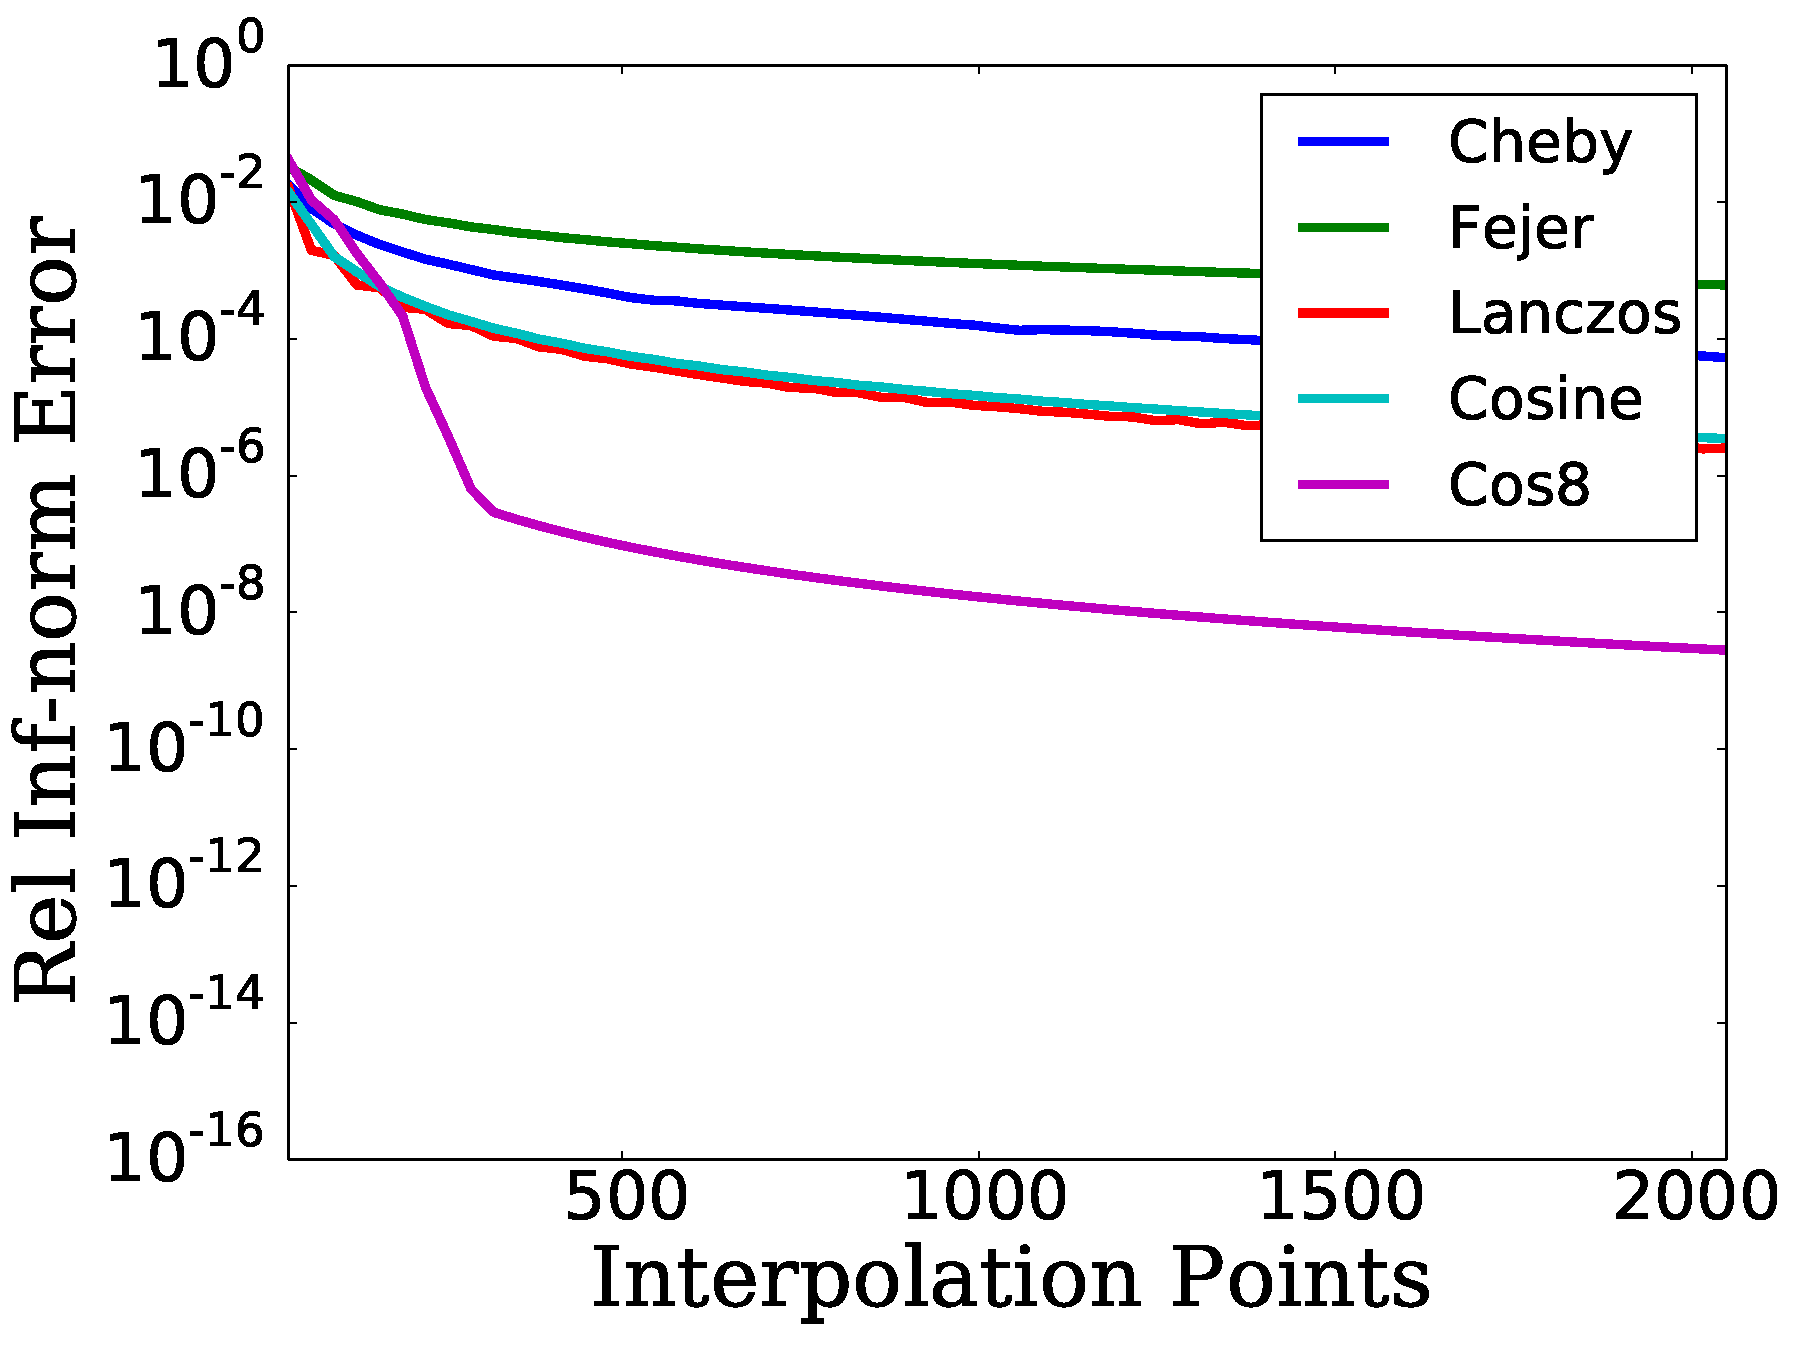
\includegraphics[width=\textwidth]{plots/cheby_birkhoff_filter_rough_sharp_func.pdf}
    \caption{Filters, Plot 1}
    \end{subfigure}
    \begin{subfigure}{0.45\textwidth}
    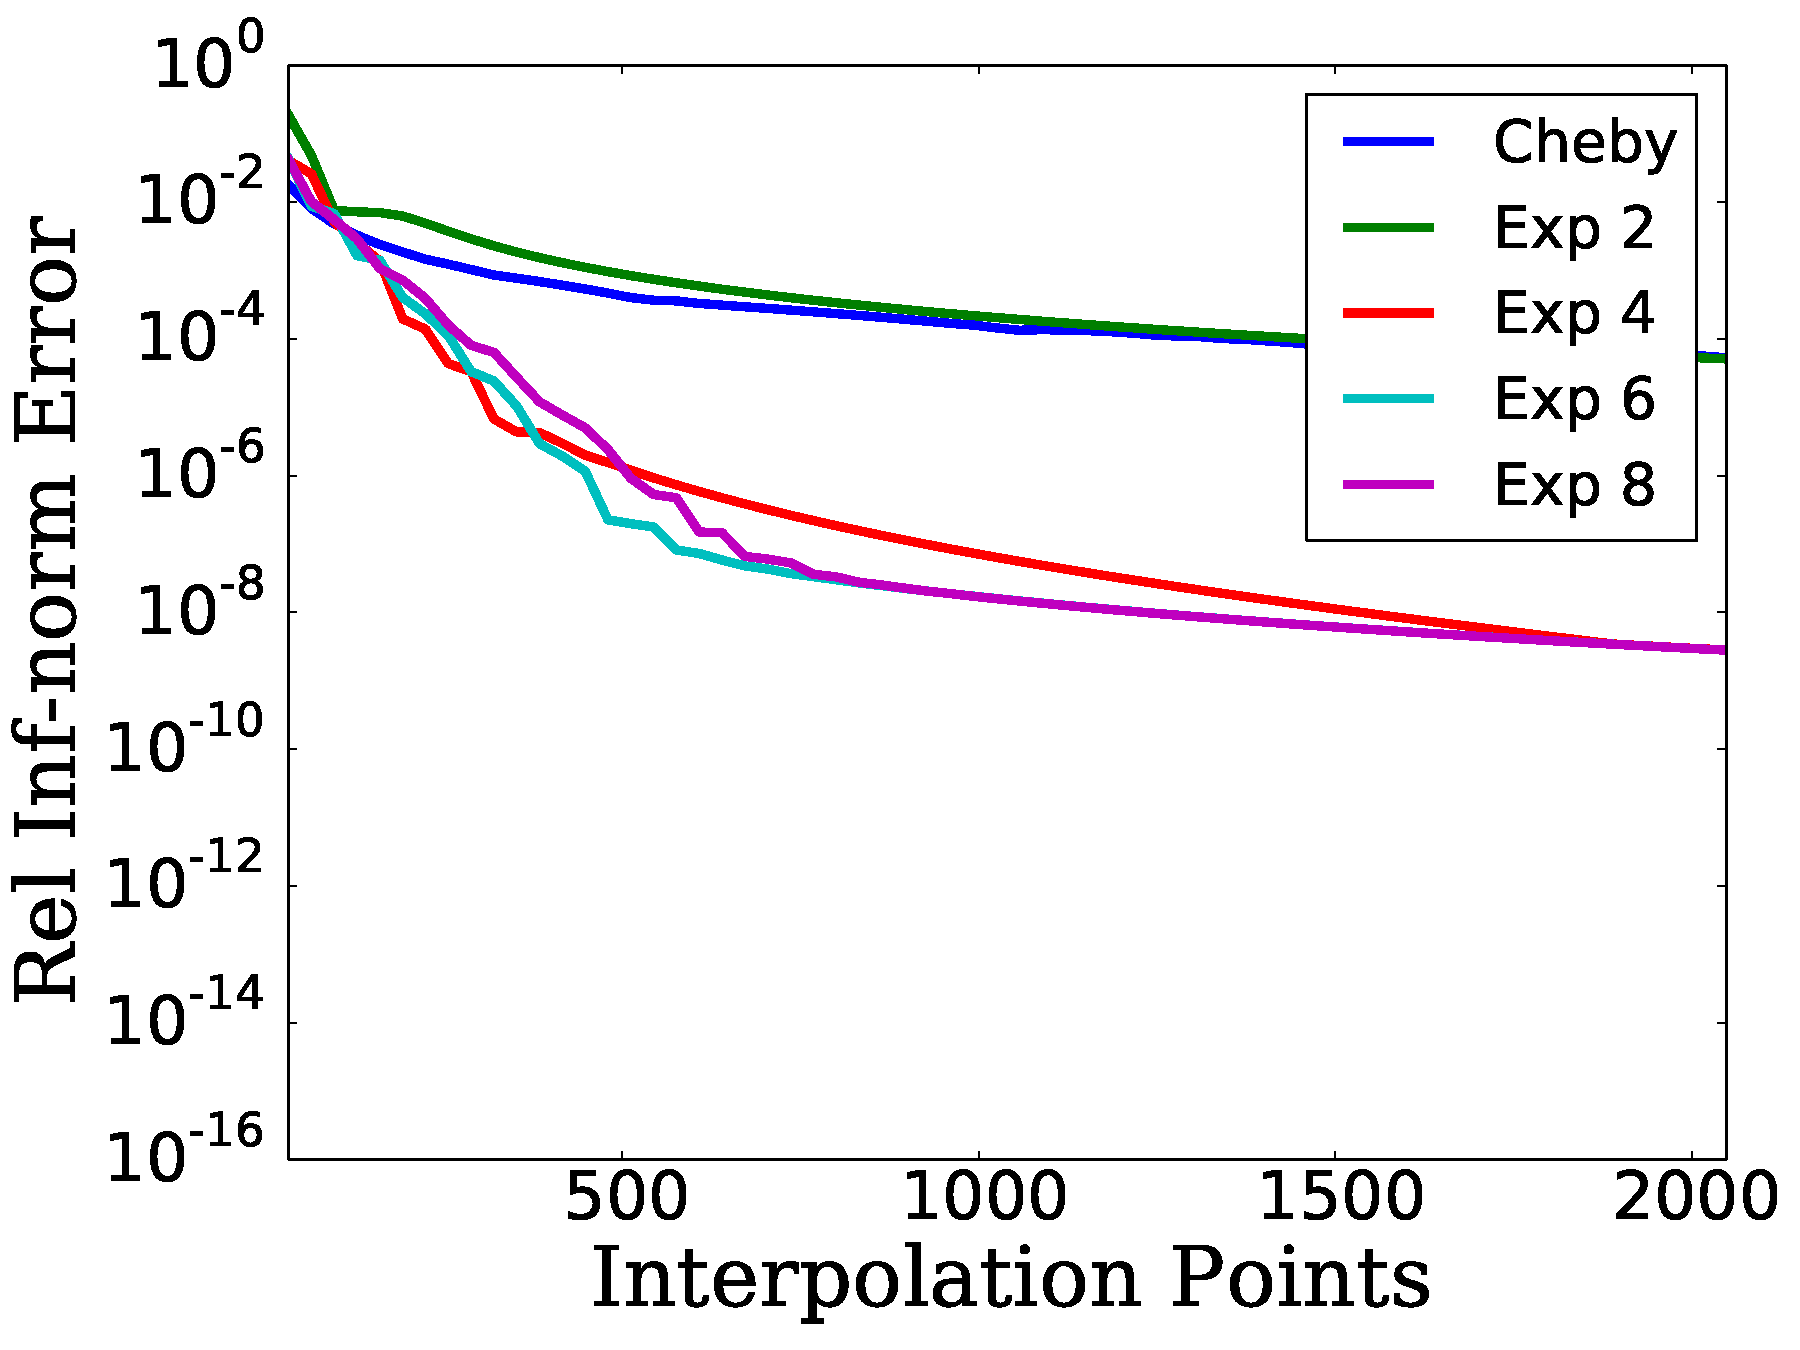
\includegraphics[width=\textwidth]{plots/cheby_birkhoff_filter_2_rough_sharp_func.pdf}
    \caption{Filters, Plot 2}
    \end{subfigure}
\caption[Rough Birkhoff Interpolation Comparison: Sharp Function]{
MSN interpolation and Chebyshev filtering results of the Sharp Function
$G(\cdot,0.5)$ for various $s$ values and filters.
We include standard Chebyshev birkhoff interpolant in both filter
examples for reference.
}
\label{fig:rough_birkhoff_comparison_sharp_func}
\end{figure}




% Print results for comparing MSN with Heaviside jump function

\begin{figure}[p]
    \centering
    \begin{subfigure}{0.45\textwidth}
    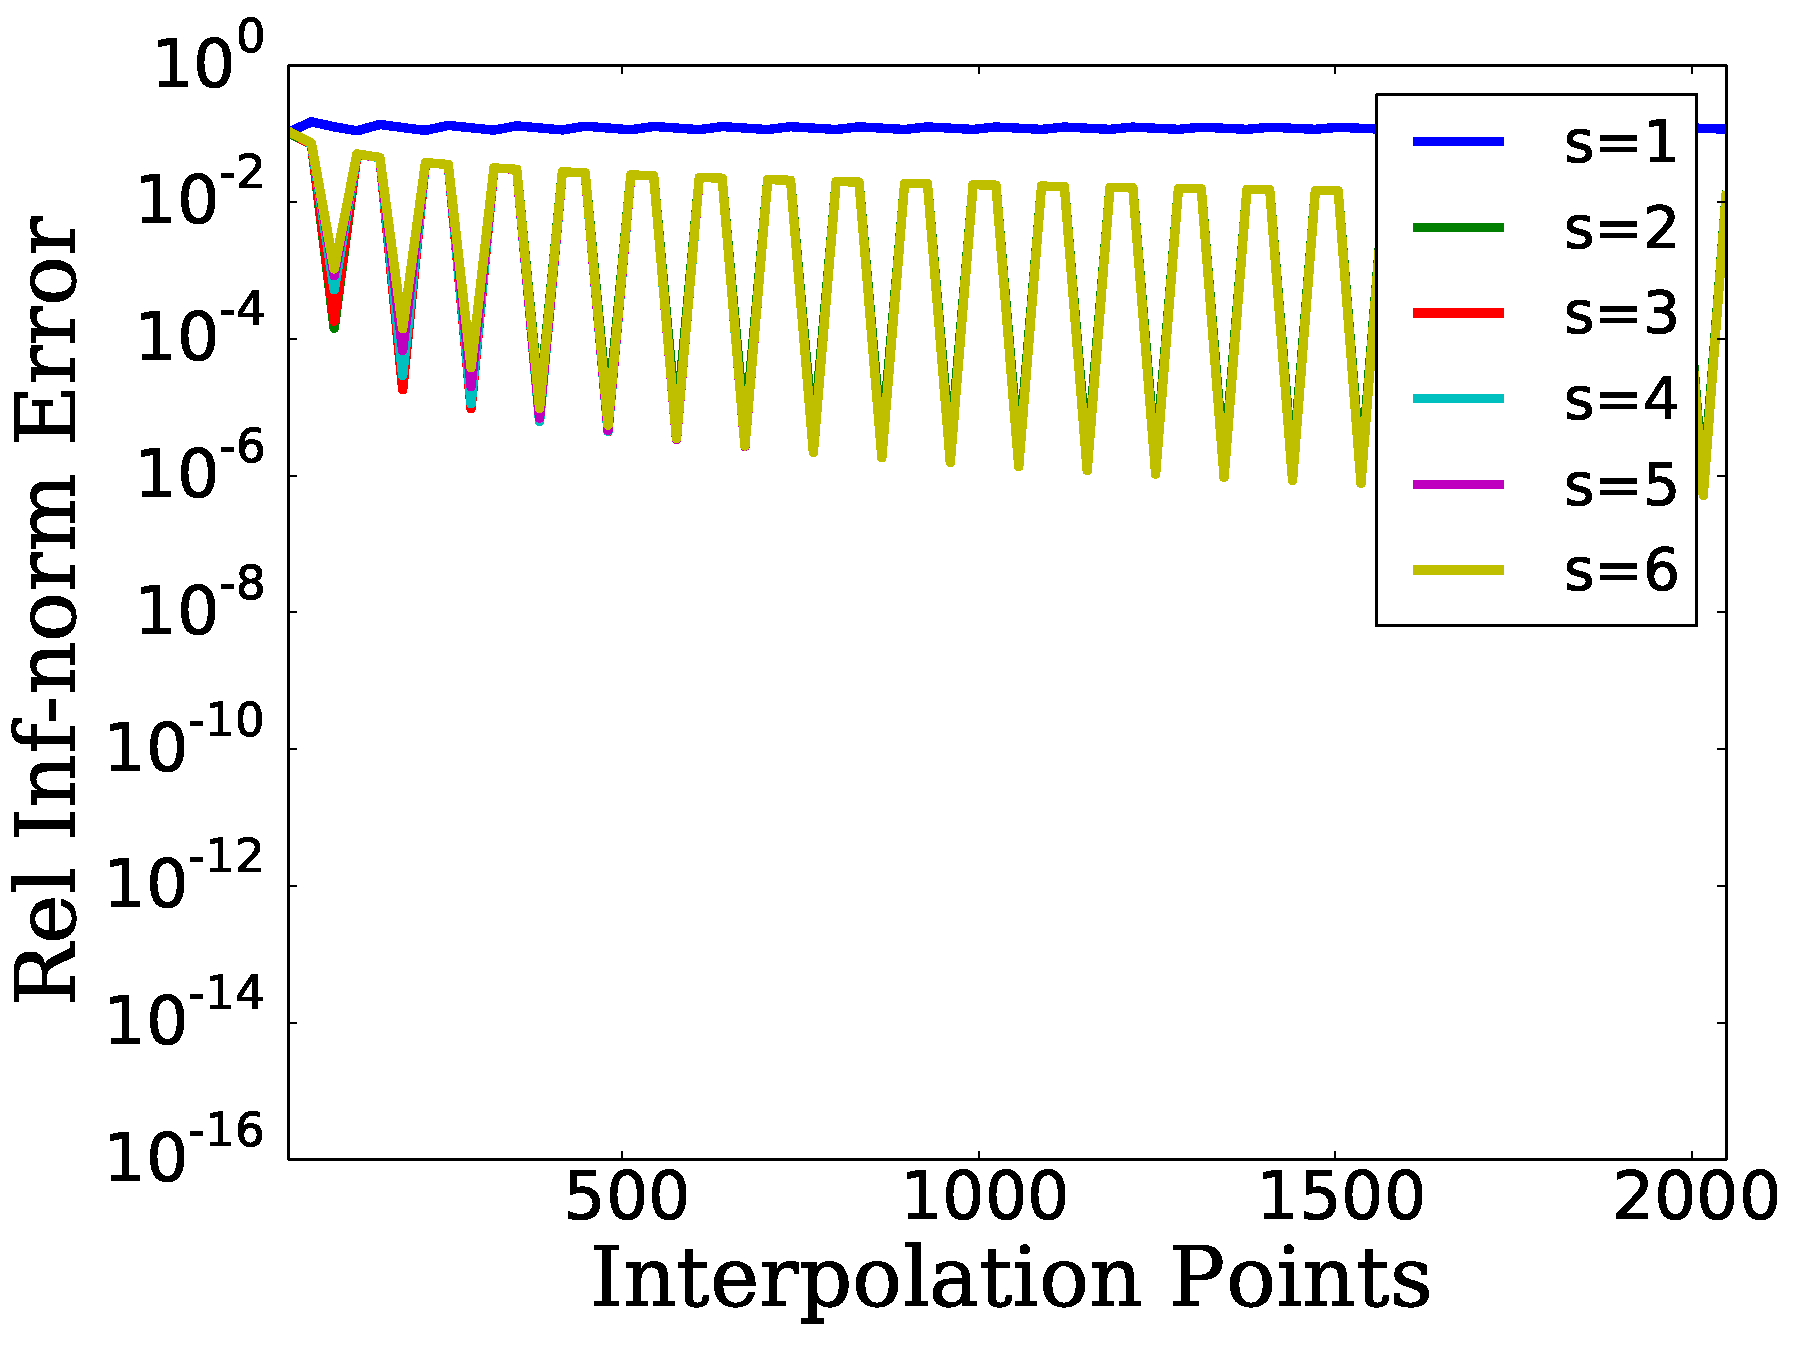
\includegraphics[width=\textwidth]{plots/msn_birkhoff_rough_sharp_funcs_2.pdf}
    \caption{MSN Interpolation}
    \end{subfigure}

    \begin{subfigure}{0.45\textwidth}
    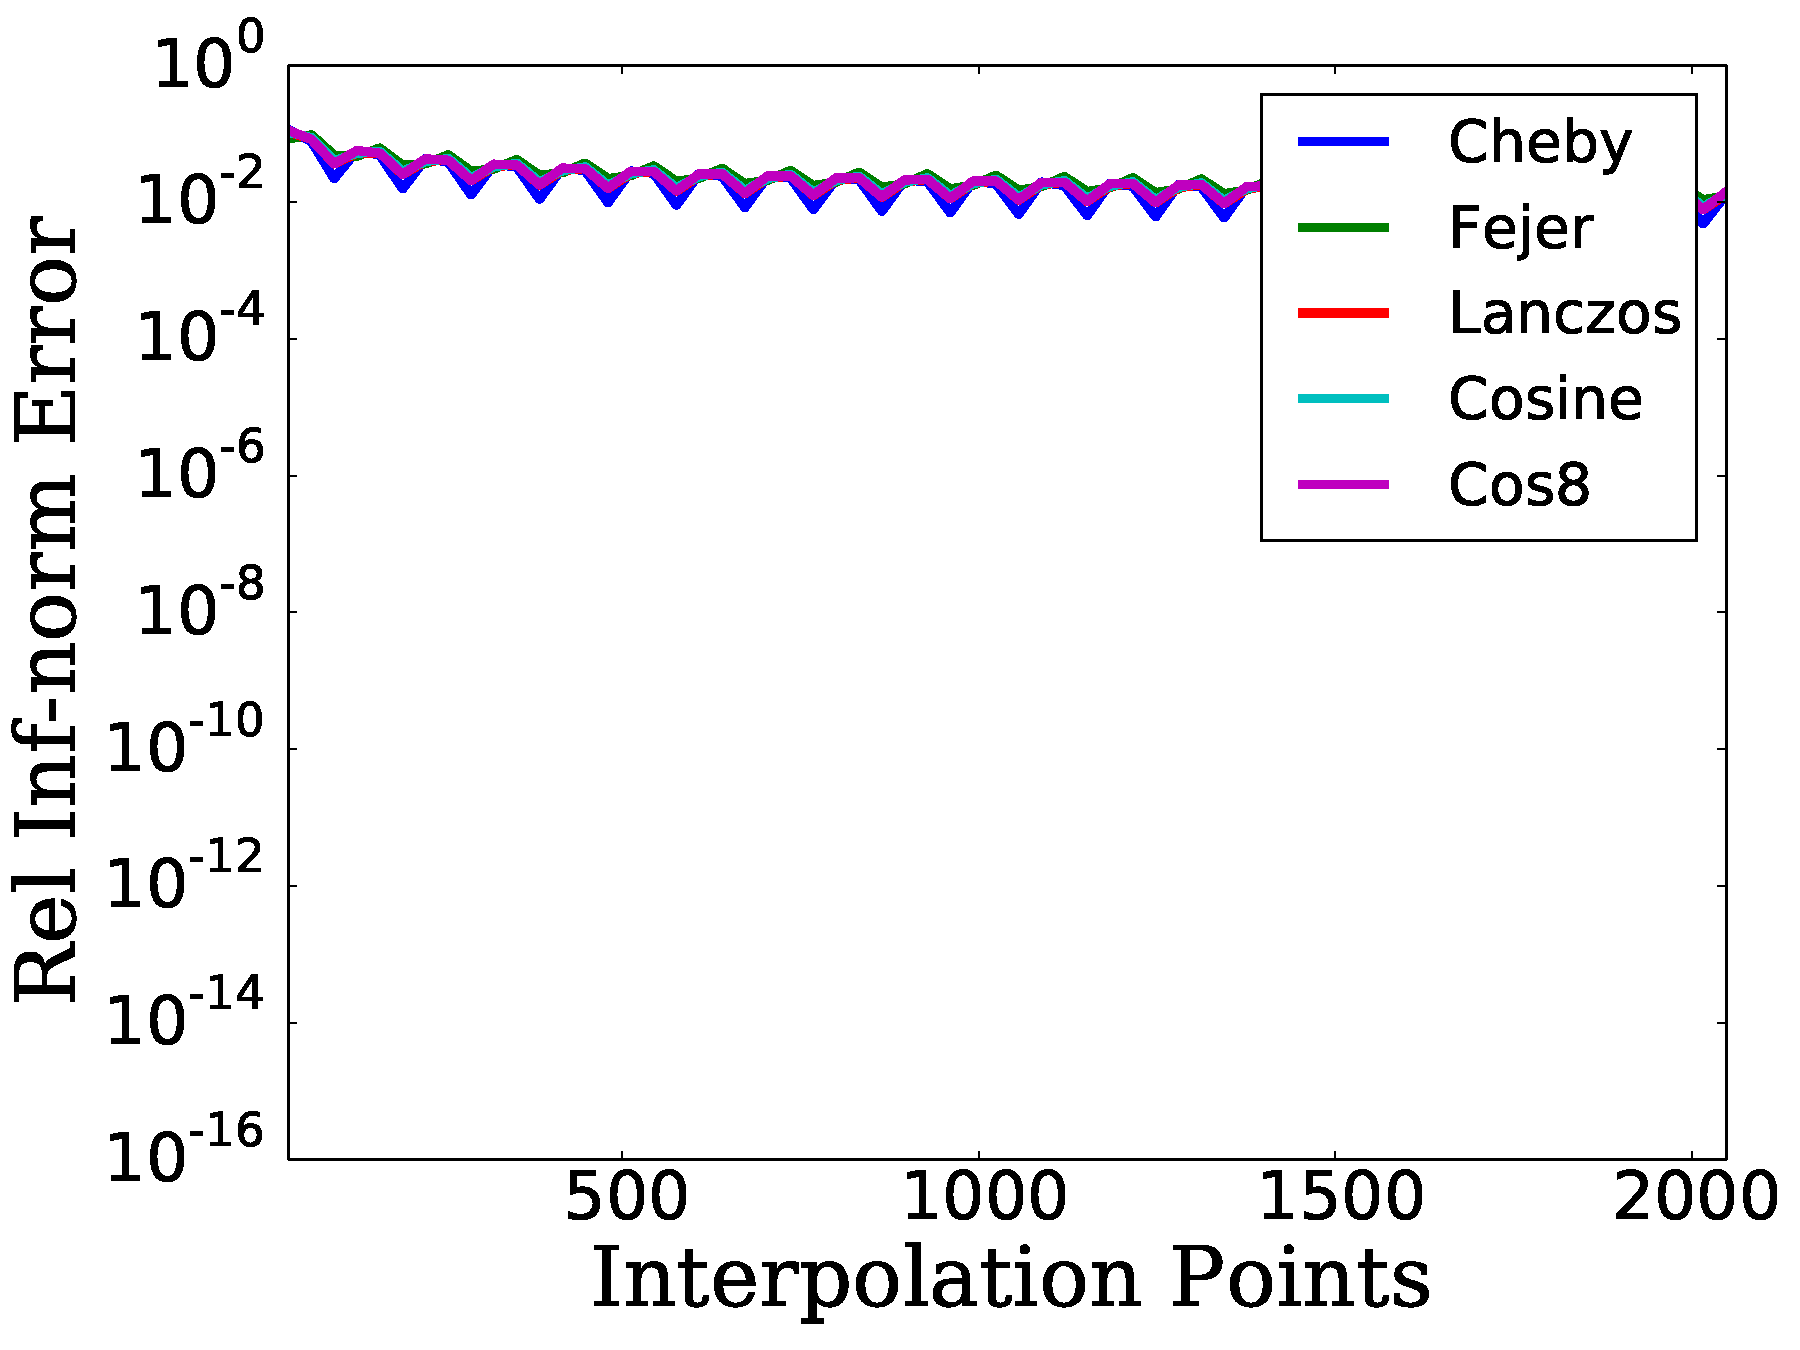
\includegraphics[width=\textwidth]{plots/cheby_birkhoff_filter_rough_sharp_func_2.pdf}
    \caption{Filters, Plot 1}
    \end{subfigure}
    \begin{subfigure}{0.45\textwidth}
    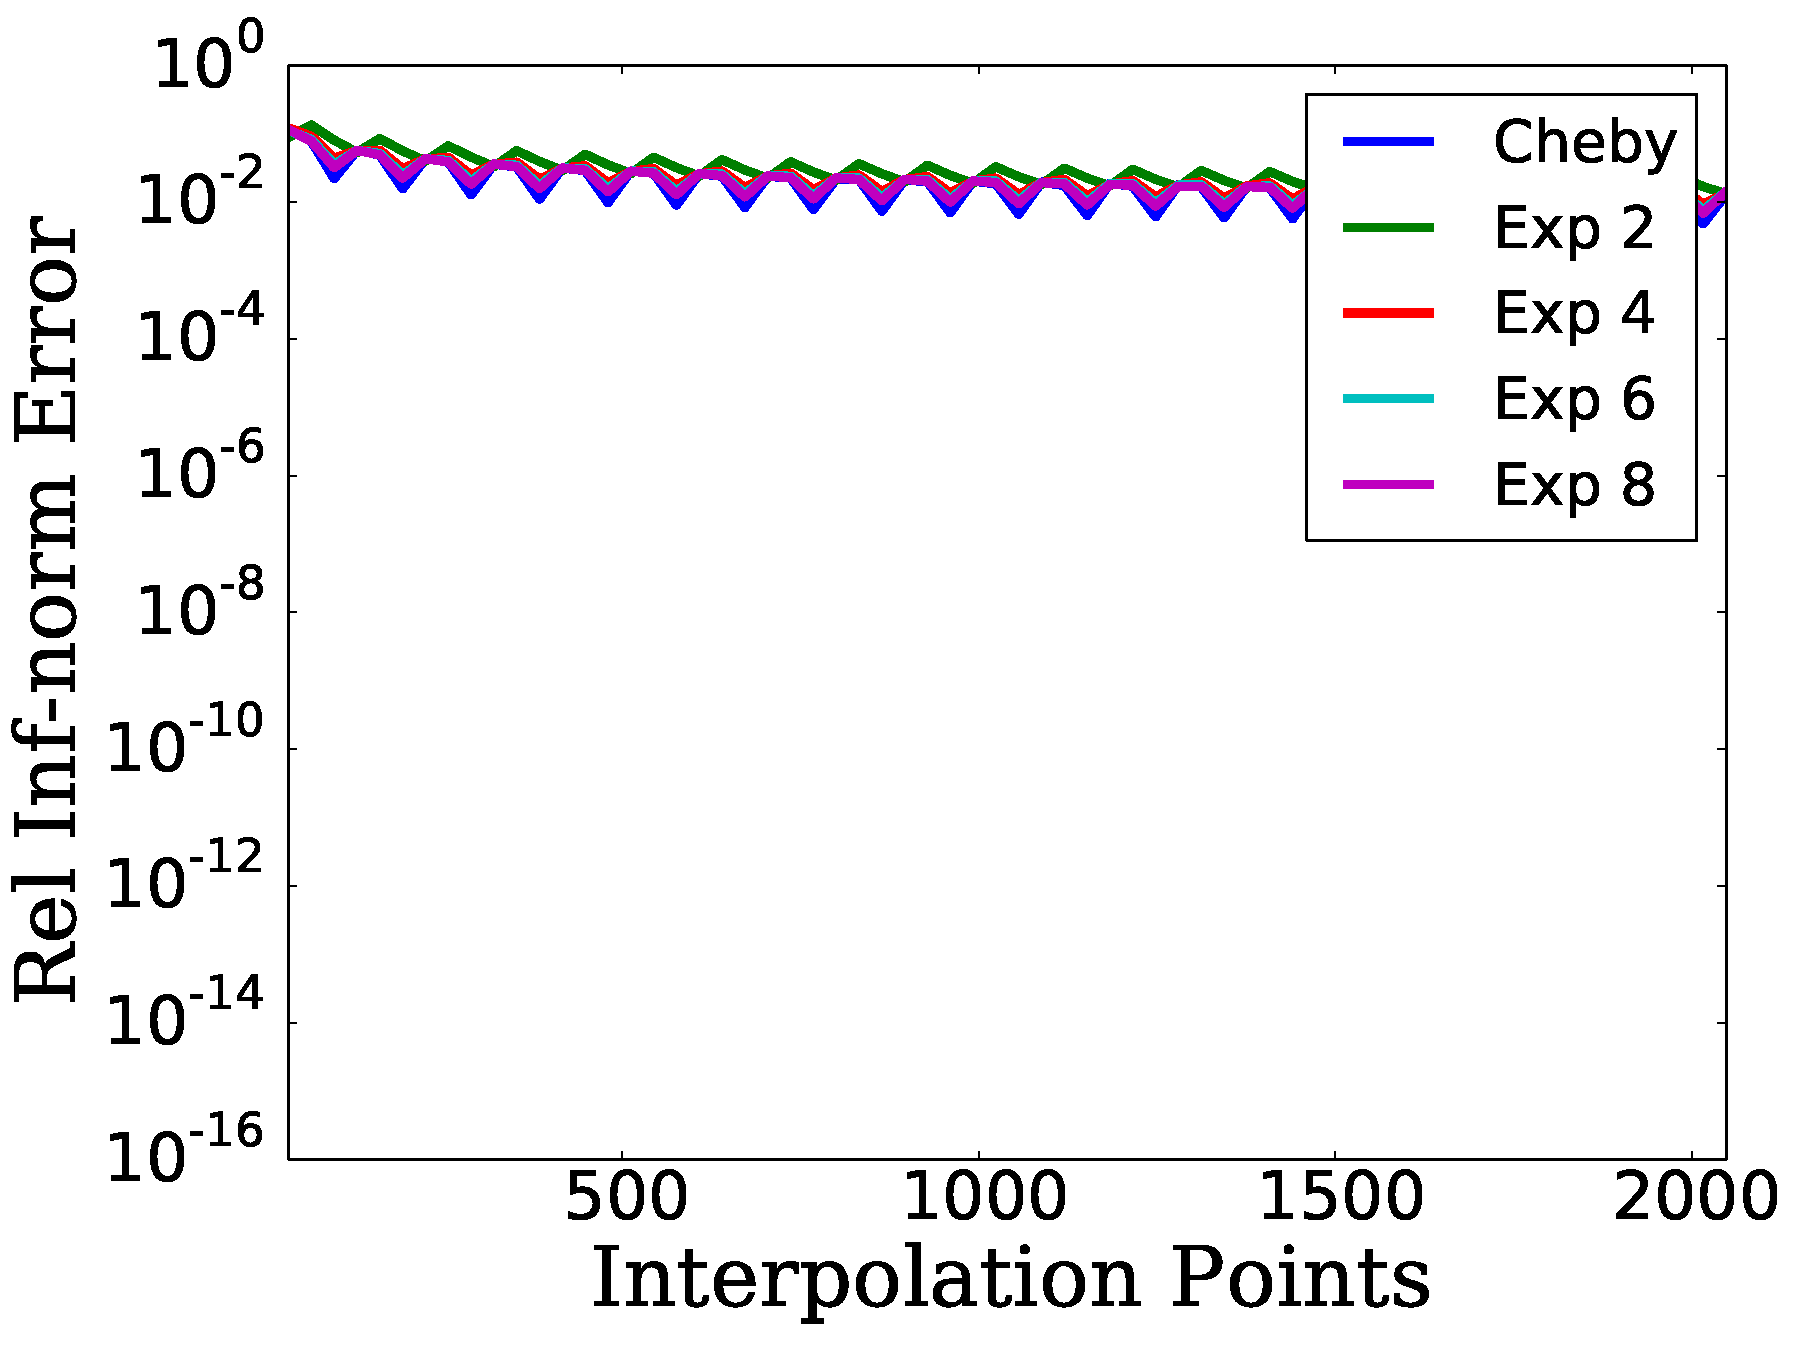
\includegraphics[width=\textwidth]{plots/cheby_birkhoff_filter_2_rough_sharp_func_2.pdf}
    \caption{Filters, Plot 2}
    \end{subfigure}
\caption[Rough Birkhoff Interpolation Comparison: Sharp Function 2]{
MSN interpolation and Chebyshev filtering results of the Sharp Function
$G_{2}(\cdot,0.5)$ for various $s$ values and filters.
We include standard Chebyshev birkhoff interpolant in both filter
examples for reference.
}
\label{fig:rough_birkhoff_comparison_sharp_func_2}
\end{figure}




